\chapter{Construction types} \label{ch:constructions}
\section{Introduction}

The last two chapters have presented a way to arrange the EI sample according to formal (Chapter \ref{ch:gram}) and semantic properties (Chapter \ref{ch:sem}). In the present chapter, I would like to combine the findings from both chapters into a typology of \textsc{multi-verb construction} types attestable throughout the EI languages. From the discussion in Chapter \ref{ch:gram} we have seen that dealing with the formal make-up of the constructions alone would hardly give rise to any meaningful analysis that can explain the semantic diversity in formally homogeneous constructions. This is clearly visible in the results from van Staden and Reesink's survey in at least three ways: First, the constructional schemas, such as independent serialisation, cover almost all of the semantic types across the different languages (cf. \citealt[34]{vanstaden2008serial}). Motion, direction, instrument, comitative, manner, and aspect can all be encoded as independent serialisation constructions. That is, both (or all) verbs are inflected for the language-specific \textsc{infl}-categories. Second, almost all semantic types are attested in more than one constructional pattern. For instance, direction is found to be encoded by all four construction types in different languages. And third and most confusingly, there are some languages which do not show strict rules as to the construction type used \citep[24f.]{vanstaden2008serial}. One case is Taba where a coreferential actor on the second verb can, but need not, be cross-referenced, effecting the optional use of either an independent  or a dependent serialisation pattern. In example (\ref{Tabap300}) below, the first sentence could equally be construed without verbal inflection on the second verb, while the second sentence would also be acceptable with inflected \textit{mul}. Bowden points out that the choice of the two constructions may be linked to different speech registers (slow and more careful in the first case, and casual and faster in the second) but there is no apparent difference in semantics or prosody \citep[300]{bowden2001taba}.

\ea \label{Tabap300}
\langinfo{Taba}{Austronesian, SHWNG}{\citealt[300]{bowden2001taba}}\\
\ea
\glll nhan nait tesu \\
n=han n=ait te-su \\
\textsc{3}\textsc{sg}=go \textsc{3}\textsc{sg}=ascend \textsc{neg}-\textsc{pot} \\
\glft `(S)he hasn't yet gone up.' \\ 
\ex
\glll ncopang mul hu \\ 
n=sopang mul hu \\
\textsc{3}\textsc{sg}=descend return \textsc{cont} \\
\glft `(S)he's still coming back down.'\\ 
\z
\z

Putting these findings together, we have to state that identical form (i.e., using the same formal feature values for a set of constructions) does not entail identical semantics, and vice versa. Rather, what we see is a set of complex relations between a small number of formal construction types based on parameters like argument interaction, headedness, and contiguity on the one hand, and a rather large number of `semantic' types that may be encoded by MVCs on the other. But does that mean that we simply cannot trace regular patterns or tendencies across this wealth of combinations? I think the answer is no. The patterns are there, they just don't come out so clearly if we don't distinguish between different kinds of semantic interaction between the verbs. To give an example, the boundary between \textsc{motion-to-action} (motion in van Staden and Reesink's terms) and \textsc{motion complex} (called direction in van Staden and Reesink) cannot be clearly drawn by just looking at the formal patterns of headedness alone. Both semantic types can occur in independent as well as in dependent serialisation. However, if we apply semantic criteria other than these, there are apparent boundaries, I claim, that divide a two-stage motion-to-action construal from a componential motion complex. 

In the previous chapter, I argued for three basic techniques of MVC formation, that is, \textsc{merging}, \textsc{modification}, and \textsc{staging proper}. A set of further MVC\\textscs do not seem to materialise on the clausal but rather on the discourse level. I have termed discourse-based MVC formation (free) juxtaposition. In what follows, I will shift the viewpoint from the formal and semantic types in the sense of van Staden and Reesink to these four techniques of semantic interaction between the verbs. In my view, it is the semantics of verbal interaction that gives rise to differences in coding properties, rather than the other way round. 

The techniques of MVC formation, I want to argue, give rise to four overall multi-verb construction types: merging is the underlying mechanism in \textsc{component-relating construction}s (CREL), modification gives rise to \textsc{modifying construction}s (MOD), staging proper leads to \textsc{stage-relating construction}s (SREL), and finally, juxtaposition yields \textsc{free juxtaposition construction}s (FJUX). As we run through the different instances of these types, it will become clear that there are both prototypical cases to be found in the EI sample as well as peripheral, sometimes even quite dubious, exemplars. My claim is not that these types are invariable across the EI languages or that they necessarily come with rigid boundaries. Rather, the idea is that the fundamental techniques of MVC formation may each lead to a family of MVC cases that is on the output level restricted by constraints in verbal interaction and by how linguistic communities conventionalise the different potential templates arising from them. 

This chapter proceeds as follows. I will first introduce these construction types with regard to their general properties. Postulating constructional types requires some kind of justification. Ideally, this includes criteria that help to distinguish between them. §\ref{sec:criteria_mvcs} will outline some potential tendencies that seem to be associated with some, but not with all types. In §\ref{sec:dist_types} I will have a look at their geographical distribution. The chapter then goes on to provide a typology of multi-verb constructions found in  the EI dataset. Each construction will be given with its formal properties and its distribution across the area, complemented with examples from different languages and subareas. 

\subsection{MVC types} \label{sec:mvc-types}

I will start by introducing the construction types that are associated with the four techniques from the previous chapter. This review will then lead to a comparison of these types. Component-relating constructions subsume those constructions that undergo merging of (parts of) their LS. In Chapter \ref{ch:sem}, I  discussed ways in which verbs may be decomposed into smaller chunks of meaning (the sublexical predicates), and how those might interact in a MVC. In component-relating constructions (\textsc{crel}), all verbs belong to the same lexical field, and thus share part of their LS. So, for instance, two motion verbs make up what I call a motion complex. The order of the verbs is fixed, and so is the specific bit of information that is contributed by each verb in the merging process. I assume that \textsc{crel} constructions provide a means of construing a tight event description in the sense that a separation of the first component from the second component is not possible on temporal grounds. For example, in a construction like (\ref{Waima'a119}) below, we would not want to say that there is an initial \textsc{stage} of the moving theme falling after which there is another stage of the same referent now (by acting deliberately) descending. 

\ea \label{Waima'a119}
\langinfo{Waima'a}{Austronesian, CMP}{pear\_Santina 119}\\
\glll inke ne ne lo'i rou leku \\
inike ne ne lo'i rou leku \\
which \textsc{foc} \textsc{3}\textsc{sg} fall descend \textsc{med} \\
\glft `And then he has fallen down there.' \\ 
\z

Quite to the contrary, one of the defining features of \textsc{crel} constructions is that each referent is only allocated one semantic role. In examples like (\ref{Waima'a119}) above the semantic role of the second verb gets overwritten by that of the first verb under the merging process. In this sense, it is not by deliberately descending that the referent moves downwards but by plain falling. The second verb then only contributes the path specification to the construction, as semantic role information is not preserved through the merging process.
 
If we now turn to stage-relating constructions (\textsc{srel}), we observe no such semantic role-spreading from V$_1$ to V$_2$. Rather, both verbs submit distinct event stages that in a temporal sense are related by pragmatic interpretation (such as a reading of immediateness of sequence) rather than by merging of their LS. Take the motion-to-action construction as an example. Although the construction by itself is prone to denote intention-action relationships (we seldom go somewhere without intending to do something there), sometimes the second verb does license an argument with a semantic role that seems different from the previous one. Most obvious examples include a stage of sleeping as for instance in the Hatam example below.

\ea \label{Hatam6465}
\langinfo{Hatan}{Papuan, Hatam-Mansim}{\citealt[108f.]{reesink1999grammar}}\\
\ea
\gll yoni y-ug bong ei ig-bei big, \\
they \textsc{3}\textsc{sg}-go sleep \textsc{loc} house-under not \\
\glft `They don't go (to) sleep in the house (at home),' \\ 
\ex
\gll noro y-ug bong ei bigbehei \\ 
but \textsc{3}\textsc{sg}-go sleep \textsc{loc} forest \\
\glft `but they go to sleep in the forest.' \\ 
\z
\z

The scene seems clear: There is a group of referents that moves deliberately to a certain place with the intention to lie down there and have a rest. While we know by inferring from the construction that their sleeping there was intended and not just, say, a chance result of sudden fatigue, we still wouldn't want to claim that the semantic role of the second stage is identical to that of the first. Intuitively, sleeping is an event that involves an undergoer referent rather than an actor. What we can see from examples like these, I conclude, is that there is no semantic merging between the LS of V$_1$ and V$_2$. The semantics of sleeping does not submit any specification to the motion stage denoted by V$_1$.

In modifying constructions (\textsc{mod}), on the other hand, we do find a semantic relationship between the verbs, but it is not of the component-relating kind. In \textsc{crel} constructions, we get verbs that denote fairly independent semantic concepts: they are active, actor-oriented and most of them readily occur in simplex predicate structures as they do in \textsc{crel}s. The defining verbs in \textsc{mod} constructions, on the other hand, tend to be stative rather than active, event rather than actor-oriented, and many of them are not frequently encountered in isolation (thus straddling the independent verb parameter often assumed to be part of SVCs). The group of \textsc{mod} constructions appears to be quite heterogeneous, at least at first blush. There is, however, a striking similarity in the semantic relationship between the verbs: the semantics are typically hierarchical in the sense that one verb lacks certain parts of a full-fledged \textsc{lexeme-level event}, and contributes an incomplete LS. Such verbs thus strongly resemble a modifier that morphosyntactically behaves like a verb. The semantics submitted by the modifier verb is not obligatory for the main verb in order to project a predication. They are optional, and only enrich the temporal or the participant frame of the construction. As discussed in the last chapter, a useful way to characterise the distinction between main verbs and modifier verbs in \textsc{mod} constructions is by making use of the so called Davidsonian notion of events (see e.g. \citealt{maienborn2011event}). In §\ref{sec:modification} I suggested that modifier verbs do have an event argument, yet it is spatiotemporally empty, and does not percolate upwards into the constructional scheme. It is rather the full-fledged main verb that contributes the exact spatiotemporal properties by submitting its event argument. The following example from Maybrat can be considered a typical example of a \textsc{mod} construction. 

\ea \label{}
\langinfo{Maybrat}{Papuan, isolate}{\citealt[207]{dol2007grammar}}\\
\gll t-fat ara m-kah pam \\
1\textsc{sg}-fell tree 3\textsc{u}-with axe \\
\glft `I fell a tree with an axe.'\\ 
\z

The last construction type to be discussed here is free juxtaposition (\textsc{fjux}). \textsc{fjux} is assumed to take place on the discourse level rather than on the level of the clause. The most clear-cut distinction is between \textsc{fjux} on the one hand, and \textsc{crel} and \textsc{mod} on the other as there is no direct interaction in \textsc{fjux} between the LS of the verbs involved. Rather, what is characteristic of \textsc{fjux} is that there is a more general relation of pragmatic association between the verbs in that either both predications are regarded as co-occurring on temporal grounds, or that the first predication temporally precedes the second one. Consider example (\ref{Mpurp99}) from Mpur:

\ea \label{Mpurp99}
\langinfo{Mpur}{Papuan, isolate}{\citealt[99]{ode2002sketch}}\\
\gll a-subwe be a-mesem ka n-wanem-i pan \\
\textsc{3}\textsc{sg}.\textsc{m}-follow but \textsc{3}\textsc{sg}.\textsc{m}-smell that \textsc{3}\textsc{sg}.\textsc{f}-stink-\textsc{cl} already \\
\glft `He followed her, but as he smelled, she already stank.' \\ 
\z

In example (\ref{Mpurp99}) we observe a combination of a clause coordination structure and an embedded \textsc{fjux} construction within the second constituent of the coordination. Both verbs in the \textsc{fjux} construction, \textit{mesem} `smell' and \textit{wanem} `stink', are delivered without formal signs of co- or subordination. However, what is typically observed in \textsc{fjux} constructions (and exemplified here in (\ref{Mpurp99})) is that i) the verbs do not necessarily share an argument (\textit{mesem} here seems to be intransitive and does not directly license the second referent which, however, is easily retrievable from the discourse space), ii) operators do not necessarily target both verbs (\textit{pan} appears to reinforce a reading of cotemporality here in that it marks the second predication as already being true at the time of his smelling), and (iii) most instances of \textsc{fjux} appear to be biclausal rather than monoclausal. From an event perspective, the biclausal appearance of many \textsc{fjux} suggests that both verbs appear to denote distinct CLEs that, by pragmatic inference, may be interpreted to occur within the same stretch of time. That is, I suppose that although it may appear as if the event arguments of both verbs were matched, this only takes place on the level of pragmatic interpretation.

\subsection{Criteria for distinction of MVC types}\label{sec:criteria_mvcs}

In this section, I will have a closer look at how these constructional families might be set off against each other in ways that seem applicable across different linguistic profiles. To this end, I will suggest a set of criteria. Most of these criteria may not apply categorically in each case, but they do at least indicate tendencies at which points the types may be expected to deviate from one another. When applied together, I suppose that the values cluster around the proposed types. Table \ref{table:criteriaconstruction} provides an overview of the proposed criteria.

\begin{table}
\begin{tabular}{lrrrr}
\lsptoprule
Criteria&CREL&SREL&MOD&FJUX\tabularnewline
\hline
\tabularnewline
\textit{Argument structure}& & & & \tabularnewline
Obligatory argument interaction&yes&yes&yes&no\tabularnewline
Event-to-argument reanalysis&(yes)&no&yes&no\tabularnewline\tabularnewline
\textit{Operator behaviour}& & & & \tabularnewline
Identical TAM/person index values&yes&yes&yes&no\tabularnewline
Partial temporal modification&no&yes&no&yes\tabularnewline
Partial negation&no&no?&yes&yes\tabularnewline\tabularnewline
\textit{Constituency}& & & & \tabularnewline
Obligatory constituent order&yes&yes&no&yes\tabularnewline
Asymmetrical headedness&yes&yes&yes&no\tabularnewline
MVC embedding (stacking)&no&yes&yes&yes\tabularnewline
Conjunction insertion&no&no&no&yes\tabularnewline\tabularnewline
\textit{Semantic properties}& & & & \tabularnewline
Sequential reading&no&yes&no&yes\tabularnewline
Temporal immediacy&no&yes&no&no\tabularnewline
Grammaticalisation of features in V$_1$&no&yes&yes&no\tabularnewline
Grammaticalisation of features in V$_2$&yes&no&yes&no\tabularnewline
\tabularnewline
\lspbottomrule
\end{tabular}
\caption[Criteria to distinguish MVC types]{Criteria to distinguish MVC types attested in the EI data set. \textsc{crel} - component-relating constructions, \textsc{srel} - stage-relating constructions, \textsc{mod} - modifying constructions, \textsc{fjux} - free juxtaposition constructions. Brackets indicate that contradicting values only occur with a small number of examples or in few languages.}
\label{table:criteriaconstruction}
\end{table}

Some of the criteria from Table \ref{table:criteriaconstruction} have already been discussed, or at least mentioned, in the previous chapters (such as argument interaction, operator values or headedness), and I will only make brief reference to them. Some other criteria, on the other hand, seem to have been evaluated rarely or not at all in the literature, and seem promising for future work on MVCs. Note that, as these criteria cluster around the MVC types, they are not independent in the sense that they could be expected to show just any value, but rather interdependent because they are linked to the underlying techniques of MVC formation. Take the parameter of partial temporal modification. Partial temporal modification in two-stage constructions like \textsc{srel}s must be licit as every stage is supposed to be projected from a spatiotemporally definable event argument. In the same way, the two-stage property also causes \textsc{srel}s to permit MVC embedding into one of their constructional slots. In fact, most of the criteria that I will briefly present in the remainder of this section seem to be interdependent, thus pointing to more general properties of the MVC types.

There are two criteria from \textsc{argument structure} that appear to cluster with MVC types in the EI dataset. Obligatory argument interaction subsumes both the argument sharing options discussed in §\ref{sec:argumentstructure} (same subject, switch-function, and participant accumulation) as well as event-to-argument reanalysis. All three monoclausal constructions types, \textsc{crel}, \textsc{srel} and \textsc{mod}, require their arguments to interact with one another. They may be shared, or the first LLE may be reanalysed as the subject of the second one. In contrast, the various biclausal MVCs placed in the category \textsc{fjux} in this book do not require such an interaction, as we have seen, for instance, in example (\ref{Mpur50}) at the end of Chapter \ref{ch:sem}. If we have a closer look at the distribution of argument interaction types across the three aforementioned types, we can conclude that at least staging proper is not compatible with event-to-argument reanalysis, basically because staging involves a sequence of PLEs across which at least one of the referents needs to be kept constant. This assumption is indeed borne out by the data, as we will see in §\ref{sec:stage-relating} on stage-relating constructions.

\textsc{Operator behaviour} can provide another three criteria that help distinguish between MVC types. Intuitively, \textsc{fjux} constructions are free to denote any operator value in each of their parts. This is to be expected if these parts really constitute full-fledged clauses each with its own inflectional head. The monoclausal construction types, on the other hand, should not be able to denote different operator values. This seems to be so at least with regard to the verbal categories used throughout the EI area, that is, TAM categories and person indexing morphology. A related yet different type of operator is temporal modification via adverbials. From a semantic perspective, temporal adverbials need to target a spatiotemporally definable event. In other words, we need to expect the target of such a modifier to provide an event argument in the Davidsonian sense. As only \textsc{srel} and \textsc{fjux} constructions provide more than \emph{one} independent event argument, it is only in these construction types that we find partial temporal modification. Recall example (\ref{WMH_Julio_goat099}) from Waima'a at the beginning of Chapter \ref{ch:sem} where the aspectual particle \textit{lo} seemed to align only with the motion phase but not with the subsequent action phase of the \textsc{srel} construction. Partial temporal modification is not acceptable with construction types that only consist of one spatiotemporal event stage, as in \textsc{crel} and \textsc{mod} constructions. Note that this constraint is in line with Bohnemeyer \& colleagues' macro-event property (MEP) concept (see \citealt{bohnemeyer2007principles, bohnemeyer2011}).

Another difference between the four types is found with partial negation. It might be hypothesized that partial negation is only applicable to those event construals that are made up of different spatiotemporal stages which then are either said to be true or not true. The \textsc{crel} and the \textsc{fjux} family of constructions appear to conform to this hypothesis. While \textsc{fjux} constructions may freely take a negator with limited scope over one of its constituents, \textsc{crel} constructions never occur with partial negator scope in the EI sample. This hypothesis, however, turns out to make wrong predictions as to the other two types. As \textsc{mod} constructions are one-stage constructions, one would not assume that partial negation is licit here. Occasionally, we do find cases with operators placed in positions that seem to suggest a partial scope. In Bunaq, for instance, \citet[451]{schapper2009bunaq} argues for partial negation in a case of ambient serialisation where a \textsc{know} verb is followed by a negator, and an intensifier verb in V$_2$.

\ea \label{}
\langinfo{Bunaq}{Papuan, TAP}{\citealt[451]{schapper2009bunaq}}\\
\gll eto hilaq bai tara niq masak o! \\
2\textsc{sg} \textsc{surprise} thing know \textsc{neg} big \textsc{emph} \\
\glft `Gosh, you don’t know a thing greatly!' (i.e. `Gosh, you know nothing!')\\ 
\z

Reverse cases are also found, in which it is the modifier verb that appears to be the only element negated. Negation in \textsc{mod} constructions may even occur as a lexicalised part of the modifier verb's meaning (for instance, in negative pseudo-modals that translate as `cannot'). The difference between one-stage negation and two-stage negation is that only in the latter case does the negator target a full event argument. The case with \textsc{srel} constructions is especially unclear: on the one hand, different stages should enable the negation of one stage without also negating the other. We have already seen in the Alamblak example (\ref{alamblak1}) from §\ref{sec:gramprop} that at least in some languages basically every verbal constituent can receive partial negation in multi-stage constructions. However, other authors seem to assume that partial negation may turn \textsc{srel}s into biclausal structures (see for instance \citealt[184]{donohue1999} on Tukang Besi). 

\textsc{Constituency} provides some further critera that are worth exploring. I have already mentioned that a strong constraint on MVC formation is the iconicity of order (see also \citealt{vanstaden2008serial}). What happens first in the event line is placed first in the linguistic construal. This holds true for all cases of staging, that is, for stage-relating constructions (staging proper) and free juxtaposition (if sequential eventualities are involved). Single-stage constructions, that is component-relating constructions or modifying constructions, do not show this iconicity of order as there is no temporal substructure associated with their parts. What they do show, however, is a split into constructions with obligatory constituent order, and others with free order. 

I assume from what the EI sample shows that \textsc{crel}s in all languages from all subareas are construed with a common template, allocating the final slot to path or ground-denoting verbs in motion \textsc{crel}s, and to \textsc{say} verbs in speech act \textsc{crel}s. This template most probably arises from general characteristics in the diachronic formation of this MVC type. \textsc{mod} constructions, on the other hand, do not develop fixed templates across the EI area. For instance, aspectual \textsc{mod}s with \textsc{finish} verbs may come in either order: \textsc{finish} -- matrix verb, or matrix verb -- \textsc{finish}. I assume that as the \textsc{mod} family mainly comprises constructions that are on their way to being grammaticalised, this variation in constructional templates reflects different grammaticalisation pathways up to the point where modifying constituents may be moved around freely, even within single languages. This is, for instance, observable with case-marking MVCs developing towards verbal predicates with ordinary case-marked NPs. Thus, the criterion of free constituent order has two possible interpretations: first, the order of modifier and modified may vary between languages (given that we can identify a single construction), and second, the order of modifier and modified may be subject to variation on the actual utterance level within single languages. Both are facets of the broader observation stated in chapter \ref{ch:sem} that modification in MVCs is an undirected process (as opposed to component-relating constructions where merging is from V$_{fin}$ to V$_1$).

Three further criteria apply to a subset of MVC families at the constituency level. Asymmetrical headedness is found in all those constructions in which the verbs do not receive the same inflectional marking, comprising patterns with the first or the final verb bearing inflection (``1" and ``2", respectively), as well as cases with shared affix sets (``S"). If \textsc{fjux} constructions are indeed formed on the discourse level and consist of syntactically independent constituents, one might expect that they would not allow asymmetrical headedness. The EI dataset supports this assumption, and I will show in §\ref{sec:fjux} that there are only a handful of \textsc{fjux} constructions that deviate from symmetrical head-marking. MVC embedding has already been introduced in §\ref{sec:stackedmvcs}, and we have seen further examples throughout the previous chapter in which one MVC hosts another MVC within one of its constructional slots. MVC embedding is not uncommon in the multi-stage types \textsc{srel} and \textsc{fjux}. Some \textsc{mod} types also allow embedded MVCs. Yet \textsc{stacked MVCs} do not seem to occur with \textsc{crel} constructions at the matrix level. \textsc{Crel}s may be embedded into, say, the motion slot of motion-to-action \textsc{srel}s, but no MVC may fill the slot of a component-relating construction. Finally, conjunctions may optionally be inserted into (some) \textsc{fjux} MVCs, but there are no instances of optional junctors in any of the other constructional families.

A final group of criteria is \textsc{semantic} in origin. A sequential reading of the verbal constituents is found in the two-stage families \textsc{srel} and \textsc{fjux}, but not in \textsc{crel} and \textsc{mod} constructions. Sequential action, however, does not automatically entail a reading of temporal immediacy. In my understanding, we only find such interpretations in \textsc{srel}s. So, for instance, in \textsc{cause-result} or resultative constructions, it has frequently been noted that the resultant action or state is interpreted as happening or holding true immediately after the causing action has come to its end. We have already seen in §\ref{sec:gramprop} that this reading of immediacy is no longer a necessary prerequisite when we change the Paamese cause-result construction from example (\ref{paamese1}) by adding an overt subject expression to the second predicate (cf. example (\ref{paamese2})). In either case, hitting the pig results in its death, yet only the SVC marks the death as following immediately from the causing action. 

The last two criteria are diachronic citeria that are difficult to pin down by comparing languages without historical records. However, a synchronic comparison of the constructions from the different constructional families across EI shows two opposing tendencies in component-relating and in stage-relating constructions. In both constructional families, there are slots that host verbs from specific classes, for instance, directed motion verbs or \textsc{say} verbs in V$_2$ of component-relating constructions, and motion verbs, posture verbs or verbs of handling in V$_1$ of stage-relating constructions. These verbs seem to be prone to becoming grammaticalised, developing grammatical functions and losing (part of) their lexical semantics. Such grammaticalisation clines can be observed in different EI languages to varying degrees. This is not to claim that every verb in such a position will become grammaticalised after a certain amount of time. Rather, given the chance that some grammaticalisation will occur over time, it seems a fair guess that the defining verbs in these constructional slots will be more likely to grammaticalise than verbs from the other slots.

As I cautioned earlier these criteria are not meant to be `hard' criteria in the sense that they are expected to apply to each case. If anything, the EI sample shows that there are exceptions in every single constructional category, i.e. cases that are particularily hard to intepret, and so produce fuzzy boundaries between different MVCs. I take this fuzziness to be at least partially related to a prototype structure of the MVC families. As a construction is in use, progressive language users will quite naturally push it beyond its conventionalised frontiers, giving rise to unusual verb combinations, new ways of operator placement, and so on. Given this variation, the set of criteria is probably only helpful when the criteria are applied together (at best supplemented with further criteria yet to be identified). Only then do they indicate (some of) the dividing lines between the four constructional types \textsc{crel}, \textsc{srel}, \textsc{mod}, and \textsc{fjux}. 

I will now in the following section turn to the distribution of these MVC families across language families, subareas, and single languages.

\subsection{Distribution of MVC types}\label{sec:dist_types}

All four MVC types are found all throughout Eastern Indonesia. Table \ref{table:MVCtypes_overview} gives the overall numbers for the sample. From a total of 2146 instances found, the family of modifiying constructions scores highest with an overall 802 cases. This is consistently so, with regard to linguistic affiliation as with regard to areal subgroups. The only exception to the latter is Western Papua where both \textsc{crel} and \textsc{srel} constructions are more prevalent in the dataset. \textsc{fjux} constructions are overall a more peripheral phenomenon in the dataset, accounting for only 202 cases.

\begin{table}
\begin{tabular}{lrrrr}
  \lsptoprule
 & \textsc{crel} & \textsc{srel} & \textsc{mod} & \textsc{fjux} \tabularnewline 
  \hline
  Austronesian & 291 & 332 & 409 & 90 \tabularnewline
  Papuan & 246 & 273 &  393 &  112  \tabularnewline
   \hline
  Sulawesi & 39 & 75 & 133 & 21 \tabularnewline
  Nusa Tenggara & 225 & 196 & 355 & 83 \tabularnewline
  Maluku & 55 & 72 & 118 & 28 \tabularnewline 
  Papua & 218 & 262 & 196 & 70 \tabularnewline 
\lsptoprule
Total & 537 & 605 & 802 & 202 \tabularnewline
\lspbottomrule
\end{tabular}
\caption[Distribution of MVC types]{Distribution of MVC types across EI. \textsc{crel} = component-relating constructions, \textsc{srel} = stage-relating constructions, \textsc{mod} = modifying constructions, \textsc{fjux} = free juxtaposition constructions.}
\label{table:MVCtypes_overview}
\end{table}

What is remarkable about these numbers is that the proportion of instances from each construction type remains rather constant. As Figure \ref{fig:type-family} illustrates, both Papuan and Austronesian languages contribute about 36 to 38\% instances of \textsc{mod} constructions to the sample, followed by some 26 to 29\% \textsc{srel}s, 24 to 25\% \textsc{crel}s, and about 8 to 11\% \textsc{fjux} constructions. Given that the compilation of the sample involved different data sources, and avoided obvious biases by the authors by also sampling data from unrelated parts of the publications, this outcome seems notable. This distribution might suggests that linguistic affiliation is not a primary factor influencing the use or disuse of MVC types in EI, at least not from an overall perspective.

\begin{figure}
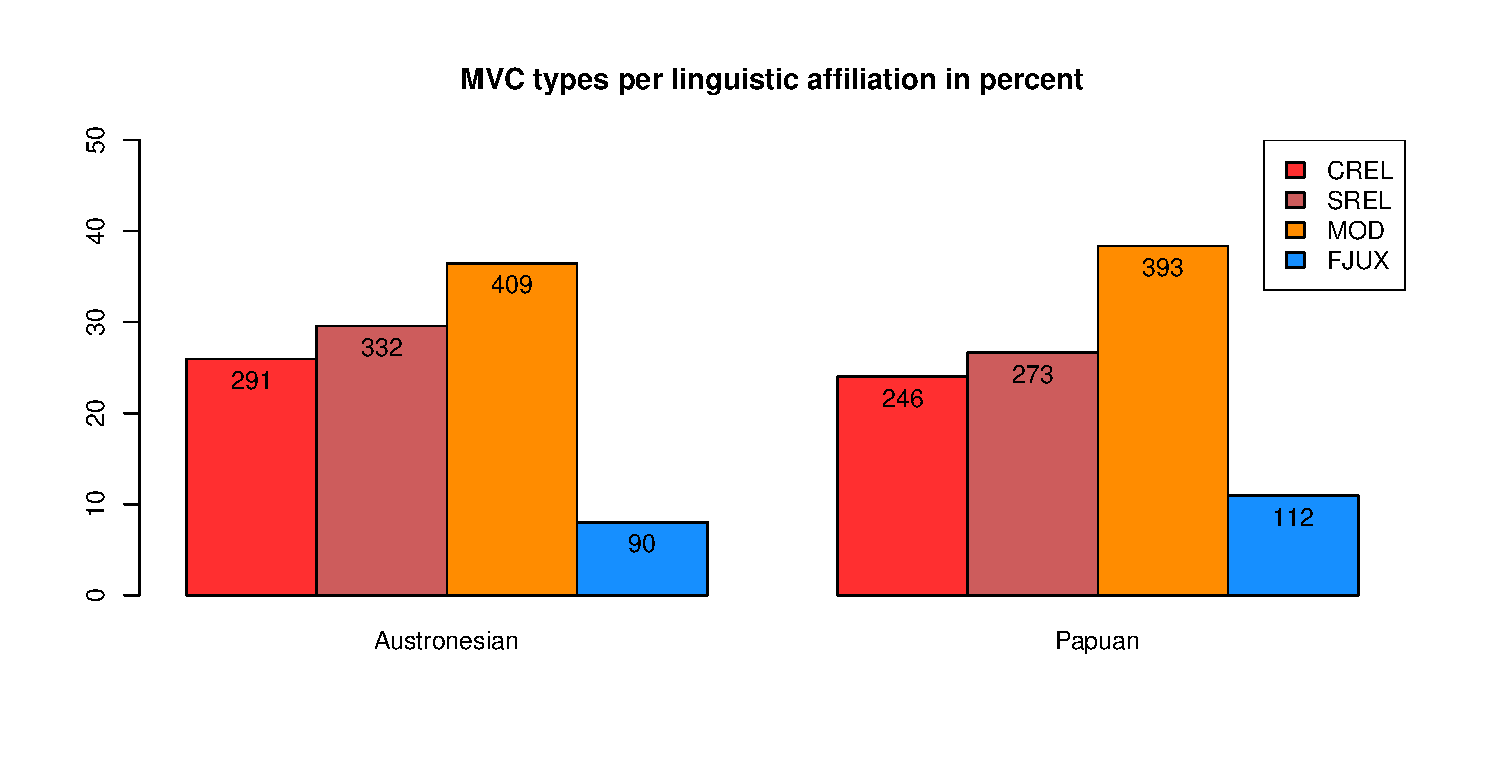
\includegraphics[width=\columnwidth]{figures/Type_Family.eps}
\caption[MVC types per linguistic affiliation in percent]{MVC types per linguistic affiliation in percent. \textsc{crel} = component-relating constructions, \textsc{srel} = stage-relating constructions, \textsc{mod} = modifying constructions, \textsc{fjux} = free juxtaposition constructions. Numbers on top of the bars refer to the number of observations.}\label{fig:type-family}
\end{figure}
\begin{figure}
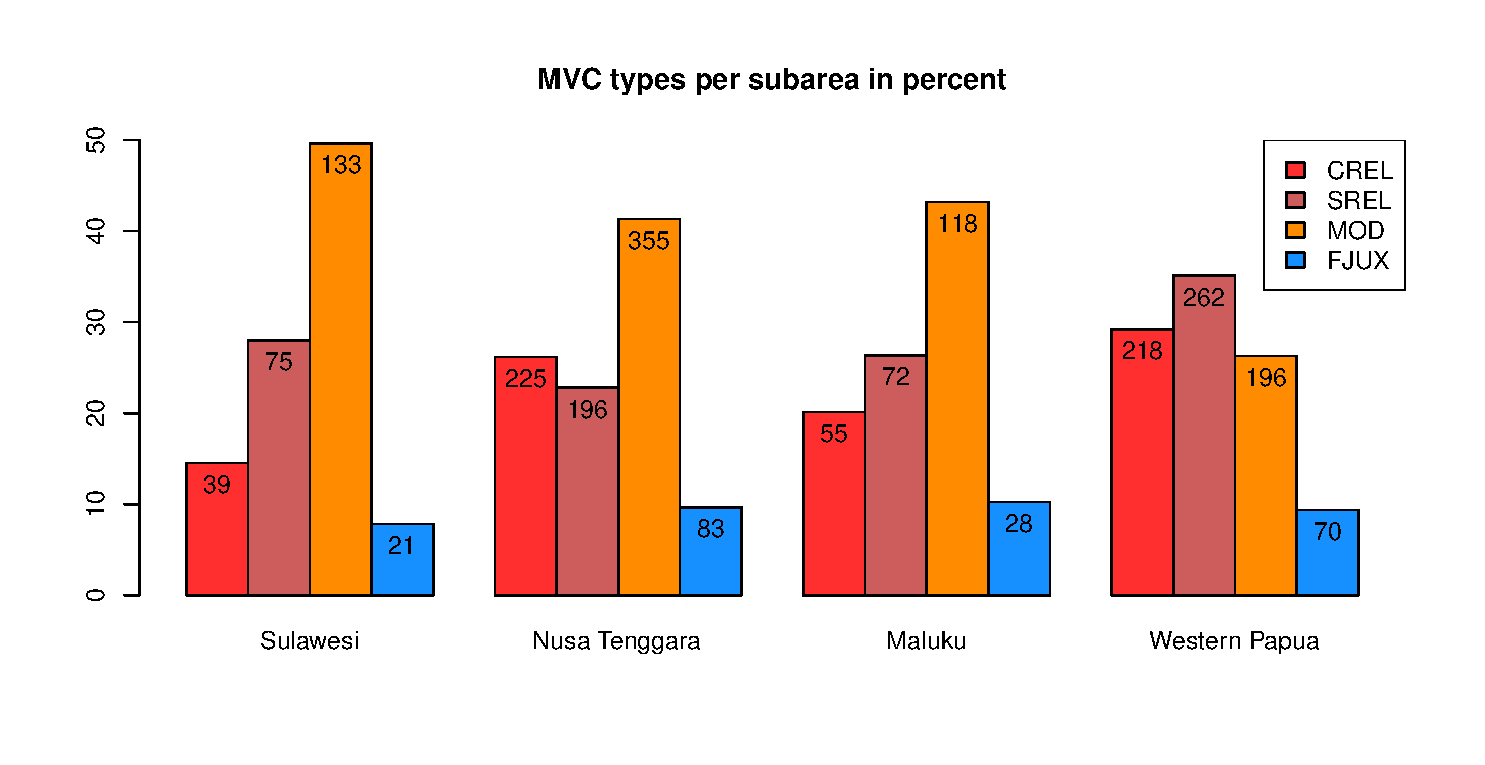
\includegraphics[width=\columnwidth]{figures/Type_Group.eps}
\caption[MVC types per subarea in percent]{MVC types per subarea in percent. \textsc{crel} = component-relating constructions, \textsc{srel} = stage-relating constructions, \textsc{mod} = modifying constructions, \textsc{fjux} = free juxtaposition constructions. Numbers on top of the bars refer to the number of observations.}\label{fig:type-group6}
\end{figure}

The general trend from Figure \ref{fig:type-family} is mirrored in Figure \ref{fig:type-group6} on MVC types per subarea though the ratio is subject to some variation between the subareas. If we just focus on the three western subareas, \textsc{sul}, \textsc{nus}, and \textsc{mal}, a prevalence of modifying constructions is observable, with a peak of almost 50\% in the Sulawesi group. This seems suprising, given that the most prototypical modifying MVCs need to result from a considerable time span of grammaticalisation (think for instance of case-marking MVCs such as give/for, take/with and so on). Thus it would appear that Sulawesi as a subarea is not peripheral in terms of feature innovation. However, as Table \ref{table:MVCperlang} reveals, the geographically peripheral status of Sulawesi seems to be confirmed by the per language data since there is a sharp split between the northern group (Pendau and Tajio), and the south-eastern group (Tolaki, Muna, and Tukang Besi). It is only in the latter group that modifying constructions indeed score highest. Both Pendau and Tajio have \textsc{mod} constructions to a much lesser extent, with motion constructions from the \textsc{crel} and \textsc{srel} families prevailing instead. The south-eastern languages, on the other hand, only exhibit weak signs of \textsc{crel} use.

The Western Papua group deviates furthest from the overall MVC type ratio. Modifying constructions are less preferred than both \textsc{crel}s and \textsc{srel}s. Stage-relating constructions do especially well with about 35\% of all instances. What remains stable across all four subgroups is the low percentage of recorded \textsc{fjux} constructions.

\begin{table}
\begin{footnotesize}
\begin{tabular}{lrrrr}
  \lsptoprule
 & CREL & SREL & MOD & FJUX \\ 
  \hline
  Muna &   6 &   2 &  32  &   10  \\ 
  Pendau &  26 &  19 &   5  &   1  \\ 
  Tajio &   4 &  18 &   6  &   4  \\ 
  Tolaki &   3 &  20 &  40  &   2  \\ 
  Tukang Besi &   0 &  16 &  50   &   4 \\ \hline 
  Abui &  10 &  20 &  73  &   6  \\ 
  Alorese &  23 &  17 &   4  &   3  \\ 
  Bunaq &  23 &   6 &  55  &   3  \\ 
  Kaera &  9 &   10 &  4  &   1  \\ 
  Kambera &  15 &   2 &  24  &   3  \\ 
  Klon &  28 &  25 &  40  &   7  \\ 
  Makalero &  17 &   9 &  48  &   2  \\ 
  Teiwa &   18 &  29 &  17  &   21  \\ 
  Tetun &  25 &  19 &  26  &   3  \\ 
  Waima'a &  47 &  44 &  52  &  33  \\ 
  Western Pantar &  10 &  15 &  12  &   1  \\ \hline
  Buru & 10 & 21 & 33 & 4 \\
  Selaru &   3 &   2 &   17  &   2  \\ 
  Taba &   2 &  18 &  22  &   2  \\ 
  Tidore & 33 & 23 & 23 & 13 \\
  Tobelo &   7 &   8 &  23  &   6  \\ \hline
  Abun &  13 &  15 &   1  &   4  \\ 
  Biak &  18 &  31 &  16  &   2  \\ 
  Dusner &  18 &  17 &   9  &  5 \\ 
  Hatam &  18 &  23 &   6  &   2  \\ 
  Inanwatan &  11 &   6 &   4  &   7  \\ 
  Maybrat &  18 &  21 &  30  &   9  \\ 
  Mor &  35 &  23 &   7  &   6  \\ 
  Moskona &   5 &  30 &  38  &   6  \\ 
  Mpur &  15 &  14 &  16  &  17  \\ 
  Sougb &   11 &  19 &   3  &   7 \\ 
  Wooi &  56 &  63 &  66  &   5  \\ 
   \hline
   Total & 537 & 605 & 802 & 202 \\
   \lspbottomrule
\end{tabular}
\end{footnotesize}
\caption[Distribution of attested MVC types per language]{Distribution of attested MVC types per language.}
\label{table:MVCperlang}
\end{table}

Table \ref{table:MVCperlang} gives the numbers of MVC types per language. All languages seem to make use of all four constructional families, with the exception of Tukang Besi for which no component-relating constructions could be found. Although all languages have reported instances of all construction types, different profiles are visible. Some languages, such as Abun or Alorese, show only very few cases of \textsc{mod}s. Other languages have but a few cases of \textsc{crel}s (and, to a lesser extent, \textsc{srel}s) but show a proliferation of \textsc{mod}s, like the group of south-eastern Sulawesi languages already mentioned. Still other languages, such as the two corpus languages Waima'a and Wooi, seem to make good use of all construction families (although \textsc{fjux} scores very low in Wooi). 

Summing up, it is evident that all four techniques of MVC formation are in use all across EI. The factors that may explain the variation in the ratio of MVC types seen above will only become clear if we take a closer look at how the different constructions are distributed across the language sample. Therefore, I will turn to the four MVC families in the remainder of this chapter, providing examples of the different constructions that I assume to be associated with them, and exploring the patterns of use that can be unearthed from the data sample.

\section{Component-relating constructions}\label{sec:crel}

The notion of component here relates to verb strings in which each verb contributes part of the overall semantic structure of the MVC. This is meant to exclude other types of MVCs where the verbs do not enter into a merging relation, i.e. their LS do not undergo a feature matching process. The term component should therefore not be confused with other uses in the literature. For instance, \citet{dixon2006serial} seems to use the term component verb to refer to any verb that takes part in a serialisation construction. Another conflicting use of the term is the distinction into component vs. narrative SVCs by \citet{vanstaden2008serial}. It is based upon the notion of `macro event' introduced by \citet{talmy2000toward} and formally elaborated into a testable category by \citet{bohnemeyer2007principles, bohnemeyer2011}. A construction is said to be `component-relating' when it ``compose[s] so-called `macro-events’
out of smaller units that we refer to as `subevents’", and it is called `narrative' when it ``compose[s] larger event complexes out of macro events" \citep[28]{vanstaden2008serial}. Thus the definition of componentiality is essentially derived from an event-based account. 

Componential in my sense of the term only pertains to the features that are present in a set of related constructions throughout the EI languages, specifically these: (i) both (all) verbs belong to the same lexical field (which presupposes in my approach at least a partially identical make-up of LS's), (ii) having a LS that is (partially) identical, the verbs merge part of their features, (iii) if features are overwritten in the merging process, it is features of V$_{1}$ that are preserved and features of V$_{\textsc{fin}}$ that are overwritten. From the criteria previously discussed it has become clear that both \textsc{crel} and \textsc{mod} constructions appear to possess the macro-event property (MEP) as defined by \citet{bohnemeyer2007principles}. This is indicated by the fact that these construction types do not allow for partial temporal modification. Hence, while I motivate this constraint by assuming differences in the assignment of hidden event arguments, my understanding of `component-relating' is quite similar to van Staden and Reesink's `component SVCs'. Specifically, I share their insight that among serialisation constructions there are cases that are conceptually packed rather closely while other constructions have parts that behave more like independent subunits.

In the last chapter, I presented an approach to motivate merging of verbal features in a MVC by proposing a set of sublexical structures that might be shared. In order to enable structural merging between verbs of the same lexical field, I introduced empty class predicates \textbf{move'} for motion verbs and \textbf{say'} for speech act verbs. In principle, this approach could be extended to any combination of verbs from identical classes, but as far as I can see it is only motion and speech verbs that behave this way in the EI sample (with a handful of potential further combinations, see §\ref{sec:other}). 

In what follows, I will quickly preview the different \textsc{crel} constructions found in the EI area, followed by a look at their distribution across the dataset. The subsequent section will then introduce the respective constructions in more detail, and present examples from the sample. Motion \textsc{crel}s appear in different construals. The most basic construal is motion complex MVCs where a motion verb in V$_1$ (most typically a manner of motion verb) is complemented by a path or ground-denoting verb in V$_2$. This is the standard pattern of feature merging that I  proposed in §\ref{sec:merging} to be the underlying semantic process in \textsc{crel} formation. Several related construals of complex motion seem to have been derived from this pattern. In \textsc{transport complex} MVCs, V$_1$ is a transitive verb of transport. In \textsc{direction complex} MVCs, V$_1$ is also transitive, but does not denote translational motion anymore. Rather, what is denoted is a movement verb to which V$_2$ adds path semantics. \textsc{Sequitive complex} MVCs have a \textsc{follow} verb in V$_1$. What all these constructions have in common is that some kind of \emph{movement} is involved, be it translational motion proper or movement of manipulated objects along some path.

Two more groups of \textsc{crel}s are found in the EI region that are not related to movement. A \textsc{speech act complex} connects a speech act verb in V$_1$ to a \textsc{say} verb in V$_2$ introducing a propositional argument (what is said). The last group comprises some odd outliers that seem to involve feature merging yet are so infrequent throughout the sample that no distribution can be traced.

\begin{sidewaystable}
\begin{tabular}{lrrrr|rr}
  \lsptoprule
& \multicolumn{4}{c}{movement} & & \\
 & {motion} & {direction} & {transport} & {sequitive} & {speech act} & {other}\\  
  \hline
  Austronesian & 166 & 46 & 47 & 9 & 20 & 3 \tabularnewline
  Papuan & 135 & 34 &  36 &  12 & 24 & 5 \tabularnewline
   \hline
  Sulawesi & 25 & 8 & 6 & 0 & 0 & 0 \tabularnewline
  Nusa Tenggara & 144 & 35 & 22 & 7 & 10 & 7 \tabularnewline
  Maluku & 26 & 11 & 4 & 3 & 11 & 0 \tabularnewline 
  Papua & 106 & 26 & 51 & 11 & 23 & 1 \tabularnewline 
\hline
Total & 301 & 83 & 80 & 21 & 44 & 8 \tabularnewline
\lspbottomrule
\end{tabular}
\caption[Distribution of \textsc{crel} types]{Distribution of \textsc{crel} types across EI. Note that both subcalculations, i.e. into language family affiliation as well as into areal subgroups, each amount to the total number of observations given in the last row.}
\label{table:CREL_overview}
\end{sidewaystable}

The impression from the previous section was that \textsc{crel} constructions occur in almost all languages, and are evenly distributed over subareas and language families. If we look more closely at the different \textsc{crel} constructions this picture changes somewhat. Table \ref{table:CREL_overview} above shows the distribution of \textsc{crel} constructions across language families and subareas. The first thing to note is that \textsc{crel} constructions involving movement figure most prominently: 485 out of 537 \textsc{crel} observations involve movement of some kind. Among this group, motion complex constructions are most often attested, making it the default \textsc{crel} construction in the EI dataset. Figures \ref{fig:crel-family} and \ref{fig:crel-group} below illustrate the ratio between \textsc{crel} constructions with regard to language affiliation and subgroup, respectively. Once more, we can discern that linguistic affiliation does not seem to bear on the use of the different constructions. It is only at the subarea level that we can observe considerable differences. The most obvious pattern is a lack of sequitive and speech act constructions in the Sulawesi subgroup. This tallies well with the assumption already mentioned that Sulwesi, forming the western periphery of an assumed Wallacea Sprachbund, does not have the full range of MVC constructions in use. The other three subareas each show all \textsc{crel} constructions, although there are more observations of the minor constructions in Maluku and Western Papua languages than in the Nusa Tenggara languages.

\begin{figure}
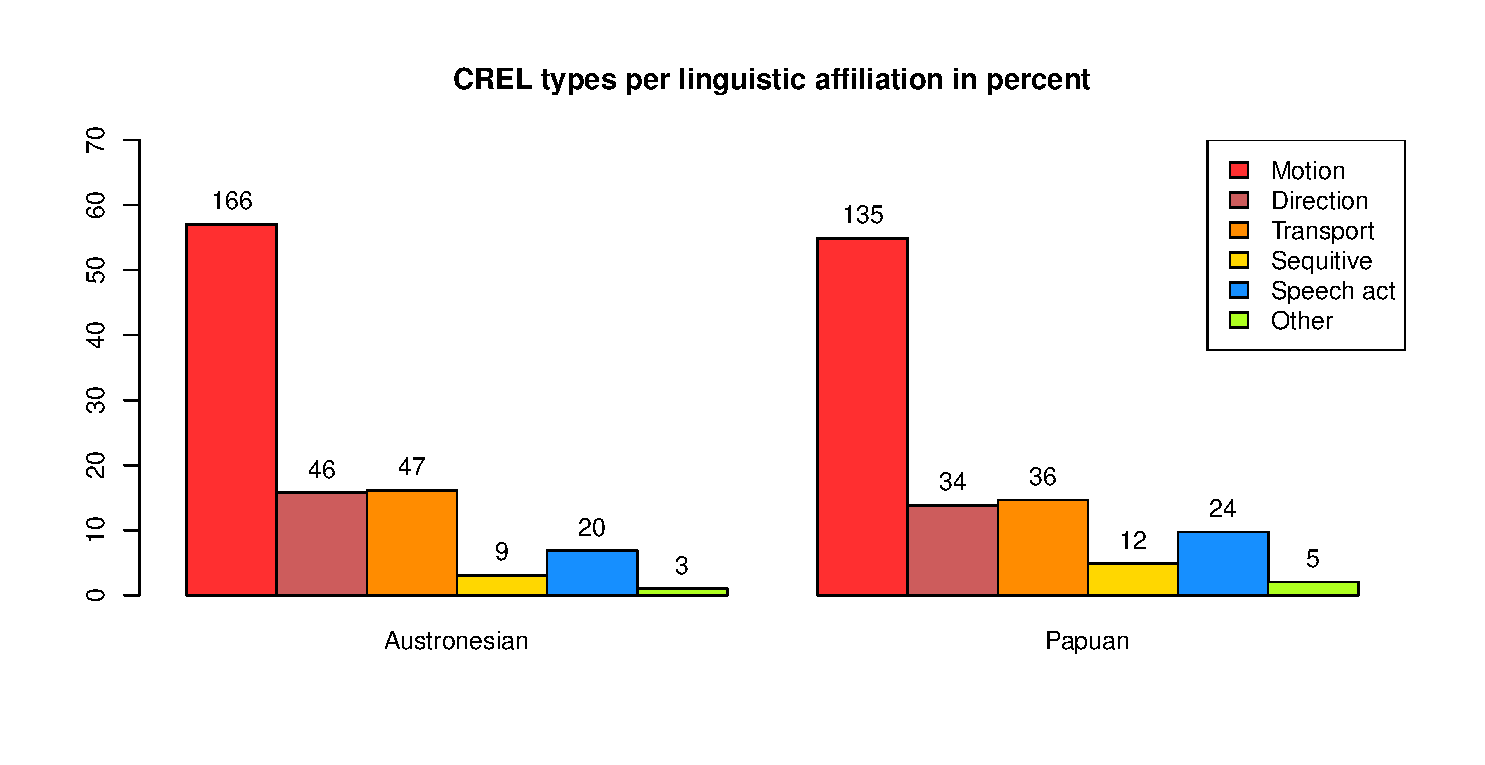
\includegraphics[width=\columnwidth]{figures/CREL_Family.eps}
\caption[CREL types per linguistic affiliation in percent]{CREL types per linguistic affiliation in percent. Numbers on top of the bars refer to the number of observations in the dataset.}\label{fig:crel-family}
\end{figure}
\begin{figure}
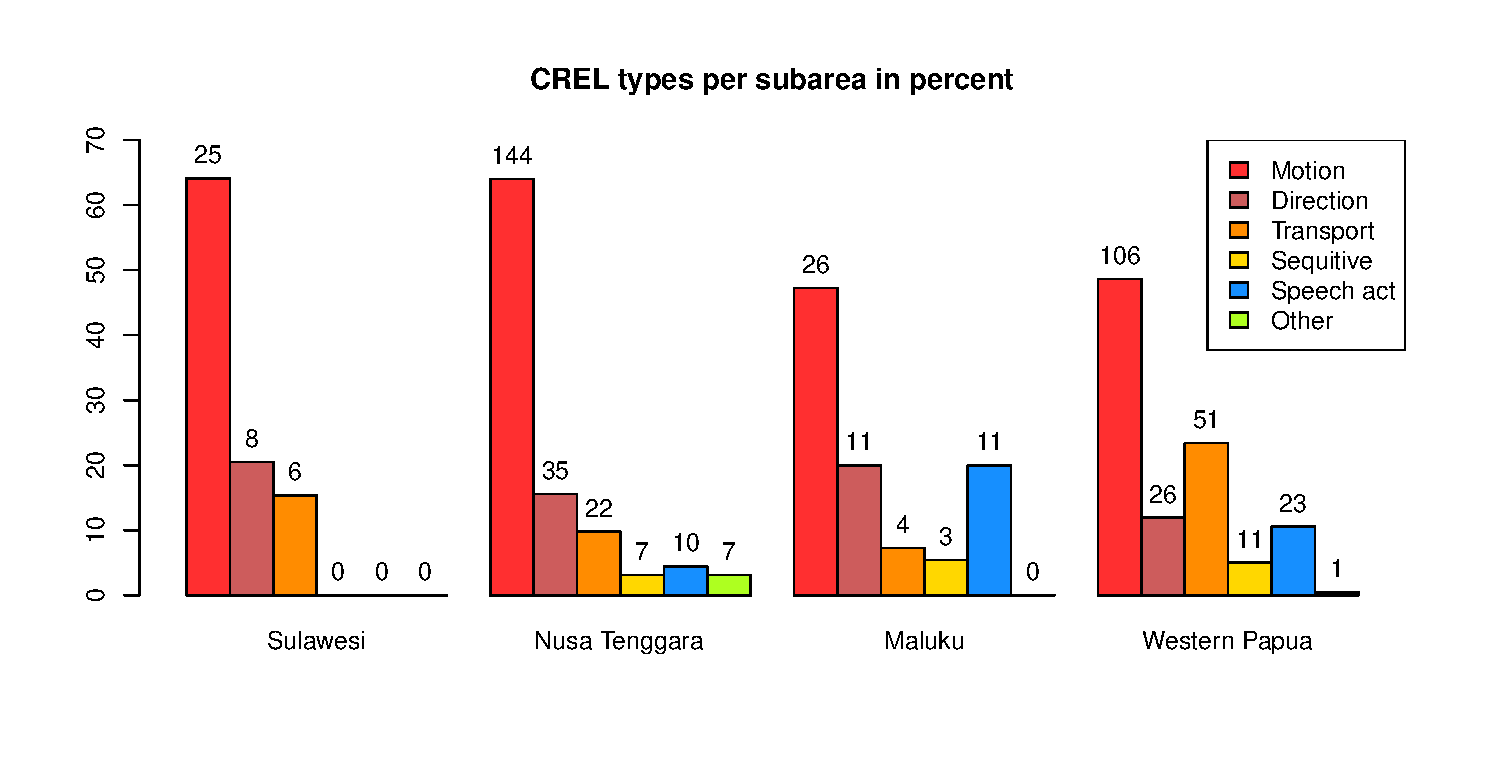
\includegraphics[width=\columnwidth]{figures/CREL_Group.eps}
\caption[CREL types per subarea in percent]{CREL types per subarea in percent. Numbers on top of the bars refer to the number of observations in the data sample.}\label{fig:crel-group}
\end{figure}

%Table \ref{table:crel_language} below shows the distribution of attested CREL construction types per language. 

The different constructions are quite evenly distributed within the four subgroups showing that they are in fact widespread throughout the subareas, and do not just cluster in some exceptional language. If a language makes use of feature merging resulting in \textsc{crel}s, there are always motion complex constructions among it. Direction, transport, and sequitive \textsc{crel}s all involve transitive verbs in V$_1$ position, and the figures for these constructions are much lower than for motion complexes. What is more, the occurrence of the 'minor' movement constructions appears to entail the use of the basic motion complex construction. That is, there are no languages for which only minor movement constructions are attested. This supports the assumption that the motion complex construction is the most basic one, possibly the construction from which the minor ones are derived. Another entailment suggested by the EI data is that if a language shows sequitive \textsc{crel}s then it also tends to have attested direction and transport \textsc{crel}s (with the exception of Inanwatan and Sougb). Direction and transport, on the other hand, seem not directly related to one another as either construction may occur without the other.

%\begin{table}
%\begin{scriptsize}
%\begin{tabular}{lrrrrrr}
%\lsptoprule
%& \multicolumn{4}{c|}{movement} & & \\
% & {motion} & {direction} & {transport} & {sequitive} & {speech act} & {other}\\ 
 % \hline
  %Muna &   5 &   0 &   1 &   0 &   0 &   0  \\ 
  %Pendau &  15 &   7 &   4 &   0 &   0 &   0 \\ 
  %Tajio &   3 &   0 &   1 &   0 &   0 &   0 \\ 
  %Tolaki &   2 &   1 &   0 &   0 &   0 &   0 \\ 
  %Tukang Besi & 0 & 0 & 0 & 0 & 0 & 0 \\ \hline
  %Abui &   4 &   3 &   1 &   2 &   0 &   0 \\ 
  %Alorese &  19 &   1 &   1 &   1 &   1 &   0 \\ %
 % Bunaq &  18 &   5 &   0 &   0 &   0 &   0 \\ 
 % Kaera &   7 &   0 &   2 &   0 &   0 &   0 \\ 
 % Kambera &   3 &   4 &   4 &   1 &   1 &   2 \\ %
  %Klon &  21 &   0 &   0 &   0 &   4 &   3 \\ 
  %Makalero &  11 &   1 &   4 &   0 &   1 & 0  \\ %
  %Teiwa &   14 &   0 &   4 &   0 &   0 &   0 \\ 
  %Tetun &  16 &   4 &   4 &   0 &   0 &   1 \\ 
  %Waima'a &  23 &  17 &   2 &   3 &   2 &   0 \\ %
  %Western Pantar &   8 &   0 &   0 &   0 &   1 &   1 \\ \hline
  %Buru & 8 & 1 & 0 & 0 & 1 & 0 \\
  %Selaru &   1 &   0 &   0 &   0 &   2 &   0 \\ 
  %Taba &   2 &   0 &   0 &   0 &   0 &   0 \\ 
  %Tidore & 13 & 9 & 4 & 3 & 4 & 0 \\
  %Tobelo &   2 &   1 &   0 &   0 &   4 &   0 \\ \hline
 % Abun &   4 &   3 &   6 &   0 &   0 &   0 \\ 
 % Biak &   9 &   3 &   5 &   1 &   0 &   0 \\ 
 % Dusner &  11 &   0 &   4 &   1 &   2 &   0 \\ 
 % Hatam &   5 &   4 &   9 &   0 &   0 &   0 \\ 
 % Inanwatan &   4 &   0 &   4 &   2 &   0 &   1 \\ 
 % Maybrat &   8 &   4 &   0 &   0 &   6 &   0 \\ %
 % Mor &  15 &   2 &   8 &   2 &   8 &   0 \\ 
 % Moskona &   4 &   0 &   1 &   0 &   0 &   0 \\ %
 % Mpur &   4 &   4 &   0 &   5 &   2 &   0 \\ 
 % Sougb &   8 &   0 &   1 &   0 &   2 &   0 \\ 
 % Wooi &  34 &   6 &  13 &   0 &   3 &   0 \\ 
 %  \hline
 %  Total & 301 & 80 & 83 & 21 & 44 & 8 \\
 %  \hline
%\end{tabular}
%\end{scriptsize}
%\caption{Distribution of attested CREL construction types per language}
%\label{table:crel_language}
%\end{table}

Now, having arrived at a MVC analysis driven by semantic interaction techniques as introduced in Chapter \ref{ch:sem}, we can bring the morphosyntactic parameters from Chapter \ref{ch:gram} back into play. Table \ref{table:crel_formal} illustrates that the \textsc{crel} constructions display a much more homogeneous picture with regard to morphosyntactic properties than has been found for the whole sample in Chapter \ref{ch:gram}. In terms of referentiality, the same-subject configuration is strongly prevalent in all \textsc{crel} constructions, except for direction complexes. This does not come as a surprise, given that in direction complexes, there is typically an argument-switch involved (see discussion below in §\ref{sec:direction}). This variation in referentiality encoding correlates with a tendency of direction complexes (as well as the other movement constructions) towards inflecting only the starting verb of the series. Uninflected V$_2$ in direction complexes thus leads to some degree of coding ambiguity with regard to argument interaction. This helps explain the wide range of referentiality values annotated.

The headedness patterns from Table \ref{table:crel_formal} point out another notable tendency. In all movement constructions it is V$_1$ that is allocated the main inflectional load. The ``1" inflection pattern is predominant across the board, and outnumbers the ``B" pattern. Associating information on verbal categories, such as TAM or subject indexing, to only one head creates an asymmetry that can be interpreted as lending prominence to V$_1$. This is basically in line with the criterion introduced in §\ref{sec:criteria_mvcs} above, namely that in \textsc{crel} it is V$_1$ that preserves its verbal properties rather than the subsequent verbs\footnote{Note that these figures are slightly biased towards the ``1" pattern as I interpreted directional verboids in post-verbal position as verbs, for instance in languages that I am familiar with (Wooi, Waima'a) or where the lexeme in question can either diachronically or synchronically be traced back to a verb root (think of Wooi \textit{ma} from the very first example in Chapter \ref{ch:introduction}). Alternative analyses might reanalyse some such strings into verb - (directional) particle constructions, and arrive at lower numbers of ``1" patterns.}. This prominence shift is, however, not visible in speech complex constructions, as these appear to favour the ``B" pattern.

\begin{table}
\centering
\begin{tabular}{rrrrrr}
  \lsptoprule
Referentiality & S & SO & D & A & E \\ 
  \hline
motion complex & 300 &   0 &   0 &   0 &   1 \\ 
  direction complex &  20 &   5 &  33 &   0 &  22 \\ 
  transport complex &  80 &   0 &   2 &   1 &   0 \\ 
  sequitive complex &  19 &   0 &   2 &   0 &   0 \\ 
  speech act complex &  44 &   0 &   0 &   0 &   0 \\ 
  other &   8 &   0 &   0 &   0 &   0 \\ 
   \hline
 \\
  \hline
Headedness & B & 1 & 2 & S & N \\ 
  \hline
motion complex &  39 &  83 &   2 &  10 &  14 \\ 
  direction complex &  12 &  22 &   0 &   5 &   6 \\ 
  transport complex &  15 &  32 &   4 &   4 &   4 \\ 
  sequitive complex &   3 &   6 &   2 &   2 &   2 \\ 
  speech act complex &  24 &   4 &   1 &   1 &   4 \\ 
  other &   0 &   0 &   1 &   2 &   0 \\ 
   \hline
 \\
  \hline
Contiguity & W & C & 1 & 2 & 3 \\ 
  \hline
motion complex &   8 & 241 &  46 &   5 &   1 \\ 
  direction complex &   0 &  54 &  24 &   2 &   0 \\ 
  transport complex &   4 &  47 &  31 &   0 &   1 \\ 
  sequitive complex &   2 &  17 &   2 &   0 &   0 \\ 
  speech act complex &   0 &  34 &  10 &   0 &   0 \\ 
  other &   1 &   7 &   0 &   0 &   0 \\ 
   \lspbottomrule
\end{tabular}
\caption[Morphosyntactic properties of \textsc{crel} constructions]{Morphosyntactic properties of \textsc{crel} constructions in EI. Table components from top to bottom refer to referentiality (see §\ref{sec:argumentstructure}), headedness (see \ref{sec:headedness}), and contiguity (see \ref{sec:contiguity}), respectively.}
\label{table:crel_formal}
\end{table}

In the following sections, I will briefly present the \textsc{crel} constructions one by one. The purpose of these sections is to provide examples from all subareas where the construction is attested.

\subsection{Motion complex} \label{sec:motioncomplex}

Motion complex constructions form the largest subgroup of the \textsc{crel} class with 301 attested data points out of 537 instances of \textsc{crel}s and 2146 instances of MVCs in total. The basic distributional properties are the same as for the \textsc{crel}s in general, since every language in the sample that has \textsc{crel} constructions also has motion complexes. Table \ref{table:basiccrelmotion} gives the respective numbers as well as the general template. A motion complex is made up of two or more verbs with each verb belonging to the lexical field of motion verbs.

\begin{table}
\begin{tabular}{ll}
\lsptoprule
Feature&Value\tabularnewline
\hline
Template&V1 \textsc{motion} -- V2 \textsc{motion}\tabularnewline
No. of attested instances& 301/2146 \tabularnewline
No. of attested languages& 31/32 (not attested: Tukang Besi) \tabularnewline
Distribution across areas& \textsc{sul} (4/5), \textsc{nus} (11/11), \textsc{mal} (5/5), \textsc{pap} (11/11) \tabularnewline
Distribution across families& \textsc{pap} (16), \textsc{aus} (15) \tabularnewline
\lspbottomrule
\end{tabular}
\caption[Template and basic distribution of \textsc{crel} motion complexes]{Template and basic distribution of \textsc{crel} motion complexes in the EI sample. First verb mostly intransitive with few exceptions, second verb intransitive or transitive}
\label{table:basiccrelmotion}
\end{table}

The following examples (\ref{Pendau24}) to (\ref{Hatam001}) are from all four subareas, and show the typical appearance of motion complexes in EI. The first verb tends to be intransitive (with only a handful of exceptions, for instance \textsc{leave}, \textsc{cross}, or \textsc{reach} verbs taking a ground argument) and often refers to the way the motion is carried out, or gives part of the path information needed to project the whole motion vector. The verb in V$_{\textsc{fin}}$ is most often a path verb. In the Pendau example (\ref{Pendau24}) the moving referent undergoes a non-volitional motion event on a vertical projection plane. Example (\ref{Alorese001}) from Alorese shows a manner of motion verb followed again by a path verb, this time opening up a deictic vector directed towards the speaker origo. This example is somewhat unusual in that the moving referent is inanimate (most cases have animate actors performing some motion at will). The next example has another common combination of motion verbs with a reverse path verb in V$_{2}$ position and a vertical path verb in V$_{1}$. Note that the sample also contains motion complexes with exactly the opposite order where a \textsc{return} verb is followed by a vertical or horizontal path verb. These cases are, however, restricted to combinations of motion verbs that both convey path semantics. Non-path-denoting motion verbs never appear in V$_1$, supporting the assumption that manner is placed before path in a motion complex. The last example from Hatam has a potentially transitive ground-denoting verb in V$_{1}$ which, however, need not be produced with a ground NP. In such cases like (\ref{Hatam001}) I interpret the function of contained path verbs (\textsc{enter}, \textsc{exit}) as emphasizing additional information on the path rather than introducing a ground referent which is not overtly specified.

\ea \label{Pendau24}
\langinfo{Pendau}{Austronesian, WMP}{\citealt[344]{Quick2007}}\\
\glll odo moo nanabumo manyau rilalong nuapi \\
odo moo no-nabu=mo ma-nyau ri=lalong nu=api \\
monkey this \textsc{st}.\textsc{rls}-fall=\textsc{compl} \textsc{irr}-go.down \textsc{loc}=inside \textsc{cn}=fire \\
\glft `This monkey fell down into the fire.' \\ 
\z

\ea \label{Alorese001}
\langinfo{Alorese}{Austronesian, CMP}{\citealt[63]{klamer2011alorese}}\\
\gll terus, kaju fatang nepi mene \\
then wood sea float come \\
\glft `Then a piece of wood came floating (towards us).'\\ 
\z

\ea \label{Taba002}
\langinfo{Taba}{Austronesian, SHWNG}{\citealt[295]{bowden2001taba}}\\
\glll ncopang nmul hu \\
n=sopang n=mul hu \\
\textsc{3}\textsc{sg}=descend \textsc{3}\textsc{sg}=return \textsc{cont} \\
\glft `(S)he's still coming back down.'\\ 
\z

\ea \label{Hatam001}
\langinfo{Hatam}{Papuan, Hatam-Mansim}{\citealt[100]{reesink1999grammar}}\\
\gll a-coi kwei \\
\textsc{2}\textsc{sg}-enter come \\
\glft `Come in.' (= invitation to visitor)\\ 
\z

The four examples are also typical motion complexes in terms of their morphosyntactic behaviour, as we have already seen from Table \ref{table:crel_formal}. \textsc{crel} motion complexes can basically appear in all inflection patterns. This is reflected by the examples: in (\ref{Pendau24}) and (\ref{Taba002}) both verbs take inflectional marking\footnote{The Sulawesi case is a bit more complex inasmuch as a small group of motion verbs in V$_{\textsc{fin}}$ shows defective inflectional behaviour. In Pendau, only \textit{nyau} can occur with a prefix, either taking the form \textit{ma-nyau} or \textit{menyau} (from \textit{M-pe-nyau} \textsc{irr}-\textsc{sf/dyn}-go.down; see ex. (55) in \citealt[342]{Quick2007} and discussion on p.344 incl. footnote 8). As Quick's examples and discussion show, there is no realis form that would match \textsc{irr} \textit{ma-nyau}. A similar form occurs in neighbouring Tajio with \textit{minyau} which could be analysed as a lexicalised former irrealis form. However, contemporary Tajio also lacks a realis counterpart (see \citealt[136]{mayani2013grammar}).}, example (\ref{Hatam001}) shows inflection only on the first verb, and in Alorese (\ref{Alorese001}) both verbs remain bare. The choice of inflection pattern is influenced by two factors: (i) the overall grammatical system of the language, and (ii) dominance of the first verb. I assume that the first factor is a relative one that is particularly influential in areas with high levels of mutual linguistic contact. The second factor seems to be a more general characteristic of motion verb construals in the EI area, and draws supporting evidence from two facts. First, as noted earlier, in feature merging it is features of V1 that are preserved (\textsc{fall} in V$_{1}$ passes on features of non-volitionality while \textsc{fall} in V$_{\textsc{fin}}$ does not). Second, the diachronic development in motion verb construals seems to suggest a gradual decline of verbal properties in V$_{\textsc{fin}}$, leading to the eventual loss of inflection and the ultimate formation of a class of directional operators. This process is well-known from many languages (see for instance \citealt[31]{Aikhenvald2006}).

Inanwatan is the only language in the sample that really seems to have developed a motion construction in which the second verb bears the morphosyntactic locus. Consider the following two examples.

\ea \label{Inanwatan16}
\langinfo{Inanwatan}{Papuan, SBH}{\citealt[49]{devries2004}}\\
\gll mé-se-i ewáiwa nóe-we-i-di \\
\textsc{3}\textsc{sbj}-walk-\textsc{pst}.\textsc{m} and go.out-\textsc{3}\textsc{sbj}-descend-\textsc{pst}.\textsc{m} \\
\glft `(And) he went on and on and he arrived.'\\ 
\z

\ea \label{Inanwatan20}
\langinfo{Inanwatan}{Papuan, SBH}{\citealt[55f.]{devries2004}}\\
\gll mé-de-wo-i ewáiwa \\
\textsc{3}\textsc{sbj}-go.across-come-\textsc{pst}.\textsc{sg}.\textsc{m} and \\
\glft `He came across and [...]'\\ 
\z

The first example in (\ref{Inanwatan16}) depicts the construction that I coded as ``2": the first motion verb, \textit{noé} `go out', is preposed to the finite verb complex, \textit{we-i-di} `he descended', as a bare stem. Another pattern, where both verbs share the inflection set of prefix and suffix, is illustrated in (\ref{Inanwatan20}). Here, both motion verbs can be conceived as inflected (`shared' inflection in my terms). The fact that Inanwatan affords two different construals of motion complexes could indicate that the deictic path verb \textit{wo} `come' (and maybe others more in this construction) has already begun to lose part of its verbal properties in this context, moving along a grammaticalisation path that ultimately leads to the formation of a class of non-verbal directional elements. Inanwatan \textit{wo} would thus generally fit into the pattern of deverbalisation of \textsc{go} and \textsc{come} verbs in many EI languages.

Two languages in the \textsc{pap} subarea, Inanwatan and Sougb, allow motion complex construals within one phonological word. The Inanwatan examples (\ref{Inanwatan16}) and (\ref{Inanwatan20}) above have already illustrated this type and the figures for Inanwatan indicate that the construction pattern seems the only choice for motion complex construals in that language. Sougb is a bit different as it belongs to the group of languages with more than one attested contiguity value. The reason for this is that Sougb \textit{da} (from \textit{eda} `go') and \textit{in} (from \textit{en} `come'), the only two motion verbs attested in V$_{\textsc{fin}}$, behave like clitics: they seem to attach to V$_{1}$ unless a direct object NP or a goal NP intervenes in which case they attach to the NP. Note, however, that the source PP in (\ref{Sougb002a}) does not attract the clitic verb. The Sougb case is illustrated by the following examples:

\ea \label{Sougb002a}
\langinfo{Sougb}{Papuan, EBH}{\citealt[200]{reesink2002grammar}}\\
\gll godeh hom g-ougb-da dau m-ena \\
child one \textsc{nom}-run-go from \textsc{3}\textsc{sg}-father \\
\glft `A son who ran away from his father.' \\ 
\z

\ea
\langinfo{Sougb}{Papuan, EBH}{\citealt[226]{reesink2002grammar}}\\
\gll yen y-aiga duhu-da \\ 
you \textsc{2}\textsc{pl}-cross water-go \\
\glft `Cross the river.'\\ 
\z

\ea
\langinfo{Sougb}{Papuan, EBH}{\citealt[226]{reesink2002grammar}}\\
\gll en esogw-esa se duhu aud en-da \\ 
he jump-stand at water to him-go \\
\glft `He jumped into the water towards him.'\\ 
\z
\xe

Referentiality in motion complexes remains ``S" throughout all cases, as shown in Table \ref{table:crel_formal} above. In principle, it is not clear why there are no languages that use the predicate-argument reanalysis scenario instead (in which the modifier verb takes the whole main verb predication as its argument). This pattern occurs in Southeast Sulawesi languages with construals of temporal verboids. If a temporal verboid, as shown in example (\ref{Muna018}) from Muna, can take as its subject the second VP, one might wonder why this is not also an option in motion complex MVCs, especially if the second verb is a path verb that has already lost part of its verbal properties. A construal like `it is usual (that) I swim' could then be paralleled by construals such as `it is hither I go/my going is hither'. Yet no such option is attested in the sample except for one construction in Mpur, illustrated in (\ref{Mpur061}) below.

\ea \label{Muna018}
\langinfo{Muna}{Austronesian, WMP}{\citealt[236f.]{vandenberg1989}}\\
\gll no-rea a-leni \\
\textsc{3}\textsc{sg}.\textsc{rls}-usual \textsc{1}\textsc{sg}.\textsc{rls}-swim \\
\glft `I usually swim.'\\ 
\z

\ea \label{Mpur061}
\langinfo{Mpur}{Papuan, isolate}{\citealt[101]{ode2002sketch}}\\
\gll bisa n-dokwa na n-aw a-ye' \\
can \textsc{1}\textsc{sg}-bring for \textsc{3}\textsc{sg}.\textsc{f}-run \textsc{3}\textsc{sg}.\textsc{m}-out \\
\glft `Bring (something) to get her out.'\\ 
\z

The motion complex \textit{n-aw a-ye'} here is construed as a purpose complement marked as such by \textit{na}. Mpur has overt gender distinction between masculine and feminine in third person singular. In (\ref{Mpur061}) we observe a mismatch in gender marking between the first verb and the second indicating that the subject of the outward movement denoted by \textit{ye'} cannot be the female runner from V$_{1}$. The only other interpretation that seems available here is that \textsc{3sg.m} can be used as a default marker for sentential arguments in Mpur, taking the first VP \textit{n-aw} as a subject here. Predicate-argument reanalysis is a feature that is further attested in the Bird's Head area, for instance in argument-marking constructions from Maybrat, in sequentialiser constructions from Moi (not part of the sample), or manner serialisation in Moskona where the zero-marked manner verb is interpreted to take the entire predicate of the main verb as its subject \citep[299f.]{gravelle2010grammar}. 

Summarising so far, we have seen that despite the large amount of data points from almost all EI languages, motion complexes are moulded into a fairly consistent form. From a formal perspective we can state that the verbs tend to stand adjacent to each other and display co-referential participant marking ('same subject'). If there is verbal inflection then it is the first verb that tends to receive it except for the \textsc{nus} subarea where constructions (and languages) without clear inflection patterns predominate. From a semantic viewpoint, the stable factor is that the verbs all belong to the lexical field of motion verbs and merge part of their LS. The bulk of constructions has the following order: V$_{1}$ refers to the act of moving (predominantly lexicalised manner of motion) while V$_{\textsc{fin}}$ contributes information on the way the motion event unfolds through space and time. Yet, we have already seen other examples (e.g. the Inanwatan examples in (\ref{Inanwatan16})) where V$_{1}$ presents path information and/or introduces (covert) ground referents (`go.out', `go.across') which the motion event is set in relation to. This suggests that there is a good deal of variation as to which motion verb class appears in which constructional slots, in particular when language-specific constituent order constraints (as AOV in Inanwatan) clashes with the order dominant verb - modifier verb in motion complexes. The most crucial ordering principle, however, that I take to be at the heart of motion complex constructions, \textsc{manner} before \textsc{path}, is well-attested and not subject to any change in order. This constraint offers an interesting perspective on the framing discussion in complex motion expressions (as already briefly mentioned in §\ref{sec:sem-templates}). Talmy's two-way typology \citep{talmy1985lexicalization, talmy2000toward} has recently been expanded into a three-way typology, accomodating serialising languages as an independent framing type (called equipollently-framed by \citealt{slobin2004many}). While the nature of motion framing in SVCs is still under discussion, it is quite remarkable that both satellite-framed and serialising languages show a strong preference to place \textsc{manner} before \textsc{path} (see \citealt{Ameka2013} for a recent overview).

\subsection{Direction complex} \label{sec:direction}
Direction complexes bear a resemblance to motion complexes as well as to transport complexes. With both construction types they share the (predominant) use of motion path verbs in V$_{\textsc{fin}}$ defining a trajectory of the motion event. Another feature they share with transport complexes is that the first verb in a direction complex is in most cases transitive (only directed perception verbs such as \textsc{look} deviate from this pattern). They differ, however, from both previous construction types in that the motion event is no longer understood as translational motion but as a derived motion concept, capturing body part movement as well as stimulus perception vectors. Table \ref{table:basiccreldir} has the basic features of direction complexes in the EI area.

\begin{table}
\begin{tabular}{ll}
\lsptoprule
Feature&Value\tabularnewline
\hline
Template&V1 \textsc{action/perception$_{\textsc{tr}}$} - V2 \textsc{motion$_\textsc{intr}$}\tabularnewline
No. of attested instances& 80/2146 \tabularnewline
No. of attested languages& 19/32 \tabularnewline
Distribution across areas& \textsc{sul} (2/5), \textsc{nus} (7/11), \textsc{mal} (3/5), \textsc{pap} (7/11) \tabularnewline
Distribution across families& \textsc{pap} (9), \textsc{aus} (10) \tabularnewline
\lspbottomrule
\end{tabular}
\caption[Template and basic distribution of \textsc{crel} direction complexes]{Template and basic distribution of \textsc{crel} direction complexes in the EI data sample. First verb denotes object manipulation/relocation or perception, second verb contributes motion path semantics.}
\label{table:basiccreldir}
\end{table}


The following examples present typical cases of direction complexes from the \textsc{sul}, \textsc{nus}, and \textsc{pap} subareas (the only example from \textsc{mal} will be discussed further below). All three of them make use of a vertical or deictic path verb in V$_{\textsc{fin}}$, yet the event does not encode translational motion of the actor. In (\ref{Pendau027}) the path verb \textit{manyau} denotes a downward trajectory of some instrument. Pendau is the only \textsc{sul} language with several cases of attested direction complexes, both in combination with verbs of object manipulation ('cast', 'slash') and with perception verbs ('stare', 'look'). Example (\ref{Abui061}) from Abui illustrates a directed perception event where the vertical path verb \textit{mara} adds the vector that spans between the experiencer (introduced here by grammaticalized \textit{ng} 'see') and his visual focus. Again it is the constructional setting that pre-empts the motion verb from being interpreted as an act of literal motion. The last example is from the \textsc{pap} subarea and shows yet another way of combining an action verb with a motion path verb. \textit{tu} is a verb of object relocation rather than object manipulation but serves well in a direction complex. Other examples from Maybrat involve the verb \textit{ai} 'hit'.

\ea \label{Pendau027}
\langinfo{Pendau}{Austronesian, WMP}{\citealt[346]{Quick2007}}\\
\glll nitoto'a'onyo manyau riba'i nirapinyo \\
ni-toto'-a'=nyo ma-nyau ri=ba'i ni=rapi=nyo \\
\textsc{iv}.\textsc{rls}-slash-\textsc{tr}=\textsc{3}\textsc{sg}.\textsc{gen} \textsc{ug}.\textsc{irr}-go.down \textsc{loc}=head \textsc{pn}.\textsc{gen}=spouse=\textsc{3}\textsc{sg}.\textsc{gen} \\
\glft `He slashed it down into his wife's head.' \\ 
\z

\ea \label{Abui061}
\langinfo{Abui}{Papuan, TAP}{\citealt[363]{kratochvil2007grammar}}\\
\gll di=ng wahai mara \\
\textsc{3}\textsc{act}=see look go.up.\textsc{cont} \\
\glft ‘He looks up.’\\ 
\z
\xe

\ea \label{Maybrat102}
\langinfo{Maybrat}{Papuan, isolate}{\citealt[215]{dol2007grammar}}\\
\gll t-tu aya m-amo cerek a \\
\textsc{1}\textsc{sg}-pour water \textsc{3}\textsc{u}-go thermos.flask \textsc{q} \\
\glft `Should I pour water into the thermos flask?'\\ 
\z

The last example from Maybrat is reminiscent of ambient serialisation inasmuch as the referential alignment shows a mismatch between the subject of V$_{1}$ and V$_{\textsc{fin}}$. Dol explicitly discusses this construction as a shared argument construction and interprets the object of V$_{1}$ as subject of V$_{\textsc{fin}}$ \citep[217]{dol2007grammar}, that is, it is the water that `goes' into the thermos flask not the pouring of the water as would be the case with ambient marking. 

One distributional property of direction complex constructions that is particularily striking is that all instances of direction complexes encoded as double-head inflection (``B" pattern) only feature verbs of object manipulation or relocation. There is not a single instance of double marking with perception constructions. This raises the following question: what is the (understood) subject of the motion path verb in V$_{\textsc{fin}}$? Is it the experiencer, the stimulus (with transitive perception verbs), the whole predication of perceiving something, or maybe none at all as the motion verbs might have already lost part of their verbhood in that particular construction? An analysis of the EI sample shows that all languages that have both types (action and perception) attested either do not use verbal inflection at all (Alorese, Waima'a), or inflect the initial verb only (Biak, Wooi), or have unregular inflection patterns not generally suitable for characterising constructions (Pendau, Abui). Therefore we cannot at this point make any prediction on the identity of the second subject argument in direction complexes. Another feature that becomes evident is that all languages that allow for perceptional direction complexes are in fact Austronesian languages (except for the one example from Abui illustrated in (\ref{Abui061}) above). If this tendency proved to be true with more data, one could state that direction complexes of the perception type are more common in Austronesian than in Papuan languages. On the other hand might a closer inspection of larger amounts of data generally reveal more languages with both constructions. This is foreshadowed by the fact that in both corpus languages for which more data have been collected, Waima'a and Wooi, both constructions were found to be present.

A final example that I want to present here is the (only) one from Tobelo. 

\ea \label{Tobelo033}
\langinfo{Tobelo}{Papuan, NH}{\citealt[63]{holton2003tobelo}}\\
\gll t-a-ika t-i-tauru no-maoko la no-ma-tagi \\
\textsc{1}-\textsc{vf}-\textsc{all} \textsc{1}-\textsc{3}\textsc{m}-pull \textsc{2}-stand \textsc{conj} \textsc{2}-\textsc{refl}-walk \\
\glft `I pulled him up so that he could walk.' \\ 
\z

This example is unusual in at least two ways (ignoring the resultant phase denoted by the third verb \textit{no-maoko}): first, the order action verb - motion path verb is reversed, a pattern that we do not find in the other languages. And second, the motion path verb seems to be grammatical in nature rather than a full lexical item (capable of predicating a simplex predicate). Such instances at best constitute peripheral cases of direction complexes, if at all.

\subsection{Transport complex} \label{sec:transport}

The next subtype of \textsc{crel} constructions consists of a verb of transport, such as \textsc{bring}, \textsc{hold}, \textsc{carry}, or \textsc{bear}, which is complemented by a motion path verb in V$_2$. The combination of verbs is interpreted as denoting an act of translational motion where the actor is in possession of an object and relocates it by way of changing his/her position in the landscape of discourse. Table \ref{table:basiccreltransport} lists the basic properties of transport complexes in the EI languages. 

\begin{table}
\begin{tabular}{ll}
\lsptoprule
Feature&Value\tabularnewline
\hline
Template&V1 \textsc{transport$_{\textsc{tr}}$} * V2 \textsc{motion}\tabularnewline
No. of attested instances& 83/2146 \tabularnewline
No. of attested languages& 21/32 \tabularnewline
Distribution across areas& \textsc{sul} (3/5), \textsc{nus} (8/11), \textsc{mal} (1/5), \textsc{pap} (9/11) \tabularnewline
Distribution across families& \textsc{pap} (11), \textsc{aus} (10) \tabularnewline
\lspbottomrule
\end{tabular}
\caption[Template and basic distribution of \textsc{crel} transport complexes]{Template and basic distribution of \textsc{crel} transport complexes in the EI sample. The first verb encodes possession and motion, the second verb contributes further motion components (predominantly path). The asterisk indicates that the order transport - motion is reversed in a small number of constructions}
\label{table:basiccreltransport}
\end{table}

Here are some examples from different subareas. The first example in (\ref{Tajio023}) is from Sulawesi showing a \textsc{bring} verb in V$_{1}$ followed by a deictic path verb. Example (\ref{Makalero089}) uses another strategy to encode a transport event: here it is the handling verb \textit{mei} 'take' that denotes the translocation of the item in question (which is a group of people here, it seems). More typical for transport constructions would be inanimate referents such as the tobacco in (\ref{Tajio023})). And (\ref{Hatam066}) from Hatam shows yet another option by using a \textsc{hold} verb again combined with a deictic motion verb in V$_{\textsc{fin}}$.

\ea \label{Tajio023}
\langinfo{Tajio}{Austronesian, WMP}{\citealt[294]{mayani2013grammar}}\\
\gll vava minyei ba i ulu tabako=mu \\
bring go.here please \textsc{loc} first tobacco=\textsc{2}\textsc{sg}.\textsc{poss} \\
\glft ‘Give me first your tobacco, please.'\\ 
\z

\ea \label{Makalero089}
\langinfo{Makalero}{Papuan, TAP}{\citealt[206]{huber2011}}\\
\gll ...ain=isi hai mei ma’u \\
\textsc{quot}=\textsc{lnk}\textsc{2} \textsc{nsit} take come \\
\glft '[direct speech] So she brought
them.'\\ 
\z

\ea \label{Hatam066}
\langinfo{Hatam}{Papuan, Hatam-Mansim}{\citealt[109]{reesink1999grammar}}\\
\gll yoni i-krau munggwom kwei big \\
they \textsc{3}\textsc{pl}-hold child come not \\
\glft `They don't bring the child(ren).' (lit. They don't hold the child(ren) hither) \\ 
\z

Let us consider the evidence that a transport verb plus a motion verb do form a \textsc{crel} construction type (and do not form instances of staging proper, or even simply emerge via free juxtaposition). Two aspects are vital here: first, we need to show that these verbs really act as a construction (at least in some languages)\footnote{This is of course a non-trivial enterprise. One starting point would be to try and muster evidence that the string has a meaning to it that cannot be derived from its components alone (i.e., showing that it is non-compositional). With regard to \textsc{take} -- \textsc{motion} combinations, this could for instance involve the testing of partial negation. Two-stage construals should allow for the negation of the motion stage, or the stage of obtaining some object. Something like `not taking it he went off' would indicate a two-stage construal.}. And second, it must be clear that cases like (\ref{Makalero089}) are not interpreted as staged events (`take and come') but that the whole event description consists of one indivisible temporal frame (`take hither'). The EI data indicate that these assumptions turn out to be true. Hatam is a specifically clear case with regard to the first question. Consider the examples below. In each case we get three verbs in a string: \textit{ttei kwei bam} 'carry come roast'. In the first instance in (\ref{Hatamtrans1}) \textit{ttei} is used as a single verb in a simplex predicate. Both a falling intonation pattern on \textit{ttei} as well as a considerable pause following it indicate that the first verb is to be interpreted separately from the other two. This, however, is not necessarily so as the following two examples show. In (\ref{Hatamtrans2}) \textit{ttei} seems to form a tight construction with both \textit{kwei} and \textit{bam}, while in (\ref{Hatamtrans3}) it is only \textit{ttei} and \textit{kwei} that appear to be construed together. The difference is with the inflection pattern: in (\ref{Hatamtrans2}) only \textit{ttei} receives inflection, in (\ref{Hatamtrans3}) it is \textit{ttei} and \textit{bam} that are inflected. Conjunctive \textit{ba} is of course a further signal in (\ref{Hatamtrans3}) that there must be a constructional boundary between \textit{kwei} and \textit{bam}.

\a \label{Hatamtrans1}
\langinfo{Hatam}{Papuan, Hatam-Mansim}{\citealt[100]{reesink1999grammar}}\\
\gll lene $\emptyset$-pilei hanyen bu lene $\emptyset$-nduk nyeni ba ni-ttei. Ba ni-kwei bam \\
then \textsc{3}\textsc{sg}-shoot return again then \textsc{3}\textsc{sg}-gather us and \textsc{1}\textsc{ex}-carry and \textsc{1}\textsc{ex}-come roast \\
\glft `Then he shot (pig) again and called us together and we carried (it). And we came and roasted (it).' \\
\z

\ea \label{Hatamtrans2}
\langinfo{Hatam}{Papuan, Hatam-Mansim}{\citealt[101]{reesink1999grammar}}\\
\gll lene $\emptyset$-nduk nyeni ni-ttei kwei bam \\ 
then \textsc{3}\textsc{sg}-gather us \textsc{1}\textsc{ex}-carry come roast \\
\glft `Then he gathered us we carried, came, roasted.' \\ 
\z

\ea \label{Hatamtrans3}
\langinfo{Hatam}{Papuan, Hatam-Mansim}{\citealt[101]{reesink1999grammar}}\\
\gll lene $\emptyset$-nduk nyeni ni-ttei kwei ba ni-bam \\ 
then \textsc{3}\textsc{sg}-gather us \textsc{1}\textsc{ex}-carry come and \textsc{1}\textsc{ex}-roast \\
\glft `Then he gathered us, we carried, came and we roasted.'\\ 
\z

The inflection patterns suggest that we have to deal with two different constructions in the Hatam examples above: a motion-to-action construction with an inflected motion verb in V$_{1}$ and an uninflected action verb in V$_{\textsc{fin}}$ (illustrated by the second clause \textit{ni-kwei bam} in (\ref{Hatamtrans1})). And then there is a transport complex visible in (\ref{Hatamtrans3}) with an inflected transport verb in V$_{1}$ and an uninflected motion path verb in V$_{\textsc{fin}}$. I have argued at the outset of this chapter that one difference between \textsc{crel} and \textsc{srel} constructions is that the former may be embedded into the latter but not vice versa. This is, I propose, the case in example (\ref{Hatamtrans2}) where insertion of a transport complex into the motion slot of a motion-to-action \textsc{srel} leads to a sequence of three verbs of which only the first one is inflected. Inflectional marking is thus not allocated to the first \emph{verb} but to the first \emph{constituent} filling the motion slot (which is \textit{ttei kwei}). It is this behaviour that in my view supports the assumption that transport verb plus motion verb can indeed be characterised (at least in some languages) as forming a construction.

Proving the second aspect (that \textsc{take} \textsc{come} is construed/conceived as `take hither' rather than `take and come') is more complicated, and I can ony hint at two points here. The first one is a tendency, the second one a curiosity. Starting with the tendency, the subsample of transport complexes shows that there is a small trend towards inflecting only the first verb but not the second. This is basically the Hatam type where lack of inflection on the motion path verb can be interpreted as a ranking (hierarchy) of constituents within the construction. Such signs of morphosyntactic integration could thus be used as evidence for cognitive integration (although this point is difficult to validate, of course). The inflection counts become even clearer if we sort out certain cases. For instance, Reesink cogently notes that in Hatam more general motion verbs in V$_{\textsc{fin}}$ do not obey the initial-inflection pattern but receive their own inflectional marking as if normally juxtaposed. Consider the following examples.

\ea \label{Hatam018}
\langinfo{Hatam}{Papuan, Hatam-Mansim}{\citealt[100]{reesink1999grammar}}\\
\gll a-ttei mikwau dini a-mbut tut ba a-yai bak a-sut-bat-nya \\
\textsc{2}\textsc{sg}-carry meat this \textsc{2}\textsc{sg}-walk along and \textsc{2}\textsc{sg}-take to \textsc{2}\textsc{sg}-friend-\textsc{coll}-\textsc{pl} \\
\glft `Take this meat (and) go with (it) and give it to your friends.'\\ 
\z

In (\ref{Hatam018}) it is a manner of motion verb and not a path-denoting motion verb that follows \textit{ttei}, and consequently fails to fill the second slot of a (potential) transport complex (\textit{mbut} must inflect here, see \citealt[100]{reesink1999grammar}). This becomes predictable if we assume the second slot to permit only those verbs that under feature merging specify the spatial vector of the motion event. Transport complexes would thus parallel the bulk of motion complexes in that both construction types feature path specification in V$_{\textsc{fin}}$. 

In a similar vein, we could exclude deviating examples such as the following from Wooi.

\ea \label{Wooi137}
\langinfo{Wooi}{Austronesian, SHWNG}{soul\_child\_woods}\\
\glll hengko hnia henda to wirey \\
he-ko hnia he-ra to wirey \\
\textsc{3}\textsc{pl}-take them \textsc{3}\textsc{pl}-go \textsc{dir} forest \\
\glft `They take them (and) go to the forest.'\\ 
\z

A transport complex construction is very well attested in Wooi. Its pattern is similar to the Hatam case where the first verb takes inflection and the second verb does not. The motion verb in V$_{\textsc{fin}}$ belongs to a smallish group of three path verbs, \textit{ra} `go', \textit{ma} `come/hither' and \textit{taveri} `return'. Example (\ref{Wooi137}), however, is exceptional as the motion verb here also takes inflection, and thus seems to be an instance of staging rather than a construal of transport. This becomes clear when we take the subsequent utterance into account:

\ea \label{Wooi137add}
\langinfo{Wooi}{Austronesian, SHWNG}{soul\_child\_woods}\\
\glll hengko hnia $<$hen-$>$ retenenag henda to wirey ma \\
he-ko hnia he- retenang he-ra to wirey ma\\
\textsc{3}\textsc{pl}-take them $<$go-$>$ first \textsc{3}\textsc{pl}-go \textsc{dir} forest come \\
\glft `They take them -, first they go to the forest (with them).'\\
\z

In (\ref{Wooi137add}) the speaker is about to deliver the same collocation as in (\ref{Wooi137}) (\textit{hengko hnia henda}) but then aborts it and starts anew with a motion complex instead (\textit{henda ... ma}). If the handling verb and the motion verb indeed formed an underlying construction, standard assumptions on serialisation would expect the speaker to be forced to repeat the whole construction (*\textit{retenang hengko hnia henda ...}). This is, however, not the case. We might rather assume two juxtaposed verbs here of which the speaker is free to repeat only the second one. Note that this argument is identical to the opening argument in \citet{senft2008intro} where he observed that in cases of self repair Kilivila speakers repeat the whole verb string of a SVC and not just the part intended to be fixed. I am making this point here in order to show that not every collocation of transport verb and motion verb necessarily qualifies as a transport complex even if the language in question does use this construction.

The second clue that might support the assumption of a semantically coherent event without temporal stages comes from a transport complex found in Moi, a West Papuan language not included in the EI sample. Moi also uses a \textsc{take} verb in V$_{1}$, as illustrated in (\ref{Moi001}).

\ea \label{Moi001}
\langinfo{Moi}{Papuan, WBH}{\citealt[51]{menick1996verb}}\\
\gll yi-sik kuwok p-ama \\
\textsc{3}\textsc{hum}-take stringbag \textsc{3}\textsc{nhum}-come \\
\glft `They took the stringbag here.'\\ 
\z

The curious thing with the Moi transport complex is the referential alignment pattern. Moi makes a distinction between human and non-human referents in the third person. This difference can be seen in (\ref{Moi001}) where the \textsc{take} verb inflects for 3\textsc{hum} while the motion verb takes non-human marking. The subject of \textit{ama} `come' thus cannot be co-referential with the subject of \textit{sik}, and the group of human referents cannot be construed as the ones coming. The interpretation of \textit{p-ama} would therefore either have to assume subject agreement with the object of V$_{1}$, \textit{kuwok} the stringbag, or involve predicate-argument reanalysis where the motion verb takes the whole first VP \textit{yi-sik kuwok} as subject argument. Under either interpretation, it seems hardly plausible that each verb denotes a distinct temporal stage (\textsc{take} and then \textsc{come}) as the second verb would then have a non-human yet independently moving subject referent.

Semantic LS merging between \textsc{carry} verbs and motion path verbs is straightforward inasmuch as both verbs have the motion predicate \textbf{move'} enabling LS combination. This is most obvious in cases like (\ref{Tajio023}) from Tajio above where glossing of the transport verb implies durative motion. The semantic relation between the verbs is less clear, however, if the transport verb belongs to the class of handling verbs, in particular \textsc{take} and \textsc{hold} verbs. In some grammars, the glossing of handling verbs alternates between `take' and `carry' (Abun), `hold' and `get' (Abui), or `take' and `use' (Hatam), highlighting the conceptual proximity between the punctual and non-punctual readings (recall the discussion in §\ref{sec:verbglossing}). Carrying an object presupposes its being taken up, and taking an object may well lead us to assume that what comes next could be its being carried somewhere. Such glossing alternations in fact show, I think, that two different semantic templates are available for these verbs: first, the lexeme might cover a punctual reading of object obtainment (manually coming into possession of x). This template does not necessarily involve translational motion and is used in collocations of object manipulation as in English \textit{take the toast and butter it}. In a similar vein, it is used in \textsc{srel} MVCs of the type handling-to-action to be discussed in §\ref{sec:handling-to-action} below. Second, there is a durative motion reading (manually coming into possession and translocation of x) where the temporal frame is more complex (and in the case of \textsc{hold} verbs the change-of-possession part may actually only be inferred by conventional implicature). This second template that in my proposal has a \textbf{move'} predicate comes to the fore in \textsc{crel} transport complexes (just as in \textit{take the toast to the bathroom}). 

Direct evidence for this assumption springs from the fact that we rarely ever find handling-to-action constructions with the action verb being left uninflected. In contrast, many transport complexes show deranking of the motion verb in V$_{\textsc{fin}}$ suggesting a gradual erosion of verbal properties. To this observation we can add another: a set of grammaticalised constructions in different languages attests to the case that handling verbs (\textsc{take} and \textsc{hold)} may evolve into grammatical formatives. This seems to suggest the following general pattern: in transport complexes the motion verb in V$_{\textsc{fin}}$ tends to develop into a directional element whereas the handling verb remains stable. In handling-to-action constructions, the handling verb (initially residing in V$_{1}$, conditioned by strict temporal iconicity of event stages) is prone to undergo grammaticalisation clines of various kinds while the action/main verb in V$_{\textsc{fin}}$ remains stable. The EI sample bears witness to the following developments: in Maybrat, the \textsc{take} verb \textit{-o} has acquired a modality-like meaning in the construction \textit{-o} + \textsc{verb} meaning `really/truly \textsc{verb}ing' \citep[195]{dol2007grammar}. In Makalero, the \textsc{take} verb \textit{mei} has developed into a light verb providing an additional argument position in transitive or ditransitive clauses in cases where the main verb slots are already blocked by complements \citep[203]{huber2011}. And in Abui \textsc{hold} verbs can express comitative arguments, participants attributed with a specific property, as well as narrow focus \citep[382--7]{kratochvil2007grammar}.

Some languages do not show signs of a lexicalised \textsc{carry} verb so that it might be the case that speakers in these languages prefer to construe the durative meaning by combining a \textsc{take} verb plus motion path verb. This is reminiscent of languages like Kalam where MVCs are vastly productive in providing meaning combinations that are lexicalised in other languages \citep{pawley2011event}. 

\subsection{Sequitive complex} \label{sec:sequitive}

The last group of movement \textsc{crel}s is less homogeneous than the others. The common feature in sequitive complexes is the use of a verb of following or pursuit, either in V$_{1}$ or V$_{\textsc{fin}}$. I have decided to treat sequitive complexes separately early on because initial \textsc{follow} may evolve into an aspectual marker in some languages such as in Wooi, denoting the repetition of some previous action performed by other participants (essentially `also' semantics: \textit{follow} \textsc{verb} $>$ \textit{also} \textsc{verb}). Grammaticalisation of \textsc{follow} in V$_{1}$ somewhat weakens the claim that \textsc{crel}s show a clear tendency for the \emph{final} verb to grammaticalise. Perhaps this indicates that sequitive constructions with \textsc{follow} in V$_{1}$ in fact are rather different from the other \textsc{crel} types. For the time being, I leave all instances involving a \textsc{follow} verb together with another motion verb in this section, as there are only few data available. This means that both orders, \textsc{follow} -- motion verb, and motion verb -- \textsc{follow}, are at present collapsed into one category.

The second arrangement, i.e. with a \textsc{follow} verb in V$_{\textsc{fin}}$, behaves more like typical \textsc{crel}s in that verbal inflection of \textsc{follow} is mostly lost. Here, \textsc{follow} looks rather like an ordinary path verb, and often lacks explicit infomation on the object or person followed. As can be seen from Table \ref{table:basiccrelseq}, sequitive complexes only form a tiny fraction of attested MVCs making it hard to predict a uniform construction type (or two, for that matter) at this point.

\begin{table}
\begin{tabular}{ll}
\lsptoprule
Feature&Value\tabularnewline
\hline
Template&V1 \textsc{follow$_{\textsc{tr}}$} * V2 \textsc{motion}\tabularnewline
No. of attested instances& 21/2146 \tabularnewline
No. of attested languages& 10/32 \tabularnewline
Distribution across areas& \textsc{nus} (4/11), \textsc{mal} (1/5), \textsc{pap} (5/11) \tabularnewline
Distribution across families& \textsc{pap} (4), \textsc{aus} (6) \tabularnewline
\lspbottomrule
\end{tabular}
\caption[Template and basic distribution of \textsc{crel} sequitive complexes]{Template and basic distribution of \textsc{crel} sequitive complexes in the EI sample. One verb is a \textsc{follow} verb (or related concept), the other is a motion verb, most often a manner verb. The asterisk indicates that both orders are found.}
\label{table:basiccrelseq}
\end{table}

Sequitive complexes are only attested in the \textsc{nus} and \textsc{pap} subareas with more than one language. The following examples start with the first subtype, namely \textsc{follow} - motion verb. This pattern is attested in Abui, Alorese, Mor and Inanwatan. The first example from Abui illustrates a patient argument introduced by the verb \textit{luol} `gain' which at least in this context seems to have acquired a similar reading as a \textsc{follow} verb. A natural context for this utterance would be a situation where someone comes running up a hill, and then one of the bystanders is prompted to run up next \citep[362]{kratochvil2007grammar}. The next example is from Inanwatan. This is another instance of Inanwatan \textsc{crel} constructions where the first verb is juxtaposed with a bare stem to the inflected second verb. Example (\ref{WBWHeri001}) shows an additional example from Wooi that I found when searching specifically for \textsc{follow} verbs in the Wooi corpus. It is therefore not part of the sample statistics. In the Wooi example, the object of following is a group of people indicated by the object marker \textit{-a}.

\ea \label{Abui059}
\langinfo{Abui}{Papuan, TAP}{\citealt[363]{kratochvil2007grammar}}\\
\gll ha-luol marang! \\
\textsc{3}\textsc{pat}-gain come.up \\
\glft `Follow it up!’, lit.: `Come up, gaining on it/him/them.’ \\ 
\z

\ea \label{Inanwatan026}
\langinfo{Inanwatan}{Papuan, SBH}{\citealt[59]{devries2004}}\\
\gll iyó míroqai-webe tigó áruqo qai-nigé-rowo-be \\
yes true-be it-be.\textsc{3}\textsc{sg}.\textsc{f} blood.\textsc{f} follow-\textsc{1}\textsc{pl}.\textsc{ex}.\textsc{sbj}-come.down-\textsc{prs} \\
\glft `Yes, that is true, we followed the bloodtrail.'\\ 
\z

\ea \label{WBWHeri001}
\langinfo{Wooi}{Austronesian, SHWNG}{space\_game4\_Heri 001}\\
\glll katu buonta taveri wipey e \\
katu bu-ong-a taveri wipey e \\
little.while \textsc{2}\textsc{sg}-follow-\textsc{obj}.\textsc{pl} return above \textsc{q} \\
\glft `You go back (with them) later?' \\ 
\z

Inanwatan shows another function of sequitive constructions. The theme argument of \textit{qai} in (\ref{Inanwatan026}) designates a route-like ground referent along which the motion event is projected. This function is also attested in Mor. In Wooi, \textit{ong} also combines with non-motion verbs and has in such environments developed adverbial semantics (also doing x). The bulk of Wooi examples is therefore interpreted as modifying constructions rather than as component-relating ones as there is apparently no common subset of motion features that might be shared.

The second pattern motion verb - \textsc{follow} is found in Kambera, Waima'a, Biak, Dusner, Mor and Mpur. Almost all cases have a motion verb in V$_{1}$ that denotes fast dynamic motion (\textsc{run}, \textsc{chase}, \textsc{rush} verbs). This is illustrated by the examples below. In languages like Mpur and Waima'a the use of \textsc{run} + \textsc{follow} in fact looks like a frequent collocation and is possibly already on its way to becoming lexicalised.

\ea \label{Kambera003}
\langinfo{Kambera}{Austronesian, CMP}{\citealt[277]{klamer1998grammar}}\\
\gll na-palài nyara-ha da ahu la mbomang \\
\textsc{3}\textsc{sg}.\textsc{nom}-run chase-\textsc{3}\textsc{pl}.\textsc{acc} \textsc{art} dog \textsc{loc} space.under.house \\
\glft `He ran after the dogs under the house.' \\ 
\z

\ea \label{Biak005}
\langinfo{Biak}{Austronesian, SHWNG}{\citealt[183]{vanheuvel2006}}\\
\glll wamar ido, pon mura voi insape na yákyaw usr aw \\
wa-mar ido pon mu-ra voi insape na y-ák-yaw usr aw \\
\textsc{2}\textsc{sg}-die \textsc{top} \textsc{2}\textsc{sg}.first \textsc{path}-to.o.there but then then \textsc{1}\textsc{sg}-also-pursue follow \textsc{2}\textsc{sg} \\
\glft `When you die, you just go first to over there but later I will follow after you.'\\ 
\z

\ea 
\langinfo{Mpur}{Papuan, isolate}{\citealt[99]{ode2002sketch}}\\
\ea \label{Mpur057a}
\gll a-sit subwe-m \\
\textsc{3}\textsc{sg}.\textsc{m}-run after-\textsc{3}\textsc{sg}.\textsc{f} \\
\glft `He ran after her,' \\ 
\ex \label{Mpur057b}
\gll a-subwe-m n-aw n-aw n-aw n-aw n-aw n-aw n-aw n-aw n-aw n-aw \\
\textsc{3}\textsc{sg}.\textsc{m}-after-\textsc{3}\textsc{sg}.\textsc{f} \textsc{3}\textsc{sg}.\textsc{f}-run \textsc{3}\textsc{sg}.\textsc{f}-run \textsc{3}\textsc{sg}.\textsc{f}-run \textsc{3}\textsc{sg}.\textsc{f}-run \textsc{3}\textsc{sg}.\textsc{f}-run \textsc{3}\textsc{sg}.\textsc{f}-run \textsc{3}\textsc{sg}.\textsc{f}-run \textsc{3}\textsc{sg}.\textsc{f}-run \textsc{3}\textsc{sg}.\textsc{f}-run \textsc{3}\textsc{sg}.\textsc{f}-run\\
\glft `he followed her, she ran ran ran away.'\\ 
\z
\z

If we have a look at the morphosyntactic construal of motion - \textsc{follow} constructions we can detect signs of a de-ranked \textsc{follow} verb in V$_{\textsc{fin}}$: in Kambera, both verbs share a single set of agreement markers (\ref{Kambera003}), and the same seems true for the Mpur case in (\ref{Mpur057a}) where \textit{subwe} takes object marking but no subject marking. A similar pattern has developed in Biak, where \textit{usr} no longer takes subject marking and fits into a group of postverbs \citep[183, and pp. 187--91]{vanheuvel2006}. Mpur is an interesting case as the subsequent utterance in (\ref{Mpur057b}) immediately shows the reverse pattern of (\ref{Mpur057a}) with the \textsc{follow} verb in front and the motion verb following behind (repeated several times). As there is no indication of any prosodic disruption between the verbs (a feature that Odé carefully includes in her transcript) one would be tempted to assume a free order of constituents here if there had not been clear differences in construal: flipping \textit{subwe} into V$_{1}$ apparently changes its status, and requires full verbal inflection on both constituents. I do not present more details here as there is so little data, and I am not myself convinced that sequitive strings are indeed a recognisable \textsc{crel} construction with sound cross-linguistic validity.

\subsection{Speech act complex} \label{sec:speechactcomplex}

The previous \textsc{crel} types all made use of motion or movement verbs of different kinds. The following types  illustrate that other lexical fields are also used as resources for the formation of \textsc{crel}s. I will start with speech complexes here as this is the only sizeable group that does not make use of the semantics of movement. A \textsc{speech act complex} consists of two speech act verbs and thus draws from an entirely different source of verbs compared to the motion \textsc{crel}s above. Yet both groups of \textsc{crel}s share a common core: (1) as with motion \textsc{crel}s, speech act complexes divide up the total amount of information on two (or more) independent lexemes. (2) speech complexes make use of verbs from the same lexical field, as motion \textsc{crel}s do. And (3) as with motion \textsc{crel}s, it is the verb in V$_{\textsc{fin}}$ that in many cases appears to lose part of its verbal properties, and becomes deranked in comparison to the main verb in V$_{1}$. Table \ref{table:basiccrelspeech} starts with the basic numbers of the construction.

\begin{table}
\begin{tabular}{ll}
\lsptoprule
Feature&Value\tabularnewline
\hline
Template&V1 \textsc{speech act verb} -- V2 \textsc{\textsc{say}}\tabularnewline
No. of attested instances& 44/2146 \tabularnewline
No. of attested languages& 16/32 \tabularnewline
Distribution across areas& \textsc{nus} (6/11), \textsc{mal} (4/5), \textsc{pap} (6/11) \tabularnewline
Distribution across families& \textsc{pap} (8), \textsc{aus} (8) \tabularnewline
\lspbottomrule
\end{tabular}
\caption[Template and basic distribution of \textsc{crel} speech act complexes]{Template and basic distribution of \textsc{crel} speech act complexes in the EI sample. The first verb belongs to the lexical field of speech act verbs, the second verb is a \textsc{say} verb.}
\label{table:basiccrelspeech}
\end{table}

Though the amount of data is limited, speech act complexes are attested in the sample for 16 languages from all subareas except for Sulawesi where the construction appears to be absent. In almost all instances V$_{\textsc{fin}}$ is filled with a \textsc{say} verb which is why I first start here with the combination speech verb - \textsc{say}, and add a short remark on other patterns only at the very end of this section. 

The first example in (\ref{Waimaqa013}) is from Waima'a and has a complex VP in the first slot (\textit{sani loli} `sing loli') followed by the \textsc{say} verb in V$_{\textsc{fin}}$. The whole speech complex makes up the second part of a motion-to-action construction which is visible by initial \textit{mai}. The context of the utterance is from a description of the traditional Waima'a process of marriage negotiations where \textit{loli} is a specific ritualised form of communication. Examples (\ref{Tobelo054}) and (\ref{Maybrat68}) both look very similar. In each case the \textsc{say} verb contributes the information that the first verb indeed serves to communicate a certain message (one could imagine that \textit{sani} without \textit{ehe} in Waima'a would be ambiguous between actually conveying a message or just expressing a singing activity). Thus the \textsc{say} verb directly connects the speech complex to what is actually being uttered and increases the constructional valency by one (sentential) argument. 

\ea \label{Waimaqa013}
\langinfo{Waima'a}{Austronesian, CMP}{dom2\_kaben 61}\\
\gll ne mai sani loli se ehe \\
\textsc{3}\textsc{sg} come sing loli one say \\
\glft `Someone comes speaking in `loli' language saying...'\\ 
\z

\ea \label{Tobelo054}
\langinfo{Tobelo}{Papuan, NH}{\citealt[71]{holton2003tobelo}}\\
\gll wo-haluhu w-ato ngohi t-oik-ua o-berera-úku \\
\textsc{3}\textsc{m}-reply \textsc{3}\textsc{m}-say \textsc{1} \textsc{1}-go-\textsc{neg} \textsc{nmlz}-town-downward \\
\glft `He replied, ``I'm not going to Tobelo."'\\ 
\z

\ea \label{Maybrat68}
\langinfo{Maybrat}{Papuan, isolate}{\citealt[202]{dol2007grammar}}\\
\gll y-kias y-awe y-amo rapuoh \\
\textsc{3}\textsc{m}-tell \textsc{3}\textsc{m}-say \textsc{3}\textsc{m}-go forest \\
\glft `He tells, saying that he went to the forest.'\\ 
\z

The three examples above illustrate the semantic range that may be covered by the speech verbs in V$_{1}$. Some verbs denote the manner in which a message is conveyed (for instance by singing; \textsc{speak} verbs are most frequently attested), others lexicalise information on the type of speech act (telling for instance indicates a longish monologue without much interruption) or its function within a conversation (replying presupposes a previous utterance from another speaker; other verbs attested here include \textsc{ask} or \textsc{request}).

In some languages, the range of possible candidates for V$_{1}$ is considerably broader, and speech act complexes may even extend to events where no speech act in the strict sense occurs. Instead, the utterance complement is understood as being part of an inner communicative act in cognitive activites such as thinking or dreaming. In these cases, cognition verbs may be found in V$_{1}$ position. Example (\ref{WBW051}) illustrates the use of a mental activity verb in V$_{1}$ (note that both speech verbs, \textit{pikir} and \textit{oyo}, occur inside the action slot of a position-action construction). Example (\ref{Maybrat077}) from Maybrat shows another combination of a cognition verb in V$_{1}$ and a \textsc{say} verb at the end\footnote{Note that bisyllabic verbs with a consonant onset in the second syllable like \textit{winaut} do not take inflection in Maybrat (see \citealt[52]{dol2007grammar}).}. The translation given by Dol already indicates the close relation between speech act complexes on the one hand, and sentential complementisers on the other. In fact, the development from a serialised structure to a complementising structure (involving at some point the transition from a monoclausal to a biclausal construction) constitutes a grammaticalisation path that is well-trodden (see for instance \citealt{lord1993historical} on research into African languages).

\ea \label{WBW051}
\langinfo{Wooi}{Austronesian, SHWNG}{WBW051}\\
\glll may vepikir tato yo a \\
ø-may ve-pikir tato y-oyo a \\
\textsc{1}\textsc{sg}-sit \textsc{vblz}-think also \textsc{1}\textsc{sg}-say \textsc{fill} \\
\glft `I sat thinking to myself.'\\ 
\z

\ea \label{Maybrat077}
\langinfo{Maybrat}{Papuan, isolate}{\citealt[203]{dol2007grammar}}\\
\gll ait ø-winaut y-awe ait orie y-kat fiam \\
\textsc{3}\textsc{m} ø-hope \textsc{3}\textsc{m}-say \textsc{3}\textsc{m} later \textsc{3}\textsc{m}-catch catfish \\
\glft `He hopes that later he will catch a catfish.'\\ 
\z

The previous examples also illustrate the prototypical morphosyntactic construal of speech complexes in the EI languages: both verbs are inflected (examples (\ref{Tobelo054}) - (\ref{Maybrat077})), inter-referential linking is invariantly same subject (all examples above) and both verbs are placed adjacent to each other (examples (\ref{Tobelo054}), (\ref{Maybrat68}) and ((\ref{Maybrat077})). A majority of cases indeed attests to this pattern, as we can gather from Table \ref{table:crel_formal}. Inflectional patterns vary according to subarea: the \textsc{nus} languages mostly lack inflection on the verbs (or show unreliable verb or participant-induced marking), while \textsc{mal} and \textsc{pap} show clear dominance of double inflection on both verbs. Contiguity values for speech complexes alternate between contiguous and one intervening constituent, with a clear tendency towards contiguous construal. Constituents found to intervene between the two verbs include theme arguments (Waima'a, Sougb), recipient arguments (Alorese, Dusner, Mpur), an adverb (Wooi), and a verboid with adverbial meaning (Makalero).

Supportive evidence for a speech complex construction with tight connection between the verbs comes from Maybrat where \citet[202]{dol2007grammar} applied different tests to speech verb combinations. She states that (i) both verbs need to have co-referential person prefixes, (ii) the construction obligatorily occurs under the same intonation contour, (iii) the coordinator \textit{mati} may not intervene, and (iv) none of the verbs can be interrogated independently. Dol's tests show that the sequence of speech act verb and \textsc{say} verb is (at least in Maybrat) both prosodically and syntactically tightly construed (``inseparable" in Dol's terminology; \citealt[202]{dol2007grammar}).

A second putative combination of speech verbs comes without a \textsc{say} verb in V$_{\textsc{fin}}$, but is so rarely attested that I will only give examples without further discussion. All three attested cases make use of a verb of vocal intensity (\textsc{scream}, \textsc{whisper}) combined with a \textsc{talk} verb or a \textsc{call} verb. All languages belong to the \textsc{nus} subgroup, two of them (Klon, Western Pantar) being Papuan and one (Kambera) Austronesian. The following cases have been found:

\ea \label{Klon077}
\langinfo{Klon}{Papuan, TAP}{\citealt[142]{baird2008grammar}}\\
\gll bo Anus ga ge eipek yo go-kar go-olo \\
\textsc{seq} Anus \textsc{3}\textsc{act} \textsc{3}\textsc{poss} frog that \textsc{3}\textsc{ug}-scream \textsc{3}\textsc{ug}-call \\
\glft `Then Anus called his frog.' \\ 
\z

\ea \label{WesternPantar030}
\langinfo{Western Pantar}{Papuan, TAP}{\citealt[89]{holton2014western}}\\
\gll ging i-laku kap~kap birang \\
\textsc{3}\textsc{pl}.\textsc{act} \textsc{4}\textsc{pl}-two \textsc{rdp}~whisper talk \\
\glft `They two of them are whispering.'\\ 
\z

\ea \label{Kambera004}
\langinfo{Kambera}{Austronesian, CMP}{\citealt[276]{klamer1998grammar}}\\
\gll hi na-kareuk kangùruk-nya la kahilu-na \\
\textsc{conj} \textsc{3}\textsc{sg}.\textsc{nom}-talk whisper-\textsc{3}\textsc{sg}.\textsc{dat} \textsc{loc} ear-\textsc{3}\textsc{sg}.\textsc{gen} \\
\glft `And he whispered to her in her ear.'\\ 
\z

\subsection{Other} \label{sec:other}
The last group of \textsc{crel} constructions to be discussed here involves a heterogeneous set of verb combinations from lexical fields of various origins. There seem to be two groups: first, three instances of typical \textsc{crel}s with high-frequency verbs of object manipulation, and second, collocations of two quasi-synonymous verbs. All instances are from the \textsc{nus} languages, except for one outlier from Inanwatan. Table \ref{table:basiccrelother} sums up the basic facts.

\begin{table}
\begin{tabular}{ll}
\lsptoprule
Feature&Value\tabularnewline
\hline
Template&V1 \textsc{action verb}$_{i}$ -- V2 \textsc{action verb}$_{i}$\tabularnewline
No. of attested instances& 8/2146 \tabularnewline
No. of attested languages& 5/32 \tabularnewline
Distribution across areas& \textsc{nus} (4/11), \textsc{pap} (1/11) \tabularnewline
Distribution across families& \textsc{pap} (3), \textsc{aus} (2) \tabularnewline
\lspbottomrule
\end{tabular}
\caption[Template and basic distribution of other \textsc{crel} complexes]{Template and basic distribution of other \textsc{crel} complexes in the EI sample. Both verbs belong to the same lexical field, in some cases even forming a (almost) synonymous dyad.}
\label{table:basiccrelother}
\end{table}

\textsc{crel}s of the first kind are confined to three cases, one combination of two verbs of taking/handling (Klon, see example below), one combination of two put verbs (Inanwatan), and one combination of two verbs of visual perception (Western Pantar). As there are very few data points available, it seems rather unlikely that these combinations actually constitute full-fledged constructions with conventionalised mental templates.

\ea \label{}
\langinfo{Klon}{Papuan, TAP}{\citealt[137]{baird2008grammar}}\\
\gll bo béq gi-ihi ghel méd ma ping g-ad ta-meq \\
\textsc{seq} pig \textsc{3}\textsc{poss}-faeces lift take come plate \textsc{3}\textsc{poss}-mouth be.above-place \\
\glft `...and took pig's faeces and put it on top of a plate's mouth.' (lit. lift take come place pig faeces above the plate)'\\ 
\z

Turning briefly to the synonymous \textsc{crel}s, the sample attests to verb combinations of \textsc{call}, \textsc{cook}, \textsc{shake}, and \textsc{slaughter} verbs which all resemble component-relating constructions inasmuch as both verbs are taken from the same lexical field. As opposed to typical \textsc{crel}s, however, the verbs are not only similar to each other but seem to have (almost) identical meanings, much like synonymous items used in a language game or in languages of poetry or ritual. Such synonymic verb pairings have in fact led researchers to draw a connection to Austronesian ritual languages, and to parallelism in language (see \citealt{fox1971semantic} on parallel structures in Rotinese, \citealt{fox2005ritual} for an Austronesian perspective, and \citealt{fox2006speak} for dyadic speech forms in Eastern Indonesia). Each lexical field is only attested once (slaughtering twice) which renders a discussion at this point rather speculative. Here is an example from Tetun with two closely related verbs of food preparation.

\ea Synonymic associative \label{} \\
\langinfo{Tetun}{Austronesian}{\citealt[253]{vanklinken1999grammar}}\\
\gll bá \textbf{te'in} \textbf{nono} wé manas \\
go cook heat.liquid water hot \\
\glft `(Then I) went and boiled water [...]'\\ 
\z

\section{Modifying constructions}\label{sec:modifying}

The family of modifying MVCs constitutes the next major group to be introduced here. As explained in §\ref{sec:modification}, modification is similar to merging, in that the result is assumed to form a \textsc{predicate-level event} schema\footnote{There are some exceptions to this, especially in construals in which a modifier verb appears to modify the CLE produced by a stage-relating construction (such as \textsc{slow} \textsc{run} \textsc{go} sequences). See §\ref{sec:clauselevelmodification} on this point.}. Event formation on the predicate level entails, I assume, some sort of matching of the verbs' event arguments. While event arguments seem to merge in \textsc{crel} constructions, modifying constructions prototypically come with a stative or otherwise non-dynamic modifier verb. Therefore such a modifying LLE cannot normally project a full-fledged spatiotemporal event in its own right, but rather appears to have an empty or unbound event argument. This empty event argument is then, under the modification process, filled with the event argument specifications from the matrix verb.

Stative modifier verbs are, however, not the only type of modifier verb. A closer look at the EI dataset reveals that the modifier verb in \textsc{mod} constructions may in fact be recruited from a set of different verb classes, among others modal verbs or different sorts of (partially grammaticalised) action verbs. Many of these verboids move along specific grammaticalisation paths, and are attested in few languages, making a crosslinguistic comparison of single constructions difficult. This is in stark contrast to feature merging or staging proper, where few generalised templates of MVC formation are at work. The formation of \textsc{mod} constructions, on the other hand, relies heavily on the respective source lexemes, as well as on the way they are put to use by the linguistic community. For this reason, I will in this section collapse the different constructions into six functional groups, in order to facilitate discussion. I will distinguish four event-oriented functional groups, and one participant-oriented group. Another group comprises miscellaneous infrequent constructions that are hard to assign to any of the aforementioned groups. Table \ref{table:MOD_overview} shows the six groups, and their numerical distribution across linguistic affiliation and areal subgroups.

\begin{sidewaystable}
\begin{tabular}{lrrrr|rr}
  \lsptoprule
& \multicolumn{4}{c}{event-oriented} & & \\
 & {adverbial} & {modal} & {case} & {tense-aspect} & {participant-oriented} & {other}\\  
  \hline
  Austronesian & 80 & 73 & 70 & 146 & 28 & 12 \tabularnewline
  Papuan & 50 & 46 & 100 & 109 & 48 & 40 \tabularnewline
   \hline
  Sulawesi & 23 & 19 & 13 & 60 & 16 & 2 \tabularnewline
  Nusa Tenggara & 46 & 39 & 121 & 105 & 14 & 30 \tabularnewline
  Maluku & 20 & 28 & 9 & 41 & 14 & 6 \tabularnewline 
  Western Papua & 41 & 33 & 27 & 49 & 32 & 14 \tabularnewline 
\hline
Total & 130 & 119 & 170 & 255 & 76 & 52 \tabularnewline
\lspbottomrule
\end{tabular}
\caption[Distribution of \textsc{mod} types across EI]{Distribution of \textsc{mod} types across EI. Note that both subcalculations, i.e. into language family affiliation as well as into areal subgroups,  amount to the total number of observations given in the last row.}
\label{table:MOD_overview}
\end{sidewaystable}

From a total of 802 observations we can see that roughly every third \textsc{mod} construction belongs to the functional group of tense-aspect denoting constructions (n=255). Another 170 instances fall into what I have summarised as case-marking constructions. The other functional group are represented in smaller numbers. Figure \ref{fig:mod-family} illustrates the percent distribution pattern of \textsc{mod} constructional groups across language families. Although both Austronesian and Papuan languages employ MVCs from all functional groups, the percent ratio indicates some differences. Both in total numbers and in percent tense-aspect, \textsc{mod}s are more strongly represented among the Austronesian languages than among the Papuan. The latter, on the other hand, contribute more observations and a higher proportion of case-marking MVCs. This effect is mainly due to the Papuan languages from the Nusa Tenggara group, as Table \ref{table:MOD_language} illustrates. It is in the \textsc{nus} languages that we find 121 out of 170 case-marking constructions, constituting more than 30\% of all \textsc{mod} instances in that subgroup. Two other subgroups show a preference for a specific \textsc{mod} group: In the Maluku languages, the use of modal constructions peaks with about 23\% overall \textsc{mod} instances. Case-marking constructions, on the other hand, hardly exceed 7\% of all cases in the Maluku languages. Neither modal nor case-marking constructions show such prominent patterns in Sulawesi and Western Papua. Sulawesi languages, however, score highest with respect to tense-aspect constructions, which form about 45\% of all \textsc{mod}s. In Western Papuan languages the use of \textsc{mod} MVCs appears to be more balanced.

\begin{figure}
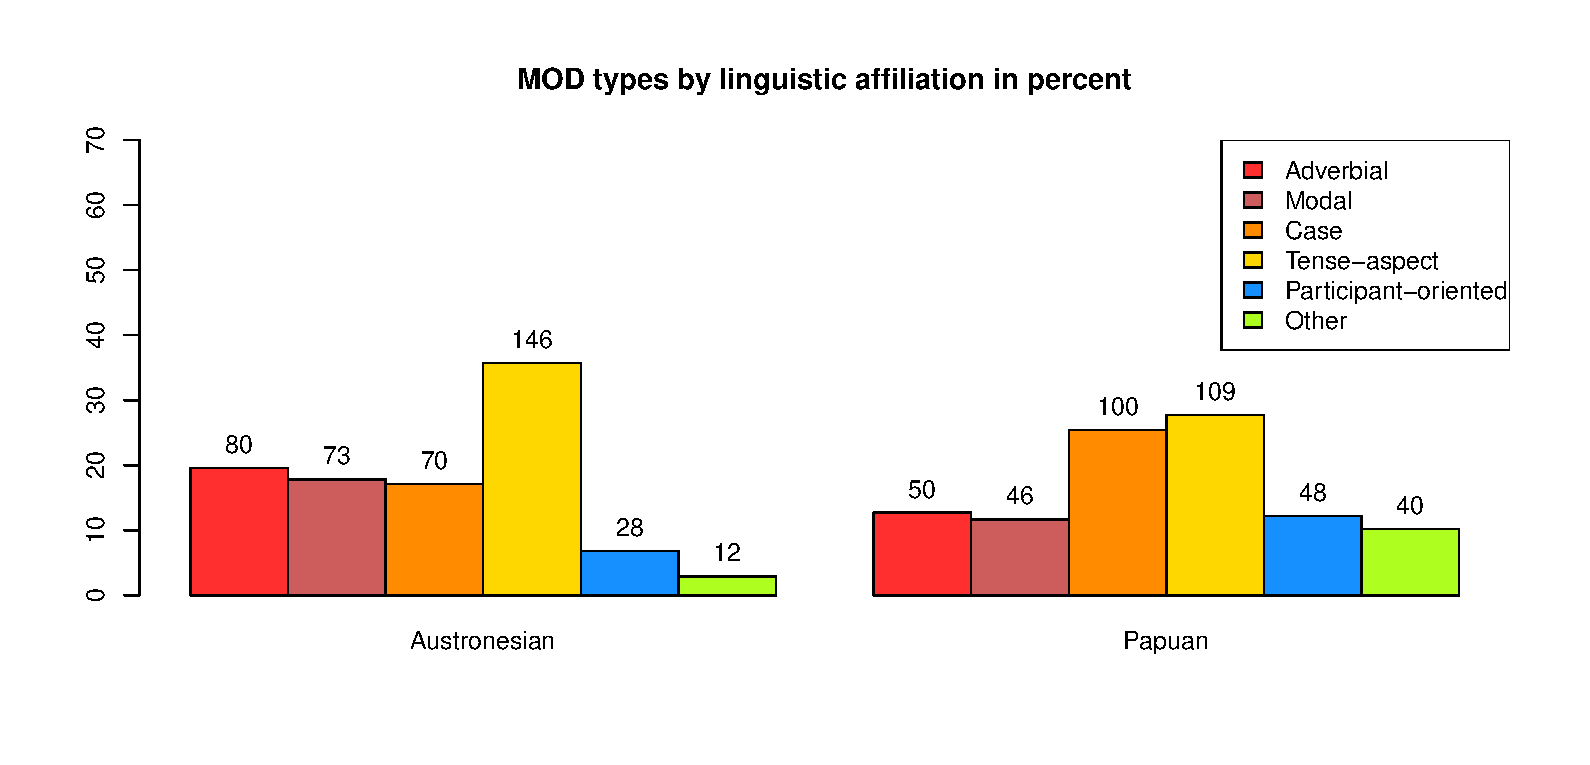
\includegraphics[width=\columnwidth]{figures/MOD_Family.eps}
\caption[MOD types by linguistic affiliation]{MOD types by linguistic affiliation. Numbers on top of the bars refer to the number of observations in the dataset.}\label{fig:mod-family}
\end{figure}
\begin{figure}
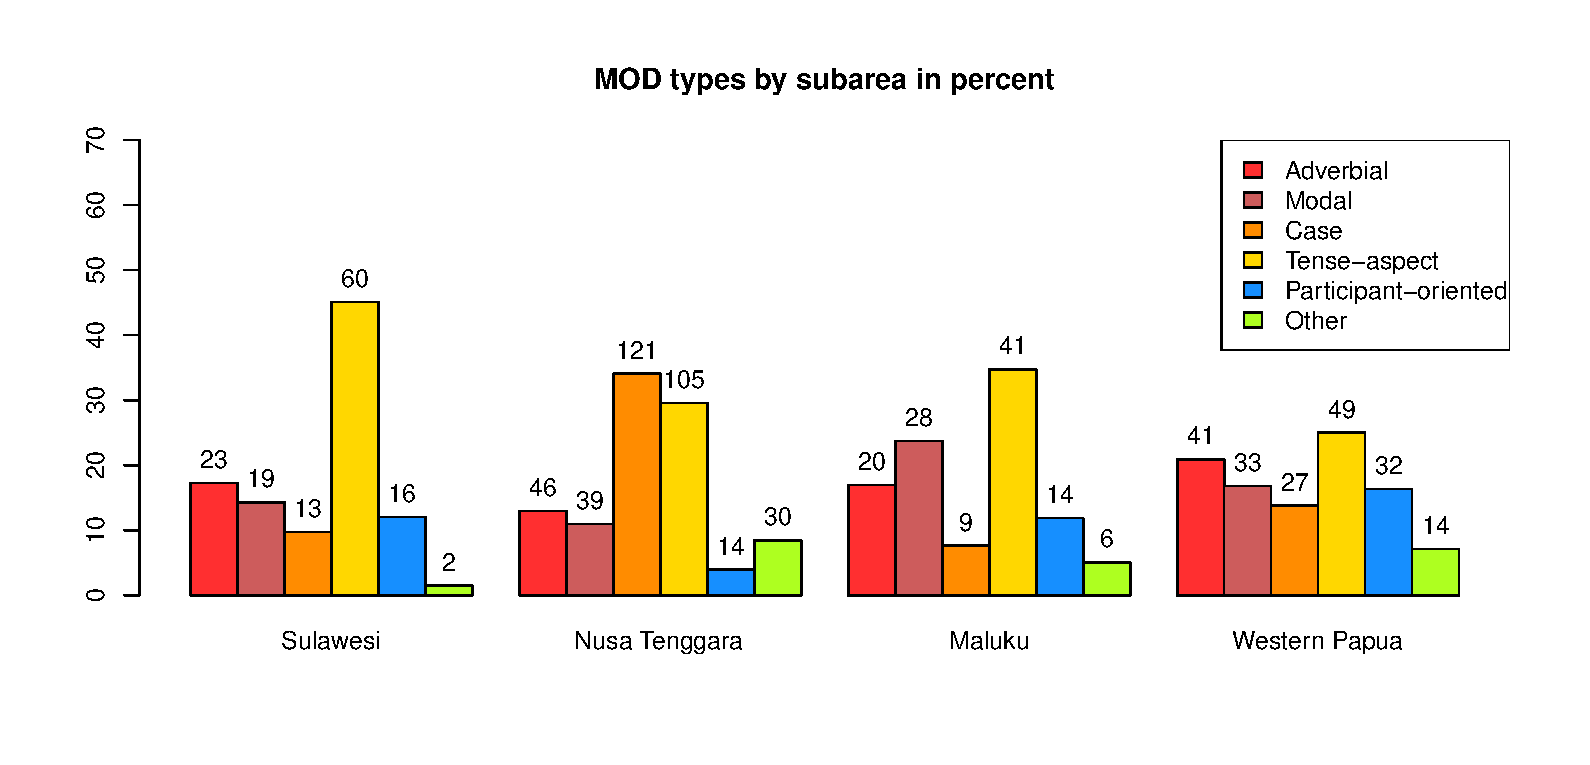
\includegraphics[width=\columnwidth]{figures/MOD_Group.eps}
\caption[MOD types by subarea]{MOD types by subarea. Numbers on top of the bars refer to the number of observations in the dataset.}\label{fig:mod-group}
\end{figure}


%Table \ref{table:MOD_language} below is a computation of \textsc{mod} construction numbers by language. As might be expected, a more fine-grained resolution of \textsc{mod} distribution across the dataset reveals further patterns. In the Sulawesi languages we again find the by now familiar division into northern Sulawesi languages (Pendau, Tajio), envisaging very little use of \textsc{mod} MVCs, and into the south-eastern languages for which \textsc{mod} use is clearly a pervasive phenomenon. Some other languages also deviate from the general picture by only using one of the functional groups, and in very small numbers. For Alorese (\textsc{nus} subarea) and Abun (\textsc{pap}) only adverbial constructions could be found. Dusner only contributes observations of case-marking constructions to the dataset. And finally, Sougb only has modal \textsc{mod} constructions, or so the numbers suggest.

%\begin{table}
%\begin{footnotesize}
%\begin{tabular}{lrrrrrr}
%  \lsptoprule
%  & \multicolumn{4}{c|}{event-oriented} & & \\
% & {adverbial} & {modal} & {case} & {tense-aspect|} & {participant-oriented} & {other}\\ 
%  \hline
%  Muna &   6 &   3 &   2 &  12 &   8 &   1 \\ 
%  Pendau &   0 &   1 &   0 &   3 &   1 &   0 \\ 
%  Tajio &   5 &   0 &   0 &   1 &   0 &   0 \\ 
%  Tolaki &   4 &   1 &   0 &  33 &   2 &   0 \\ 
%  TukangBesi &   8 &  14 &  11 &  11 &   5 &   1 %\\ \hline
%  Abui &   3 &  14 &  30 &  15 &   3 &   8 \\ 
%  Alorese &   4 &   0 &   0 &   0 &   0 &   0 \\ %
%  Bunaq &  15 &   1 &   0 &  28 &   3 &   8 \\ 
%  Kaera &   0 &   0 &   2 &   0 &   0 &   2 \\ 
%  Kambera &   1 &   2 &  18 &   3 &   0 &   0 \\ %
%  Klon &   6 &   8 &  16 &   9 &   0 &   1 \\ 
%  Makalero &   5 &   5 &  28 &   4 &   1 &   5 %\\ 
%  Teiwa &   5 &   0 &   3 &   9 &   0 &   0 \\ 
%  Tetun &   0 &   0 &  13 &  10 &   3 &   0 \\ 
%  Waimaqa &   5 &   9 &   8 &  24 &   0 &   6 \\ %
%  WesternPantar &   2 &   0 &   3 &   3 &   4 & %  0 \\ \hline
%  Buru &  12 &  11 &   0 &   9 &   1 &   0 \\ 
%  Selaru &   2 &   7 &   5 &   0 &   2 &   1 \\ 
%  Taba &   2 &   4 &   2 &  11 &   1 &   2 \\ 
%  Tidore &   4 &   4 &   2 &   8 &   2 &   3 \\ 
%  Tobelo &   0 &   2 &   0 &  13 &   8 &   0 \\ %\hline
%  Abun &   1 &   0 &   0 &   0 &   0 &   0 \\ 
%  Biak &   5 &   7 &   0 &   2 &   2 &   0 \\ 
%  Dusner &   0 &   0 &   9 &   0 &   0 &   0 \\ 
%  Hatam &   0 &   0 &   0 &   1 &   5 &   0 \\ 
%  Inanwatan &   0 &   0 &   0 &   1 &   0 &   3 %\\ 
%  Maybrat &   0 &   3 &  15 &   3 &   8 &   1 \\ %
%  Mor &   1 &   1 &   0 &   3 &   2 &   0 \\ 
%  Moskona &   8 &   1 &   0 &  13 &   7 &   9 \\ %
%  Mpur &   1 &   5 &   1 &   2 &   7 &   0 \\ 
%  Sougb &   0 &   3 &   0 &   0 &   0 &   0 \\ 
%  Wooi &  25 &  13 &   2 &  24 &   1 &   1 \\ 
%   \hline
%   \end{tabular}
%   \end{footnotesize}
%   \caption{Distribution of attested %\textsc{mod} constructions across languages}
%\label{table:MOD_language}
%\end{table}

Turning to the morphosyntactic properties of \textsc{mod} constructions, we find a much more diverse picture than with component-relating constructions in the previous section. This is hardly surprising as the latter form a small set of uniform constructions that seem to exhibit little variation across EI. Modifying constructions, on the other hand, are a heterogeneous pool of constructions with similar functions that are strongly influenced by the respective source lexemes of the modifier verb, as well as the specific grammaticalisation cline. This leads to the picture illustrated by Table \ref{table:mod_formal} below. The numbers show that the majority of \textsc{mod} MVCs still conforms to the default \textsc{MVC} that became visible at the end of Chapter \ref{ch:gram}: a construction with arguments tied together in `same subject' fashion, with inflection found on two verbs placed adjacent to each other. \textsc{mod} constructions as well are preferentially construed with the same subject pattern (the second most frequent argument configuration being event-to-argument reanalysis ``E"), a double-head marking is prevalent, and the verbs mostly appear in contiguous sequence. What is noticable, though, is that \textsc{mod} constructions do not exhibit the same amount of variation with respect to contiguity (the two most extreme values, ``3" and ``4" constituents intervening, are missing).

\begin{table}
\centering
\begin{tabular}{rrrrrrr}
  \lsptoprule
Referentiality & S & SO & D & A & E & X \\ 
  \hline
  adverbial &  74 &   2 &   6 &   0 &  48 &   0 \\ 
  modal &  95 &   0 &   0 &   1 &  16 &   7 \\ 
  case & 126 &   0 &  21 &   3 &  17 &   3 \\ 
  tense-aspect & 179 &   2 &   9 &   0 &  61 &   4 \\ 
  participant-oriented &  58 &   0 &  11 &   1 &   6 &   0 \\ 
  other &  27 &   0 &   4 &   0 &  20 &   1 \\ 
   \hline
 \\
  \hline
Headedness & B & 1 & 2 & S & N \\ 
  \hline
  adverbial &  35 &  18 &   0 &  13 &   6 \\ 
  modal &  57 &   2 &   8 &   3 &   1 \\ 
  case &  25 &  21 &   1 &  19 &   1 \\ 
  tense-aspect &  71 &  48 &   4 &   8 &  13 \\ 
  participant-oriented &  52 &   1 &   1 &   4 &   3 \\ 
  other &  11 &   6 &   3 &   1 &   1 \\ 
   \hline
 \\
  \hline
Contiguity & W & C & 1 & 2 \\ 
  \hline
  adverbial &   1 & 118 &  11 &   0 \\ 
  modal &   0 &  99 &  18 &   2 \\ 
  case &   0 & 127 &  43 &   0 \\ 
  tense-aspect &   4 & 220 &  27 &   4 \\ 
  participant-oriented &   0 &  58 &  16 &   2 \\ 
  other &   3 &  42 &   7 &   0 \\ 
   \lspbottomrule
\end{tabular}
\caption[Morphosyntactic properties of \textsc{mod} constructions]{Morphosyntactic properties of \textsc{mod} constructions in EI. Table components from top to bottom refer to referentiality (see §\ref{sec:argumentstructure}), headedness (see §\ref{sec:headedness}), and contiguity (see §\ref{sec:contiguity}), respectively.}
\label{table:mod_formal}
\end{table}

The following sections turn to the different functional groups introduced above, and provide examples from different constructions and subareas.

\subsection{Adverbial}\label{sec:adverbial}

Adverbial \textsc{mod} constructions cover two groups of modifier verbs that fulfill `adverbial functions'. Adverbial constructions proper contribute adverb-semantics that in non-serialising languages such as English are expressed by adjectives or adverbs. In this group of \textsc{mod} constructions, the modifying verb is recruited from a class of stative verbs. The second group, manner \textsc{mod}s, are made of what seem to be full-fledged verbs that are used in the modifier slot of the construction. As a heuristic, I assumed that such instances of \textsc{mod} constructions could be translated with the help of the phrase ``do X in Y manner", where X is the matrix verb, and Y refers to the semantics of the modifying verb. Table \ref{table:adverbial} presents the basic numbers. 

\begin{table}
\begin{tabular}{ll}
\lsptoprule
Feature&Value\tabularnewline
\hline
Template&V1 \textsc{matrix verb} * V2 \textsc{modifier verb}\tabularnewline
No. of attested instances& 130/2146 \tabularnewline
No. of attested languages& 23/32 \tabularnewline
Distribution across areas& \textsc{sul} (4/5), \textsc{nus} (9/11), \textsc{mal} (4/5) \textsc{pap} (6/11) \tabularnewline
Distribution across families& \textsc{pap} (10), \textsc{aus} (13) \tabularnewline
\lspbottomrule
\end{tabular}
\caption[Template and basic distribution of adverbial \textsc{mod} MVCs]{Template and basic distribution of adverbial \textsc{mod} MVCs in the EI sample. The asterisk indicates that matrix verb and modifier verb may occur in both positions.}
\label{table:adverbial}
\end{table}

The percentages from Figure \ref{fig:mod-group} above seem to indicate that adverbial modification is most widespread in the Western Papua languages. As Table \ref{table:MOD_language} shows, however, most instances come from just one language, the corpus language Wooi, and in fact only 6 of 11 \textsc{pap} languages display multi-verbal adverbial constructions. Wooi has two constructions of adverbial MVCs. First, there is a small class of stative verbs that are able to take inflection, and appear close to the matrix verb they modify. This pattern is illustrated in example (\ref{wooi_37}) with the modifier of speed, \textit{mararu}. The example consists of two MVCs, a motion complex formed by \textit{vavu} and \textit{taveri}, and a modifying constructions where \textit{mararu} is added. Note that both the component-relating process as well as the modification by \textit{mararu} do not add further spatiotemporal stages to the event scheme. The third verb, \textit{taveri}, remains uninflected due to its deranked status within the motion complex, but would in other contexts inflect as well. As \textit{mararu} seems to modify the whole motion complex, I assume that the modifying construction forms only after the motion verbs merge their components. However, the exact scope of the modifier verb remains ambiguous in many examples (alternatively one might assume here that \textit{mararu} targets the matrix verb \textit{vavu}, and the whole modified motion construal is then specified by \textit{taveri}).

\ea \label{wooi_37}
\langinfo{Wooi}{Austronesian, SHWNG}{HIVIAY\_exp}\\
\glll tamararu tambavu taveri \\
ta-mararu ta-vavu taveri \\
1\textsc{pl}.\textsc{in}-fast 1\textsc{pl}.\textsc{in}-return.home return \\
\glft `(And) we (can) go home fast.'\\ 
\z

A second adverbial MVC pattern involves postverbs that do not normally appear without a matrix verb. These are always construed with a shared set of verbal affixes (which is not always visible if there is no resumptive object suffix attached to the postverb, such as \textit{-a} below). Example (\ref{wooi_30}) is a typical case.

\ea \label{wooi_30}
\langinfo{Wooi}{Austronesian, SHWNG}{MANTERA\_magic\_charms}\\
\glll tatong harata mara \\
ta-ong hara=a mara \\
1\textsc{pl}.\textsc{in}-use wrong=\textsc{obj}.\textsc{nsg} \textsc{top} \\
\glft `If we use it wrongly...'\\ 
\z

A number of EI languages derives such modifiers by way of reduplication, and they are mostly considered adverbs, not verbs proper. This is why examples like the following one from Kaera have been excluded from the sample. Note, however, that in some languages `adverbial' modifiers are treated as verbs (by the respective authors) despite their reduplicated form, as in example (\ref{Bunaq17}) from Bunaq. The distribution of adverbial MVCs would thus be more widespread in EI if all instances of reduplicated modifiers were counted as verbs\footnote{Excluding all instances of reduplication in verbs would seem not helpful either as this would also pertain to dynamic verbs where reduplication in EI frequently produces Aktionsart differences, such as iterative or intensive readings.}.

\ea \label{}
\langinfo{Kaera}{Papuan, TAP}{\citealt[138]{klamer2014kaera}}\\
\gll ging kali~kali ekeng \\
3\textsc{pl} \textsc{rdp}~slow climb.up \\
\glft `They climb up slowly.'\\ 
\z

\ea \label{Bunaq17}
\langinfo{Bunaq}{Papuan, TAP}{\citealt[451]{schapper2009bunaq}}\\
\gll leleq enoq~enoq \\
flow slow~\textsc{rdp} \\
\glft `(The water) runs really slowly.'\\ 
\z

Manner constructions are formed by combining LLEs from two active verbs, most of them process verbs. The verbs that are in modifying function can also appear in simplex predicates elsewhere. Two major semantic fields may be distinguished. First, motion LLEs are modified by verbs denoting manner of motion, or otherwise compatible concepts that can be carried out during the motion process. Example (\ref{Bunaq_87}) from Bunaq illustrates such a case where the second verb provides information on the intention of the motion process (``in flight"). 

\ea \label{Bunaq_87}
\langinfo{Bunaq}{Papuan, TAP}{\citealt[472]{schapper2009bunaq}}\\
\gll Tebe tama sai, borus ciwal liol \\
return enter exit move.through flee continue \\
\glft `In turn (she) went in (then) out, continuing going through in flight.’\\ 
\z

Second, verbs of searching are quite often found in modifying function. The Biak case in (\ref{Biak_18}) shows such a construal, again together with a motion LLE, forming a motion PLE with manner specification. Verbs of searching are, however, also found accompanying non-motion verbs (for instance, \textsc{call} someone in a searching manner).

\ea \label{Biak_18}
\langinfo{Biak}{Austronesian, SHWNG}{\citealt[189]{vanheuvel2006}}\\
\glll Rofan anine ifrar syéwaro romámkun anine \\
rofan an-i-ne i-frar s$<$y$>$éwar=o romá-mkun an-i-ne \\
dog \textsc{giv}-3\textsc{sg}.\textsc{spec}-this 3\textsc{sg}-run $<$3\textsc{sg}$>$seek=O child-little \textsc{giv}-3\textsc{sg}.\textsc{spec}-this \\
\glft `This dog ran seeking for this child.'\\ 
\z

\subsection{Modal}\label{sec:modal}

Modal \textsc{mod} constructions convey a range of functions that are expressed in non-serialising languages by modal verbs, interrogative pronouns, permissives, evidential and hypothetical elements, among others. The functional common ground of all these is that the default factual mode of the utterance is modified, either in terms of agent-related properties (desiderative, abilitative, deontic),  with respect to event status (evidential, hypothetical, conative), or discourse-related (interrogative, hortative). The two latter functions are only rarely attested in the EI dataset for very few languages; the bulk of modal \textsc{mod} constructions refer to agent-related modification, that is desiderative, abilitative, and, to a lesser degree, deontic semantics. Table \ref{table:modal} summarizes the main facts about the distribution of \textsc{mod} constructions across EI, showing that the majority of EI languages utilise \textsc{mod} MVCs at least for some of the functions.

\begin{table}
\begin{tabular}{ll}
\lsptoprule
Feature&Value\tabularnewline
\hline
Template&V1 \textsc{matrix verb} * V2 \textsc{modifier verb}\tabularnewline
No. of attested instances& 119/2146 \tabularnewline
No. of attested languages& 22/32 \tabularnewline
Distribution across areas& \textsc{sul} (4/5), \textsc{nus} (6/11), \textsc{mal} (5/5) \textsc{pap} (7/11) \tabularnewline
Distribution across families& \textsc{pap} (11), \textsc{aus} (11) \tabularnewline
\lspbottomrule
\end{tabular}
\caption[Template and basic distribution of modal \textsc{mod} MVCs]{Template and basic distribution of modal \textsc{mod} MVCs in the EI sample. The asterisk indicates that matrix verb and modifier verb may occur in both positions.}
\label{table:modal}
\end{table}

Two main groups may be distinguished: (i) constructions with pseudo-modals that resemble modal verb constructions (but do not show the usual distinctions in finiteness), and (ii) adverb- or pronoun-like elements that morphosyntactically behave like verbs (or are treated as such by the respective data sources). The following examples illustrate typical constructions from the first group. The pair of examples in (\ref{Taba_29}) and (\ref{Taba_30}) from Taba exemplify what I take to be a core property of \textsc{mod} constructions, at least in prototypical cases: that the modifying constituent has gained the status of an independent constituent under the grammaticalisation process, and may occur in different positions within the clause (if the respective language does not require absolutely rigid constituent order in the clause). In the Taba example, neither the principle of iconic ordering nor any other rigid constructional template constrains the use of \textit{ahan}. Although this freedom of ordering does not exist in many other instances of \textsc{mod} constructions, it could be predicted that \textsc{mod} constructions in different languages grammaticalising similar lexemes display differential ordering of matrix verb and modifier verb (depending on the source lexeme, and its original position). This variation sets \textsc{mod} constructions apart from component-relating and stage-relating constructions, which are always guided by general ordering principles.

\ea \label{Taba_29}
\langinfo{Taba}{Austronesian, SHWNG}{\citealt[316]{bowden2001taba}}\\
\glll npe nahan \\
n=pe n=ahan \\
3\textsc{sg}=do 3\textsc{sg}=be.able \\
\glft `He can do it.'\\ 
\z

\ea \label{Taba_30}
\langinfo{Taba}{Austronesian, SHWNG}{\citealt[316]{bowden2001taba}}\\
\glll wwe nahan ncagal \\
wwe n=ahan n=sagal \\
leg 3\textsc{sg}=be.able 3\textsc{sg}=step \\
\glft `My leg would be able to walk.'\\ 
\z

The most frequent cases of pseudo-modals are desiderative constructions that express desire, want or intention of the actor to perfom the action contributed by the matrix verb. Here are two examples from different subareas. The first example in (\ref{Bunaq_2}) shows the only case in the dataset where the desiderative verb comes second and not first (despite the fact that Bunaq is an AVO language). Recall from §\ref{sec:criteria_mvcs} that modifying constructions do not show constant behaviour in terms of operator placement. While TAM and person indexing operator values are typically shared across all verbal constituents in \textsc{mod} constructions, this is not true for negation, where at least in some \textsc{mod} constructions, negation of just one constituent seems possible. The Bunaq example in (\ref{Bunaq_2}) reflects this behaviour as the prospective marker \textit{gie} here only targets the motion constituent. This is in contrast to component-relating and stage-relating constructions in Bunaq where operators such as \textit{gie} need to have scope over the entire construction (cf. \citealt[443f.]{schapper2009bunaq}).

\ea \label{Bunaq_2}
\langinfo{Bunaq}{Austronesian, TAP}{\citealt[444]{schapper2009bunaq}}\\
\gll baqi o mal gie heten \\
\textsc{nprx}.\textsc{an} \textsc{foc}.\textsc{add} go \textsc{prosp} want \\
\glft `She also wants to walk.’\\ 
\z

Example (\ref{Wooi111}) from Wooi illustrates the order desiderative verb -- matrix verb. At least in Wooi, this order reflects  original source properties of the modifier verb. The origin of \textit{o} `want' is still transparent in Wooi: it is derived from \textit{oyo} `say' which is also frequently attested in a short form \textit{o} (\textit{o} `want', however, is always short, and never appears as \textit{oyo}). Thus desiderative constructions with \textit{o} originated from speech complement constructions where the sentential complement followed the \textsc{say} verb (and eventually got reanalysed as matrix verb constituent of a desiderative construction).

\ea \label{Wooi111}
\langinfo{Wooi}{Austronesian, SHWNG}{HIVIAY\_exp}\\
\glll co vio to Nunoing vane \\
ti-o $<$i$>$vo to N. vane \\
3\textsc{sg}-want $<$3\textsc{sg}$>$row \textsc{dir} N. \textsc{det}.\textsc{nprx} \\
\glft `(For example, if) he wants to go to Miosnum...'\\ 
\z

Speech act complementation can have a shift in subject arguments (for instance, in \textit{I say you do} type constructions). Given that speech act complementation is the source of at least some of the desiderative MVCs coded here as \textsc{mod}s, this raises the question whether desideratives of this sort can have the same shift in arguments. In English, want constructions are overtly biclausal, and involve raising of the dependent clause subject to the object of the matrix clause in case the `wisher' is not co-referential with the referent that is supposed to perform the action. Think of something like \textit{I want Jones to butter his toast at midnight} where, in structural terms, Jones belongs to the subordinate clause but is raised to object status. Such constructions are also possible in some EI languages with the only difference that there is no cue as to a biclausal construal. Consider an example from Selaru.

\ea \label{Selaru_4}
\langinfo{Selaru}{Austronesian, CMP}{\citealt[112]{coward2005}}\\
\gll Majelis-ke r-buma ta-wahuk nur-Vre rahean.rahean \\
elders-\textsc{art} 3\textsc{pl}-want 1\textsc{pl}.\textsc{in}-gather coconut-\textsc{pl} ten.by.ten \\
\glft `The church elders want us to gather coconuts in tens.‘\\ 
\z

In Selaru both same-subject desiderative constructions, as well as ones without argument sharing, as in (\ref{Selaru_4}), are equally licit. Argument interaction in such examples has been coded ``X" as the exact argument relation between the constituents is not made transparent by morphosyntactic marking (note that such examples explain the conspicuous number of 7 ``X" cases for modal \textsc{mod} constructions in Table \ref{table:mod_formal} above). This is, however, not the case in all languages. Wooi is different in this regard. We might expect to find a conceptual overlap between speech act complements (I say he takes), and desiderative readings (I want him to take), but this is not supported by the Wooi data corpus. Each time there is a shift in subject indexing between \textsc{say}/\textsc{want} and matrix verb, the translation given indicates that the construction is still understood in its literal sense as a speech complement.\footnote{Note that the interrelatedness between cognitive verbs like \textsc{wish}, and speech verbs like \textsc{say} reflects the deeper cultural doctrine of the `opacity of other minds' that is well-developed in many languages from New Guinea and parts of Oceania. Opacity of the other mind describes what can be perceived as a cultural reluctance of stating directly what other people think or believe, as this is deemed impossible to know from an outside perspective. Instead of saying, for instance, \textit{Jones wants to eat toast at midnight}, one would rather resort to a behaviorist interpretation \citep{robbins2008not} like \textit{Jones says he eats toast at midnight}, thus circumventing a direct statement about Jones' inner feelings. See \citet{robbins2008introduction, robbins2008not, rumsey2013intersubjectivity} on the opacity of other minds.}

Turning to the second group of modal \textsc{mod} constructions, we find adverb or pronoun-like elements that take inflection and behave like a full-fledged verb. These \textsc{mod}s are rare in the dataset and basically confined to south-eastern Sulawesi and some odd examples from Papuan languages of the TAP area (Abui, Makalero). The following examples from Tukang Besi show an interrogative pronoun that is inflected like a verb in (\ref{Tukang_17}), and an evidential construction in (\ref{Tukang_18}). Comparable constructions are otherwise hardly found in the dataset.

\ea \label{Tukang_17}
\langinfo{Tukang Besi}{Austronesian, WMP}{\citealt[191]{donohue1999}}\\
\gll o-ha'a tabeda to-wila loeloe? \\
3\textsc{rls}-why necessary 1\textsc{pl}.\textsc{rls}-go slowly \\
\glft `Why will we have to go slowly?'\\ 
\z

\ea \label{Tukang_18}
\langinfo{Tukang Besi}{Austronesian, WMP}{\citealt[189]{donohue1999}}\\
\gll o-tantu no-rato sabentara \\
3\textsc{rls}-certain 3\textsc{rls}-arrive in.a.moment \\
\glft `They'll be here in a moment for certain.' (i.e., 'It is certain they will arrive in a moment')\\ 
\z

\subsection{Case-marking} \label{sec:case-marking}

Case-marking is here understood in a non-strict sense: case-marking \textsc{mod} constructions comprise all those cases in which a (transitive) modifier verb introduces a further argument to the argument frame of the construction. This argument typically belongs to a set of oblique (adjunct) arguments, but some constructions seem to introduce core arguments as well. Attested arguments are direct object (patient, theme), experiencer, recipient, benefactive, comitative, instrumental, locative, source, and goal. Such MVCs have been identified in many serialising languages and can be considered one major group of prototypical SVCs according to many analyses (for instance \citealt{givon1991serial, Aikhenvald2006, haspelmath2016serial}; see also \citealt{lord1993historical} on the diachronic development of case-marking constructions in African languages). Table \ref{table:case} illustrates the basic facts on the distribution of case-marking MVCs across the EI area.

\begin{table}
\begin{tabular}{ll}
\lsptoprule
Feature&Value\tabularnewline
\hline
Template&V1 \textsc{matrix verb} * V2 \textsc{modifier verb}\tabularnewline
No. of attested instances& 170/2146 \tabularnewline
No. of attested languages& 18/32 \tabularnewline
Distribution across areas& \textsc{sul} (2/5), \textsc{nus} (9/11), \textsc{mal} (3/5) \textsc{pap} (4/11) \tabularnewline
Distribution across families& \textsc{pap} (9), \textsc{aus} (9) \tabularnewline
\lspbottomrule
\end{tabular}
\caption[Template and basic distribution of case-marking \textsc{mod} MVCs]{Template and basic distribution of case-marking \textsc{mod} MVCs in the EI sample. The asterisk indicates that matrix verb and modifier verb may occur in both positions.}
\label{table:case}
\end{table}

As I have already noted above, case-marking MVCs can be considered a special feature of the Nusa Tenggara subarea as 121 from 170 instances are from \textsc{nus} languages. Nine of 11 Nusa Tenggara languages have such constructions, with Abui and Makalero being particularily productive in this regard.

Introduction of direct object arguments is only found in Makalero. The \textsc{take} verb \textit{mei} has developed into a light verb introducing arguments in case the main verb's object slot is already taken, for instance by a member of the large complement class \citep[203f.]{huber2011}. Verbal argument frames in Makalero may not exceed the number of two arguments. Therefore, when the object slot is in use, the addition of another argument slot is brought about by employing \textit{mei}. Examples (\ref{Makalero_56}), (\ref{Makalero_61}) and (\ref{Makalero_18}) illustrate three instances where the lightverb \textit{mei} is used. Each one adds a different kind of argument to the argument frame of the construction, making \textit{mei} a valency increaser with a broad range of functional context. In example (\ref{Makalero_56}), \textit{mei} introduces the object-theme \textit{Timor} because the ``complement-verb complex" (see \citealt[131f.]{huber2011}) consisting of matrix verb \textit{kini/ini} `do' and its complement \textit{lafu'} already constitute a saturated transitive argument frame. Note that Makalero has two kinds of linkers, \textit{=ini} and \textit{=isi}, both of which Huber analyses as clause linkers \citep[457f.]{huber2011}. Given, however, that at least \textit{=ini/ni} often appears in positions that obviously connect verbs of tightly bound constructions, I am assuming here that \textit{=ini/ni} rather provides a means to overtly extablish an integral construction rather than marking off two different clauses. Its use appears to be optional rather than required by the lightverb, as examples (\ref{Makalero_61}) and (\ref{Makalero_18}) are grammatical without a linker.

\ea \label{Makalero_56}
\langinfo{Makalero}{Papuan, TAP}{\citealt[169]{huber2011}}\\
\gll negara taure’=ini tone’ ma’u=ni Timor ere mei=ni lafu’-ini \\
nation which=\textsc{ctr} perhaps come=\textsc{lnk} T. 1\textsc{dem} take=\textsc{lnk} live-do:\textsc{bd} \\
\glft '...whichever nation comes and rescues Timor...’\\ 
\z

The next example in (\ref{Makalero_61}) shows the introduction of another theme-object. According to Huber's analysis, the object argument added by \textit{mei} is read as an instrument \citep[204]{huber2011}. This is indeed the case, but only at the level of the construction. It is the context rather than \textit{mei} by itself that invokes the instrument reading of the referent.

\ea \label{Makalero_61}
\langinfo{Makalero}{Papuan, TAP}{\citealt[204]{huber2011}}\\
\gll Nana-uai aire’ sa’a-mei tina-ini? \\
elder.sibling-\textsc{hon} now what:\textsc{bd}-take cook-do:\textsc{bd} \\
\glft ‘With what are you cooking?’\\ 
\z

Another use of \textit{mei} is in complex argument frames pertaining to construals of perception. In example (\ref{Makalero_18}) \textit{fi lolo-ini ere}, our language, is the stimulus of the perception event. It is first introduced by transitive \textit{mei}, and then, as I understand it, reintroduced as subject argument of an intransitive \textit{puna} `look'. So, literally, I would expect something along the lines of `our language, we take (it), it looks very bad'.

\ea \label{Makalero_18}
\langinfo{Makalero}{Papuan, TAP}{\citealt[189]{huber2011}}\\
\gll po fi lolo-ini ere fi=haka e’=ini mei puna hanu pa’u$~$pa’uk \\
\textsc{adv} 1\textsc{pl}.\textsc{in} say-\textsc{nm} 1\textsc{dem} 1\textsc{pl}.\textsc{in}=\textsc{ctrpres} \textsc{dem}=\textsc{lnk} take look very \textsc{rdp}$~$bad \\
\glft ‘But our language, we see it as very bad...’\\ 
\z

Up to this point, the other EI languages have not contributed any examples. They only enter the picture when we turn to the introduction of adjunct arguments. Here we may distinguish two groups: (i) circumstantial arguments involve benefactives, comitatives and instruments; (ii) and local arguments comprise source, locative and goal arguments. Benefactive MVCs occur in four languages, Tukang Besi from the Sulawesi group, Makalero and Abui from Nusa Tenggara, and the language isolate Maybrat from the Bird's Head (Western Papua). I have already illustrated benefactive MVCs from these languages in §\ref{sec:modification} on the semantics of modification.

Comitative and instrument constructions are more common throughout EI, but it is still only a minority of languages that have attested examples. Both groups of constructions may use a modifier verb that is glossed as 'with' (among other verbs that are specific to either constructional group, such as \textsc{accompany} verbs in comitative constructions). Maybrat even employs two different \textsc{with} verbs, one for each construction. Comitatives are attested for Tukang Besi, Abui, Western Pantar, Tetun Fehan, Waima'a, Teiwa, Selaru and Maybrat. The following pair of examples from Tetun again shows that at least some of the modifying MVCs allow the modifier consituent to be placed either before or after the matrix verb. At first glance the pattern seems identical as \textit{hó} `accompany' follows the directed motion verb \textit{bá} in each case. In example (\ref{Tetun_54}), however, the modifier verb is postponed after the matrix verb, while example (\ref{Tetun_57}) shows what I take to be a case of stacked MVCs: the modifying construction is nested into the action slot of a matrix motion-to-action MVC. Thus, the order \textit{bá} \textit{hó} looks just the same in both examples, but the directed motion verb in example (\ref{Tetun_57}) is in fact not part of the modifying construction. That is, in example (\ref{Tetun_57}) the modifier verb is preposed to its matrix verb \textit{k-adiuk}. This analysis is supported by van Klinken's own analysis (cf. \citealt[272]{vanklinken1999grammar}): the comitative relation only holds true at the time of the playing, but not at the precursor motion phase.

\ea \label{Tetun_54}
\langinfo{Tetun Fehan}{Austronesian, CMP}{\citealt[272]{vanklinken1999grammar}}\\
\gll ha'u bá k-ó lós Am Bo'uk dei \\
1\textsc{sg} go 1\textsc{sg}-accompany just father Bo'uk only \\
\glft `I will go with only Am Bo'uk. (i.e. No-one else will go)'\\ 
\z

\ea \label{Tetun_57}
\langinfo{Tetun Fehan}{Austronesian, CMP}{\citealt[272]{vanklinken1999grammar}}\\
\gll ha k-bá k-ó feto sia k-adiuk \\
1\textsc{sg} 1\textsc{sg}-go 1\textsc{sg}-accompany woman \textsc{pl} 1\textsc{sg}-play \\
\glft `[Every evening,] I go and play with (i.e. court) the girls.'\\ 
\z

Note that \textit{hó} still appears to maintain a more concrete lexical meaning than, say, a verb that is only glossed as `with'. The next example is from Selaru, and shows such a case with a stripped-down comitative verb. Note again that comitative verbs may come either before or after the matrix verb, at least from a crosslinguistic perspective. This is in sharp contrast to what we find with both component-relating and stage-relating constructions.

\ea \label{}
\langinfo{Selaru}{Austronesian, CMP}{\citealt[120]{coward2005}}\\
\gll Y-aso sir ma r-al-a kotw ti enen desike y-or amam desike ra ma ktei \\
3\textsc{sg}-request them \textsc{conj} 3\textsc{pl}-give-Ø food \textsc{conj} woman that(\textsc{art}) 3\textsc{sg}-with man that(\textsc{art}) they.eat until done \\
\glft `He requested they give the food so that woman and that man [can] eat until done...'\\ 
\z

Instrumental MVCs are attested for Kambera, Klon, Tetun Fehan, Taba, Tidore, and Maybrat. In Kambera, instrumental MVCs are construed with a \textsc{use} verb, \textit{wàngu}. Here are three examples. In (\ref{Kambera_22a}), \textit{wàngu} is placed after the matrix verb, and this is the default position. In case the \textit{wàngu} VP is topicalised, it can precede the matrix verb, however, by changing its syntactic status through the use of a linker \textit{ba}, as example (\ref{Kambera_22b}) shows. Another possible manipulation of (\ref{Kambera_22a}) is focusing of the instrument argument licensed by \textit{wàngu}. Preposing \textit{huru}, the spoon, in example (\ref{Kambera_22c}) leaves the orginal order with a postposed \textit{wàngu} intact. One could argue that the Kambera case with \textit{wàngu} is just the same as the Makalero lightverb \textit{mei} in that both modifier verbs license a direct object argument. The reason for placing \textit{mei} in the direct object group above, and \textit{wàngu} in the instrumental argument group is that the former must have (at least originally) taken a theme object, while a \textsc{use} verb could arguably pass instrument semantics on to its object argument\footnote{Kambera \textit{wàngu} is in fact one of those generic verbs that are hard to pin down semantically. It may in simplex predicate contexts have the meaning `use', `do', `say' (and, derived from say, `want'; \citealt[284ff.]{klamer1998grammar}). Therefore, placing the \textit{wàngu} construction in the group of instrumental MVCs heavily relies on the gloss `use'.}.

\ea 
\langinfo{Kambera}{Austronesian, CMP}{\citealt[287]{klamer1998grammar}}\\
\ea \label{Kambera_22a}
\gll ku-taku uhu wàngu huru \\
1\textsc{sg}.\textsc{nom}-scoop rice use spoon \\
\glft `I scoop rice with a spoon.' \\ 
\ex \label{Kambera_22b}
\gll wàngu huru ba ku-taku uhu \\
use spoon \textsc{conj} 1\textsc{sg}.\textsc{nom}-scoop rice \\
\glft `With a spoon I scoop rice.' \\ 
\ex \label{Kambera_22c}
\gll huru ku-taku uhu wàngu \\ 
spoon 1\textsc{sg}.\textsc{nom}-scoop rice use \\
\glft `I scoop rice with a SPOON.'\\ 
\z
\z

The group of local case-marking construction, namely source, locative, and goal, is better attested than the other case-marking constructions. They are mainly formed by the use of a locative verb (mostly glossed as `be', `be.in', `be.at'). What is interesting is that the position of the locative verb often indicates its function by obeying the iconicity of order. That is, a preposed locative verb marks source arguments, a postposed locative verb may mark a goal (see also \citealt{schapper2011iconicity} on source and goal encoding in Kamang and Bunaq). In Papuan head-final languages, however, the goal argument (with the locative verb) is usually placed before the matrix verb, indicating the somewhat grammaticalised nature of the modifier VP.

The first pair of examples in (\ref{Maybrat_60}) is from Maybrat, and illustrates a MVC introducing a source argument. Here, again, the order of both verbs seems interchangeable. Example (\ref{Abui_24}) is a source-marking construction from Abui. Locative verbs such as \textit{mi} are widespread across the TAP languages, and can express a range of different concepts, most of which are related to spatial semantics. When Abui \textit{mi} is construed with a motion verb, it marks the source or starting point of the motion process. Similar constructions can also be noticed in neighbouring languages, but sometimes a source NP is in fact lacking where it might be expected. Example (\ref{Klon_48}) illustrates such a case from Klon. It might be interpreted as covert source-marking: \textit{mi} adds a spatial starting point to the process of getting up, although no explicit mention is made of its exact location in the discourse space.

\ea \label{Maybrat_60}
\langinfo{Maybrat}{Papuan, isolate}{\citealt[206]{dol2007grammar}}\\
\ea
\gll t-ama t-pat Sorong \\
1\textsc{sg}-come 1\textsc{sg}-from S. \\
\glft `I come from Sorong.' \\ 
\ex
\gll ait y-pat rapuoh y-ama \\ 
3\textsc{m} 3\textsc{m}-from forest 3\textsc{m}-come \\
\glft `He comes from the forest.'\\ 
\z
\z

\ea \label{Abui_24}
\langinfo{Abui}{Papuan, TAP}{\citealt[356]{kratochvil2007grammar}}\\
\gll fala mi-a yaa! \\
house be.in-\textsc{dur} go \\
\glft `Go from the house!', lit. 'Be in the house, go!’\\
\z

\ea \label{Klon_48}
\langinfo{Klon}{Papuan, TAP}{\citealt[137]{baird2008grammar}}\\
\gll nang bo adob lega mi ihih \\
\textsc{neg} \textsc{seq} true 3\textsc{sg}.\textsc{top} be.at get.up \\
\glft `So he indeed got up.'\\ 
\z

In Klon, modifier VPs with \textit{mi} can also occur postverbally, where they typically mark the endpoint or goal of a motion event. In example (\ref{Klon_99a}) below, we see that \textit{mi} may introduce local case NPs. Note that the NP \textit{alah} `house' is governed by \textit{mi}, and not by \textit{qad} `come'. The next example from Klon in (\ref{Klon_99b}) illustrates that the case interpretation of the NP licensed by \textit{mi} depends on the semantics of the matrix verb. The first instance is quite naturally interpreted as the endpoint of ego returning to the place called Hwak. The second \textit{mi}, however, combines with a stative verb and specifies the location of the sleeping.

\ea \label{Klon_99a}
\langinfo{Klon}{Papuan, TAP}{\citealt[137]{baird2008grammar}}\\
\gll kuur angkol a~awar qad alah mi ik \\
dog self \textsc{rdp}~return come house be.at \textsc{compl} \\
\glft `The dog itself came back and was at home.'\\ 
\z

\ea \label{Klon_99b}
\langinfo{Klon}{Papuan, TAP}{\citealt[148]{baird2008grammar}}\\
\gll na lam gen u-elel, eben buur u-elel, Hwak mi awar, Hwak weer mi taa' \\
1\textsc{sg}.\textsc{act} walk until \textsc{vi}-search village flat \textsc{vi}-search Hwak be.at return Hwak river be.at sleep \\
\glft `I walked until I found, found a flat village and returned to Hwak, slept at Hwak river.'\\ 
\z

\subsection{Tense-Aspect}

The largest group of \textsc{mod} MVCs is formed by constructions that convey tense-aspect semantics (again understood here in a non-strict sense including Aktionsart concepts and all sorts of other temporal formatives), subsuming a wide range of different concepts. As in the modal group above, there are two sets of items that participate in such \textsc{mod} constructions. First, there is a large group of aspectual verbs that have been grammaticalised to different extents. And second, there is a much smaller group of adverb-like elements that behave like verbs and denote temporal concepts. The latter group is again more or less confined to the languages of south-eastern Sulawesi (Tolaki, Muna and Tukang Besi). Table \ref{table:tense-aspect} below presents the basic numbers of tense-aspect \textsc{mod} MVCs.

\begin{table}
\begin{tabular}{ll}
\lsptoprule
Feature&Value\tabularnewline
\hline
Template&V1 \textsc{matrix verb} * V2 \textsc{modifier verb}\tabularnewline
No. of attested instances& 255/2146 \tabularnewline
No. of attested languages& 26/32 \tabularnewline
Distribution across areas& \textsc{sul} (5/5), \textsc{nus} (9/11), \textsc{mal} (4/5) \textsc{pap} (8/11) \tabularnewline
Distribution across families& \textsc{pap} (13), \textsc{aus} (13) \tabularnewline
\lspbottomrule
\end{tabular}
\caption[Template and basic distribution of tense-aspect \textsc{mod} MVCs]{Template and basic distribution of tense-aspect \textsc{mod} MVCs in the EI sample. The asterisk indicates that matrix verb and modifier verb may occur in both positions.}
\label{table:tense-aspect}
\end{table}

The group of aspectual verbs is dominated by \textsc{begin}, \textsc{finish} and \textsc{complete} verbs. I coded constructions that focus on modifying the telicity of event construals (that is, denoting their beginning or ending) as aspectual proper, and distinguished another group of constructions (basically also involving verbs of finishing) that show signs of grammaticalisation towards completive semantics (that is, denoting actions affecting the totality of participants; see also \citealt{huber2014} on data from Bunaq, Kamang, and Makalero). Iconicity seems to be a factor in the formation of such MVCs as \textsc{begin} verbs normally precede the matrix verb, and \textsc{finish} verbs follow it. The following examples give an illustration of how such aspectual \textsc{mod} constructions look like in EI. Example (\ref{Tolaki_38}) is from Tolaki, and makes use of the inflection pattern typical for that language: only the first verb takes inflection, which is in this case the modifier verb (this order is, as I mentioned above, an exception among the EI  languages, as \textsc{finish} verbs typically come last). The next example in (\ref{Western_14}) is from Western Pantar, and illustrates two intertwined MVCs. The dying is construed as the direct result of the slicing by means of a stage-relating MVC. To this bi-stage event schema, an aspectual \textsc{mod} MVC is added, reinforcing the endpoint of the dying. \textit{Gaata} here might either be interpreted as modifying \textit{hinna} alone, that is, the second event stage, or it might be read as modifying the whole event schema, that is, both stages. As the latter interpretation would clash with the conceptual event hierarchies, as proposed in chapter \ref{ch:sem}, I assume that in such cases, only the event stage adjacent to the modifier verb is modified (yielding something like slice -- [die finish]) (but see also §\ref{sec:clauselevelmodification}).

\ea \label{Tolaki_38}
\langinfo{Tolaki}{Austronesian, WMP}{\citealt[123]{mead2008verb}}\\
\gll ari 'aku-to \\
finish-1\textsc{sg}.\textsc{abs} $<$M$>$:\textsc{antip}-eat \\
\glft `I've already eaten.'\\ 
\z

\ea \label{Western_14}
\langinfo{Western Pantar}{Papuan, TAP}{\citealt[82]{holton2014western}}\\
\gll a-ule pai hinna kanna gaata \\
4\textsc{sg} slice die finish already \\
\glft `They sliced his neck and killed him.'\\ 
\z

Example (\ref{Buru_35}) from Buru illustrates the case of aspectual MVCs with a \textsc{begin} verb. In Buru and elsewhere, \textsc{begin} verbs precede their matrix verb, but the position of the pronominal subject is less rigid, and may shift to a position between the two verbs (see \citealt[215]{grimes1991buru}). The following example from Moskona exemplifies the use of a non-prototypical modifier verb. I have at several points made mention of motion verbs attaining aspectual semantics. In Moskona, it is obvious that \textit{eyja} still retains part of its motion semantics, but it may also be read as highlighting the beginning of an event. This relation between a stage-relating interpretation (go-build), and a modifying one (begin-build) sheds light on the diachronic pathways that exist between the different techniques of MVC formation. As constructions acquire new readings they may also acquire a different interpretation of their underlying event construal (for instance, by shifting from a bi-stage event schema to a mono-stage one).

\ea \label{Buru_35}
\langinfo{Buru}{Austronesian, CMP}{\citealt[215]{grimes1991buru}}\\
\gll ringe peltanek iko boli fena-fena \\
3\textsc{sg} begin go perimeter \textsc{rdp}-village \\
\glft `He began to go around to each of the villages.'\\ 
\z

\ea \label{Moskona_48}
\langinfo{Moskona}{Papuan, EBH}{\citealt[297]{gravelle2010grammar}}\\
\gll edá, eri i-eyja i-or mod jig merga or-i-em tas \\
then they.\textsc{pl} 3\textsc{pl}-go 3\textsc{pl}-build house \textsc{loc} wood \textsc{num}:7-?-\textsc{contr} again \\
\glft `Then, they began again to build a house in another tree.’ \\
or `they went again [and] built a house in another tree.’\\ 
\z

Completives differ from \textsc{finish} semantics in that the endpoint of the event is not reached by some actor willfully ending it, but because a totality of referents is affected (see e.g. \citealt{bybee1994evolution} for a diachronic assessment of completives). Not all EI authors distinguish between completives and \textsc{finish} semantics. The difference, however, stands out clearly when the glossing or translation of \textsc{finish} verbs involves some meaning of `all', as for instance in Waima'a \textit{maa}, or in the  \textit{kay} construction from Wooi. Waima'a \textit{maa} is most often translated as `finish', but in some contexts the the translation and the glossing provided by the language consultant are markedly different, such as in example (\ref{wmh_x}) below. Here, \textit{maa} is glossed as `empty', indicating that the process of picking has ended because all the fruits had been picked. The completive semantics of \textit{maa} are also visible in examples such as (\ref{wmh_y}) where a wedding party prepares different kinds of items for the ceremony, and brings these items to the wedding place. \textit{Maa} in this context clearly does not refer to the endpoint of the bringing, but specifies the object of the bringing to include all items mentioned in the previous utterances. Completive MVCs such as these have been recorded in the EI sample for a couple of languages in the Nusa Tenggara, Maluku, and Western Papua groups, but not for any of the Sulawesi languages.

\ea \label{wmh_x}
\langinfo{Waima'a}{Austronesian, CMP}{pear\_Santina 025}\\
\gll ne la kai oo ta ne uhu ma'a ulo \\
3\textsc{sg} \textsc{loc} wood above \textsc{dist} 3\textsc{sg} pick empty already \\
\glft `After the one at the top of the tree is done with picking (fruit).'\\ 
\z

\ea \label{wmh_y}
\langinfo{Waima'a}{Austronesian, CMP}{dom2\_kaben 138}\\
\gll sire ani ma'a  ruo \\
3\textsc{pl} bring all with \\
\glft `They bring it all.'\\ 
\z

What is found in the south-eastern Sulawesi area and its vicinity instead is tense-aspect MVCs of the second group introduced above, namely MVCs that are formed by stative non-prototypical verbs. Instances of these group cluster in their constructional make-up with modal \textsc{mod}s as already discussed in §\ref{sec:modal} above. Here are three examples, each illustrating habitual modification by using a \textsc{mod} MVC. Although the languages use different head-marking strategies (first verb inflected in Tolaki versus all verbs inflected in same subject-manner in Muna and Tukang Besi), the overall constructional make-up is rather similar: the modifier verb comes first and is immediately followed by the matrix verb(s). Both Muna and Tukang Besi show what \citet{vandenberg1989} referred to as ``subject harmonisation", that is, the modifier verb takes the same subject indexer as the matrix verb(s). As the example from Muna in (\ref{Muna_30}) further illustrates, more than one modifier verb may combine with a single matrix verb.

\ea \label{Tolaki_39}
\langinfo{Tolaki}{Austronesian, WMP}{\citealt[123]{mead2008verb}}\\
\gll a-no ndee modea-'iro mbe-maroa i aahua-no\\
and-3\textsc{sg}.\textsc{nom} habitually $<$M$>$:hear-3\textsc{pl}.\textsc{abs} \textsc{coll}-be.noisy at well-3\textsc{sg}.\textsc{gen}\\
\glft '...and he usually heard them all being noisy at his well.'\\
\z

\ea \label{Tukang_62}
\langinfo{Tukang Besi}{Austronesian, WMP}{\citealt[510]{donohue1999}}\\
\gll te Wanse, o-monea na-po-daga na-para-aso, no-karajaa, a mo'ane, wowine \\
\textsc{core} Wanci 3\textsc{rls}-usual 3\textsc{irr}-\textsc{recp}-trade 3\textsc{rls}-\textsc{iter}-sell 3\textsc{rls}-work \textsc{nom} man woman \\
\glft `On Wanci, normally both men and women trade, and sell things, and work.' \\ 
\z

\ea \label{Muna_30}
\langinfo{Muna}{Austronesian, WMP}{\citealt[238]{vandenberg1989}}\\
\gll ao-nea ae-rimba a-kala \\
1\textsc{sg}.\textsc{rls}-usual 1\textsc{sg}.\textsc{rls}-fast 1\textsc{sg}.\textsc{rls}-go \\
\glft `Usually I walk fast.'\\ 
\z

\subsection{Participant-oriented}

The last four sections have dealt with modifying MVCs that target the event schema of a matrix verb, and add specific semantic content to it. I now turn to another group of \textsc{mod} MVCs that do not directly modify the event, but one of the participants that are associated with it. Participant-oriented MVCs are less frequent in the EI dataset, with 76 cases attested. Table \ref{table:participant} shows that only few instances are found across the Nusa Tenggara languages.

\begin{table}
\begin{tabular}{ll}
\lsptoprule
Feature&Value\tabularnewline
\hline
Template&V1 \textsc{matrix verb} * V2 \textsc{modifier verb}\tabularnewline
No. of attested instances& 76/2146 \tabularnewline
No. of attested languages& 21/32 \tabularnewline
Distribution across areas& \textsc{sul} (4/5), \textsc{nus} (5/11), \textsc{mal} (5/5) \textsc{pap} (7/11) \tabularnewline
Distribution across families& \textsc{pap} (10), \textsc{aus} (11) \tabularnewline
\lspbottomrule
\end{tabular}
\caption[Template and basic distribution of case-marking \textsc{mod} MVCs]{Template and basic distribution of case-marking \textsc{mod} MVCs in the EI sample. The asterisk indicates that matrix verb and modifier verb may occur in both positions.}
\label{table:participant}
\end{table}

Two functions are prototypically expressed by participant-oriented MVCs: the first and foremost group of constructions specifies the number or the referential state of a referent. To this end, verboids with glosses such as `many', `all', `self', or `\textsc{number}' are combined with a matrix verb. This functional group is attested from south-eastern Sulawesi, but not in the north, across the Nusa Tenggara languages (Western Pantar, Abui, Bunaq), in the Maluku area (Tidore, Tobelo), and into Western Papua (Biak, Wooi, Mor, Moskona, Maybrat). Consider the following examples. In (\ref{Tukang_37}) from Tukang Besi, we can see a shared affix set enclosing both the matrix verb in V$_1$ and the numeral verb in V$_2$. The behaviour of the object suffix is exceptional in that, first, it has to be there, and, second, it has to agree in person and number with the subject prefix. A third restriction pertains to object expression in case the matrix verb is transitive. As the example pair illustrates, only unspecified (deleted) objects are permitted. Overt nominals, occurring either as a noun phrase or a verbal affix, render the construction ungrammatical.

\ea \label{Tukang_37}
\langinfo{Tukang Besi}{Austronesian, WMP}{\citealt[197]{donohue1999}}\\
\ea
\gll to-manga-nono'o-ngkita \\
1\textsc{pl}.\textsc{rls}-eat-be.six-1\textsc{pl}.\textsc{obj} \\
\glft `Six of us ate.' \\ 
\ex
\gll *to-manga-non'o-ngkita te mandara \\ 
1\textsc{pl}.\textsc{rls}eat-be.six-1\textsc{pl}.\textsc{obj} \textsc{core} sweet.potato \\
\z
\z

Tobelo numeral verbs convey the same function as the numeral verboids in Tukang Besi, but appear in preverbal position. Example (\ref{Tobelo_39}) below illustrates that \textit{ruange} `three' behaves just like a full-fledged active verb with a subject indexer (statives would receive the double indexing introduced in §\ref{sec:maluku}). The whole utterance consists of four verbs chained together, making up a total of three multi-verb relations discernible: the matrix construction is headed \textit{kagaro} `decide', which takes as a sentential complement the two following verbs. These verbs together form what I analyse as a stage-relating MVC of the motion-to-action type. Finally, the modifier verb \textit{ruange} is preposed to the complement-taking matrix verb \textit{kagaro}. As in the preceding examples, \textit{ruange} does not alter the event schema as such, but modifies the subject participant. Another construction that pertains to participant number involves a verboid glossed as `alone'. In example (\ref{Tobelo_29}) from Tobelo, \textit{tengo} is used in an existential construction with \textit{naga} `exist'. As a comparison with the appended text sources in \citet{holton2003tobelo} shows, \textit{tengo} may also function as a simplex predicate. In example (\ref{Tobelo_29}) it occupies a modifier slot, specifying that the woman introduced was acting all on her own. 

\ea \label{Tobelo_39}
\langinfo{Tobelo}{Papuan, NH}{\citealt[71]{holton2003tobelo}}\\
\gll jadi  ngomi mi-ruange mi-ma-hi-kagaro mi-oiki mi-lye o-lyoku-iha \\
thus 1\textsc{ex} 1\textsc{ex}-three 1\textsc{ex}-\textsc{refl}-\textsc{caus}-decide 1\textsc{ex}-go 1\textsc{ex}-get \textsc{nm}-mountain-\textsc{land} \\
\glft `So we three decided to go to the mountains to get some.'\\ 
\z

\ea \label{Tobelo_29}
\langinfo{Tobelo}{Papuan, NH}{\citealt[66]{holton2003tobelo}}\\
\gll naga a-nyawa mo-ma-tengo mo-oiki ami-dumule-ika \\
exist \textsc{nm}-person 3\textsc{f}-\textsc{refl}-alone 3\textsc{f}-go 3\textsc{f}.\textsc{poss}-garden-\textsc{all} \\
\glft `There was a woman who went to her garden.'\\ 
\z

This example is also a good illustration of another group of participant-oriented MVCs: the last two verbs in the utterance constitute what Holton calls a paratactic relative clause. It is the person introduced by the existential construction that acts as the subject of the motion event. Paratactic relativisation is comparatively rare in the EI dataset, and mostly occurs in Sulawesi languages (Tolaki, Muna, and Pendau). As they appear to modify participants rather than align events (answering the question \textit{what did participant X?} instead of \textit{what happened?}), I tentatively placed them with the participant-oriented \textsc{mod} MVCs, although a more in-depth analysis might probably find that they have a biclausal syntax, and should be included in the family of free juxtaposition MVCs. Still, what seems to set these constructions apart from \textsc{fjux} constructions is that they appear to be more closely integrated than typical \textsc{fjux} constructions, and that they obviously need to share the pivot argument to be relativised. The fact that paratactic relativisation constructions predicate over one of the participants governed by the matrix verb is reminiscent of depictive secondary predicates.

Depictive modification is the second frequent \textsc{mod} function in EI that can be associated with participants rather than with events. Depictives, or depictive secondary predicates in full, have been defined as predicating elements that operate over one of the participants selected by a matrix verb. The matrix verb at the same time constitutes the `primary' predicate of the clause (see e.g. \citealt{schultze2004depictive} for definition and a crosslinguistic overview). The focus on participants rather than on predicates sets depictives apart from adverbial modification. Consider the two sentences \textit{Jones ate his toast fast} and \textit{Jones ate his toast hot}: in both sentences, we find a modifier in clause-final position modifying part of what is said. However, while \textit{fast} modifies the eating, that is, targets the event argument, \textit{hot} in the second sentence modifies the toast, that is, targets one of the participants associated with the event. A key property of such depictive predicates is that their time frame is bound by the time frame of the primary predicate. This would mean that in our example, the toast is hot only at the time of Jones eating it (as opposed to the temporal properties of attributive modifiers, as in \textit{Jones ate hot toast}).

As we have seen in §\ref{sec:adverbial}, there is adverbial modification in EI languages that is expressed by MVCs. The same appears to hold true for depictives, although cases of depictive MVCs are less frequent, and their detection strongly depends on how much scrutiny the respective researcher puts into making this distinction in his or her data annotation. Here are some examples from different EI subareas. Example (\ref{Tidore_62}) from Tidore consists of two MVCs, a motion-to-action construction \textit{tagi pana}, and a modifying construction \textit{tulu soha}. As van Staden's translation illustrates, \textit{soha} `hungry' is here interpreted as modifying the subject participant rather than indicating the manner in which the resting takes place (`resting hungrily'). Note that the first MVC is here again interpreted as some kind of paratactic relativisation. The example pair in (\ref{Hatam_43}) shows a comparable construal from Hatam. Reesink suggests that \textit{nggum} 'hungry' could be interpreted as an adverbial modifier of V$_1$, as such sequences do not accept the insertion of a conjunction \textit{ba} `and'. In Bunaq, the position of the modifier verb indicates whether it has scope over a participant (preposed), or over the event argument (postposed). This is illustrated in the example pair (\ref{Bunaq_12}). As being naked is conceptually hard to interpret as the manner in which the motion event takes place, the second utterance is semantically odd.

\ea \label{Tidore_62}
\langinfo{Tidore}{Papuan, NH}{\citealt[279]{vanstaden2000tidore}}\\
\gll ngofa nde tagi pana namo tulu soha \\
child 3\textsc{nhum}.here go shoot bird rest hungry \\
\glft `The child who had gone shooting birds rested (and) he was hungry.'\\ 
\z

\ea \label{Hatam_43}
\langinfo{Hatam}{Papuan}{\citealt[107]{reesink1999grammar}}\\
\ea
\gll ni-hara ni-nggum... \\
1\textsc{ex}-ask 1\textsc{ex}-hungry \\
\glft `We ask (because) we are hungry...' \\ 
\ex
\gll *ni-hara ba ni-nggum \\ 
1\textsc{ex}-ask and 1\textsc{ex}-hungry \\
\z
\z

\ea \label{Bunaq_12}
\langinfo{Bunaq}{Papuan, TAP}{\citealt[449]{schapper2009bunaq}}\\
\ea
\gll baqi omal he \\
\textsc{nprx}.\textsc{an} naked run \\
\glft `She ran naked.' \\ 
\ex
\gll baqi he omal \\ 
\textsc{nprx}.\textsc{an} run naked \\
\glft `She ran nakedly.' \\ 
\z
\z

\subsection{Other}

The previous sections presented examples of \textsc{mod} constructions that can be sorted into functional categories. While adverbial, modal, case-marking and tense-aspect MVCs operate over event construals provided by the respective matrix verb(s), participant-oriented \textsc{mod}s complement the event schema of the construction with further (predicative) information on one of the participants. This leaves us with a handful of cases, for which it is more difficult to assign a functional label. A look back at Table \ref{table:MOD_language} shows that the attested cases are not evenly distributed over the EI languages, but that they accumulate in some languages, such as Abui (8 cases), Bunaq (8 cases), Makalero (5 cases), or Moskona (9 cases). This is in part predictable because it is these languages that show the most pervasive use of MVCs throughout the EI area (in particular, the Nusa Tenggara languages). Another reason is that the grammatical notion of degree in comparisons is expressed in these languages through MVCs. Moskona is a good example, as its system of degree semantics is organised by verbal modifiers. Intensifiers, such as \textit{etew} in the Moskona example (\ref{Moskona_75}) below, are often analysed as verbs in EI languages. If one follows those analyses, the respective constructions would then form a modifying MVC. Comparative or superlative constructions involving the use of a verb like \textsc{exceed} are attested from other language families (see e.g. \citealt{Aikhenvald2006}), but they appear to be scarce in the EI area. Example (\ref{Moskona_78}) illustrates such a case from Moskona.

\ea \label{Moskona_75}
\langinfo{Moskona}{Papuan, EBH}{\citealt[303]{gravelle2010grammar}}\\
\gll eri i-em-en maeken(a) etew éra \\
they.\textsc{pl} 3\textsc{pl}-do garden be.much \textsc{neg} \\
\glft `They don’t work in the garden a lot.’ \\ 
\z

\ea \label{Moskona_78}
\langinfo{Moskona}{Papuan, EBH}{\citealt[304]{gravelle2010grammar}}\\
\gll ej-efer no-ma-i, ofon efega oyf-omof ekris \\
female-child \textsc{det}-far-\textsc{giv} 3\textsc{pl}.\textsc{poss} body good-\textsc{rdp} exceed \\
\glft `The young woman, her body(figure) is best.'\\ 
\z

Apart from degree functions, there are no constructions in this group that seem to have a wider distribution across EI. Take as an example the `narrow focus' construction that has only been described for Abui \citep[385f.]{kratochvil2007grammar}, but is not attested in any other EI language. The following pair of examples demonstrates the difference between a narrow focus MVC, and a construction made up of two juxtaposed VPs. The modifier verb is \textit{do} `hold, get', and must stand in preverbal position in order to impose the narrow focus reading on the matrix constituent.

\ea \label{Abui_99}
\langinfo{Abui}{Papuan, TAP}{\citealt[389]{kratochvil2007grammar}}\\
\ea
\gll e-do taa, ne-do na-ruida \\
2\textsc{sg}.\textsc{loc}-hold lie 1\textsc{sg}.\textsc{loc}-hold 1\textsc{sg}.\textsc{pat}-get.up \\
\glft `As for you, sleep, as for me, I get up.’ \\ 
\ex
\gll a taa, na=ng na-ruida \\ 
2\textsc{sg} lie 1\textsc{sg}=see 1\textsc{sg}.\textsc{pat}-get.up \\
\glft `You sleep, I get up.’\\ 
\z
\z

\section{Stage-relating constructions}\label{sec:stage-relating}

In the previous sections, we dealt with MVCs that form on the predicate level (PLE), entailing only one underlying event stage (that is, the event arguments of all participating verbs must spatio-temporally coincide). Both component-relating constructions and modifying constructions arguably confirm to Bohnemeyer and colleagues's macro-event property, as temporal modification is only possible at the level of the construction, but not at a lower level. Stage-relating constructions are different because neither do the LLEs merge their conceptual structure, nor does one LLE modify the other. Rather the LLEs are combined to form a two-stage event schema. This renders stage-relating MVCs intermediate between one-stage construction types like the aforementioned ones on the one hand, and free event-combining construals on the other (that I refer to as free juxtaposition). With the latter, stage-relating constructions share a complex spatio-temporal structure as each verb contributes its own event argument. Stage-relating constructions differ from free juxtaposition in that their construal is typically more condensed, and that there are clear constructional templates recognisable that reappear throughout most of the EI languages.

These constructional templates give rise to certain rather small verb classes. Only members of these classes are permitted to occupy the defining slot of stage-relating constructions. This defining slot normally comes first. From the body of the EI data, we may identify three broad functional groups. First, there is a group of \textsc{srel} constructions denoting orientation in the discourse landscape. Motion-to-action \textsc{srel}s are by now familiar as they have been illustrated by many examples. Their primary function is to denote a change in location of some acting participant, paired with a clear intention of performing some action at the place of destination. \textsc{Position-action} is similar to motion-to-action in that the action carried out by the actor is accompanied by details on the spatiotemporal setting. The only difference is that in construals of position-action MVCs, both event arguments are interpreted to overlap in space and time. The third construction that is part of the functional group of \textsc{srel}s pertaining to spatial orientation is \textsc{action-to-position}. With this construction, the position slot comes last, and specifies the spatial properties of an object that has been manipulated by some previous action. 

Second, there are at least two constructions that focus on manual action. Both constructions have a defining class of handling verbs. In \textsc{handling-to-action}, a verb of handling is minimally followed by an action verb, and sometimes the template also comprises a motion verb in intermediate position. \textsc{Handling-to-placement} may constitute a subgroup of handling-to-action, but are treated here as a different template, because the construction seems to fulfill the specific function of facilitating ditransitive construals of object relocation.

Third, there are three constructions all pertaining to causation. Cause-result combines a transitive verb of object manipulation with a transitive or, more often, intransitive verb denoting its result. In cases where the second verb is a stative verb that denotes a resultant state, I placed the respective cases under the label resultative construction. Still another related construction is the causative construction with a generic causative verb in first position. Such construals, I propose, still project a two-stage event schema as both verbs still contribute a full-fledged event argument. Yet the difference is that the semantics of the first event stage is not made explicit anymore. Table \ref{table:SREL_overview} illustrates the basic counts from the dataset.

\begin{table}
\begin{tabular}{lrrr}
  \lsptoprule
&\multicolumn{3}{c}{orientation}\\
 & {motion-to-action} & {position-action} & {action-to-position}\\  
  \hline
  Austronesian & 204 & 22 & 18\tabularnewline
  Papuan & 128 & 20 &  6\tabularnewline
   \hline
  Sulawesi & 67 & 1 & 1\tabularnewline
  Nusa Tenggara & 78 & 14 & 16\tabularnewline
  Maluku & 46 & 1 & 1\tabularnewline 
  Western Papua & 141 & 26 & 6 \tabularnewline 
\hline
Total & 332 & 42 & 24\tabularnewline
\hline
\\
  \hline
& \multicolumn{2}{c}{handling} &\\
& {handling-to-action} & {handling-to-placement}\\ 
  \hline
  Austronesian & 17 & 8 \tabularnewline
  Papuan &  49 & 22 \tabularnewline
   \hline
  Sulawesi & 0 & 0 \tabularnewline
  Nusa Tenggara & 24 & 25 \tabularnewline
  Maluku & 11 & 0 \tabularnewline 
  Western Papua & 31 & 5  \tabularnewline 
\hline
Total  & 66 & 30 \tabularnewline
\hline
\\
  \hline
&  \multicolumn{3}{c}{causation} \\
 & {cause-result} & {resultative} & {causative} \\  
  \hline
  Austronesian & 31 & 19 & 13 \tabularnewline
  Papuan & 12 & 14 & 22 \tabularnewline
   \hline
  Sulawesi & 1 & 5 & 0 \tabularnewline
  Nusa Tenggara & 14 & 6 & 19 \tabularnewline
  Maluku & 8 & 3 & 2 \tabularnewline 
  Western Papua & 20 & 19 & 14 \tabularnewline 
\hline
Total & 43 & 33 & 35 \tabularnewline
\lspbottomrule
\end{tabular}
\caption[Distribution of \textsc{srel} types across EI]{Distribution of \textsc{crel} types across EI. Note that both subcalculations, i.e. into language family affiliation as well as into areal subgroups, each amount to the total number of observations given in the last row.}
\label{table:SREL_overview}
\end{table}

Turning to the distribution of \textsc{srel} MVCs across the EI area, we can see from Table \ref{table:SREL_overview} that motion-to-action is indeed the prototypical \textsc{srel} construction with a total of 332 recorded instances. All other \textsc{srel}s clearly lag behind: handling-to-action constructions are the secondmost widespread \textsc{srel} MVCs (N=66), followed by cause-result (N=43) and position-action (N=42). The others seem to constitute minor construals. Although motion-to-action is frequently found among all language groups, Figures \ref{fig:srel-family} and \ref{fig:srel-group} indicate small distributional differences. Both in the Papuan languages, as well as in the \textsc{nus} subarea, motion-to-action is attested less often in comparison to the other \textsc{srel} constructions (in both cases hardly reaching 50\%). This could suggest that \textsc{srel} diversity is higher in these groups. The secondmost frequent construction, handling-to-action, is more prevalent in Papuan languages (17.95\%) than in Austronesian languages (5.12\%). Its occurrence is geographically associated with the three subareas Nusa Tenggara, Maluku and Western Papua. Sulawesi languages do not show attested cases. Cause-result construals, on the other hand, seem to be more predominant in Austronesian languages (9.34\%) than in Papuan languages (4.4\%).

\begin{figure}[ht]
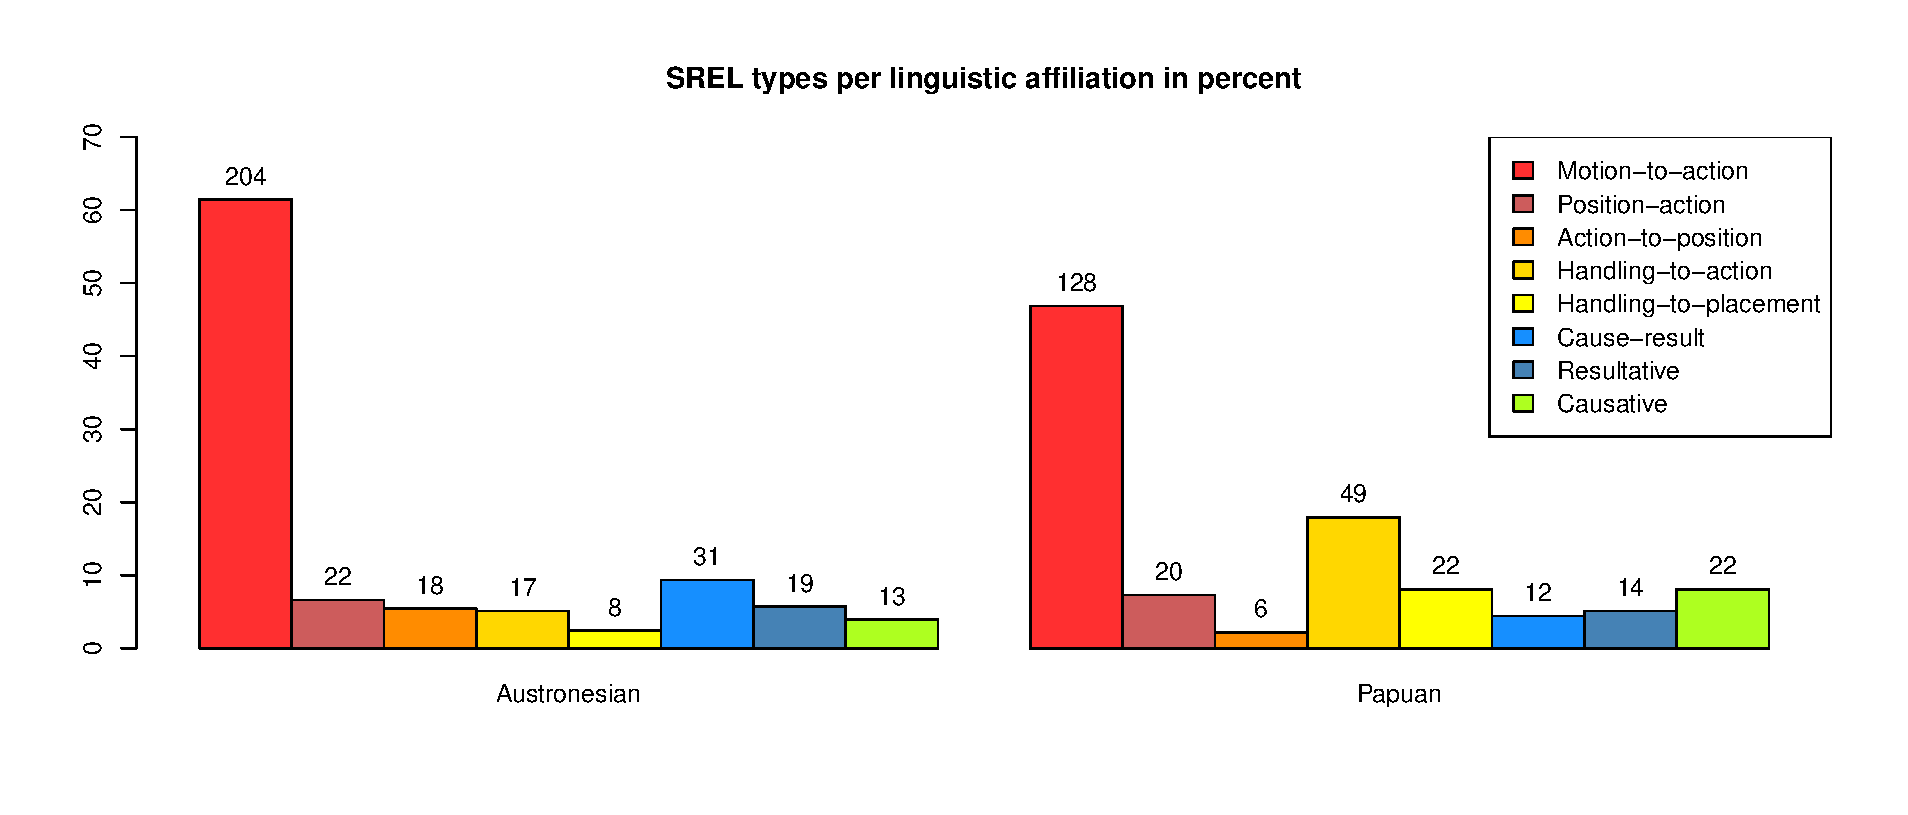
\includegraphics[width=\columnwidth]{figures/SREL_Family.eps}
\caption[SREL types per linguistic affiliation in percent]{SREL types per linguistic affiliation in percent. Numbers on top of the bars refer to the number of observations in the dataset.}\label{fig:srel-family}
\end{figure}
\begin{figure}[ht]
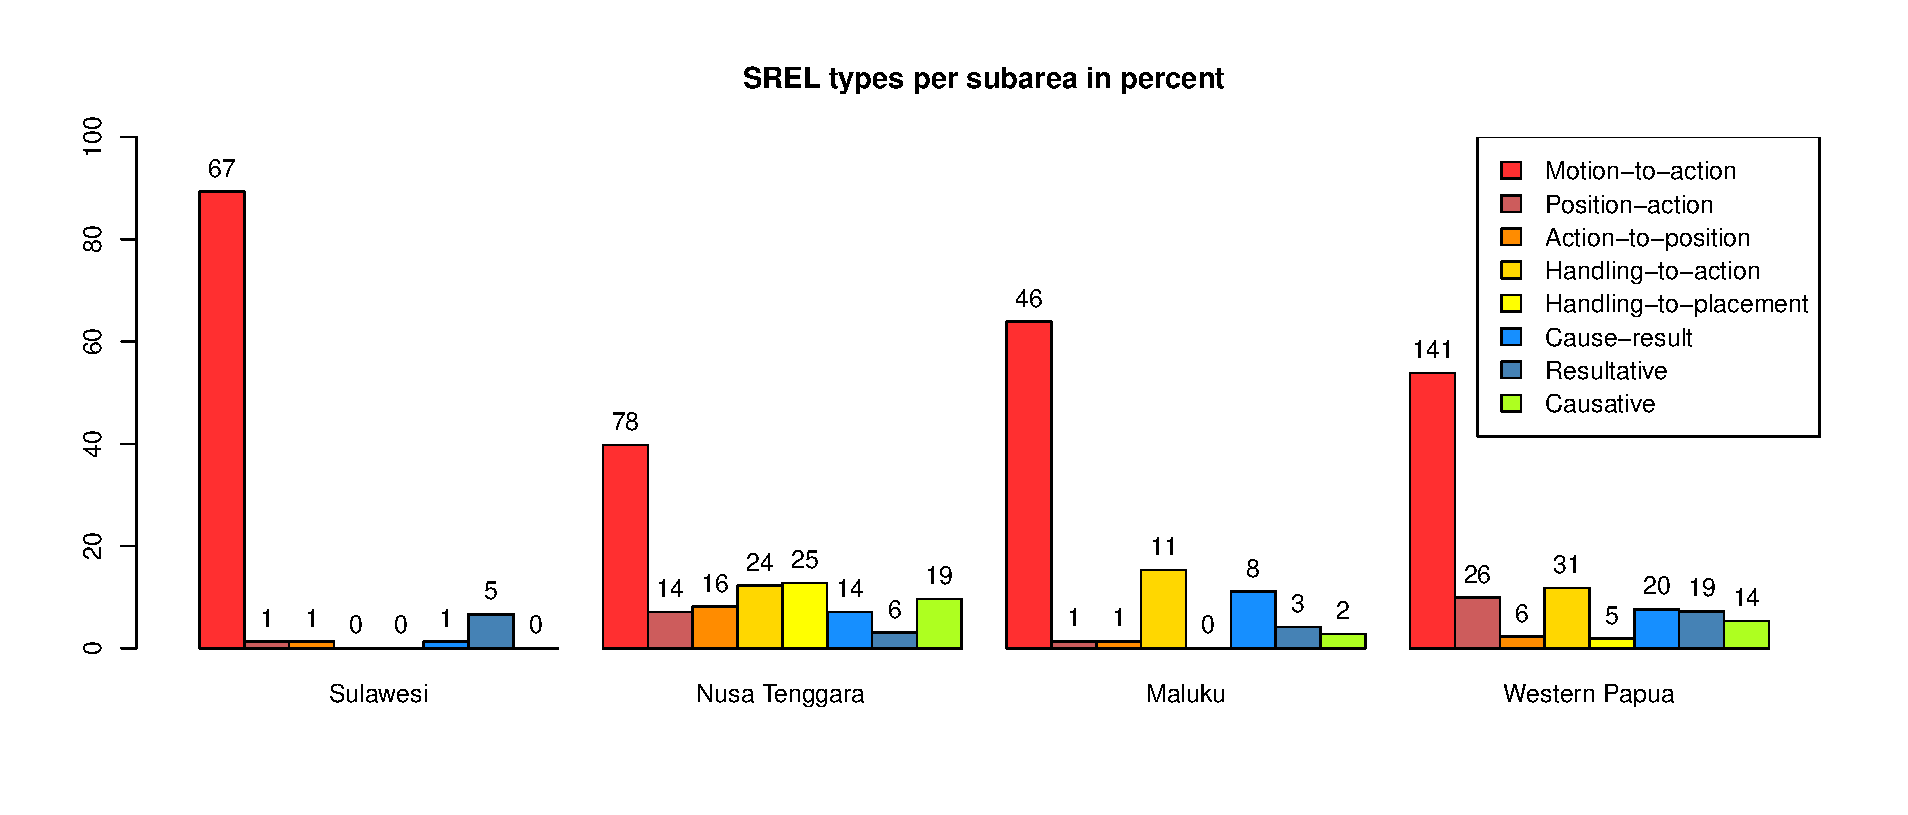
\includegraphics[width=\columnwidth]{figures/SREL_Group.eps}
\caption[SREL types per subarea in percent]{SREL types per subarea in percent. Numbers on top of the bars refer to the number of observations in the dataset.}\label{fig:srel-group}
\end{figure}

The areal distribution of \textsc{srel} constructions seems even more remarkable. The Sulawesi subarea is practically devoid of \textsc{srel}s, and only exhibits a high use of motion-to-action across all five languages, except Muna (with only two attested examples%; cf. also Table \ref{table:srel-language} below
). The only other \textsc{srel} construction that is in use is resultatives, but they are confined to two of the three south-eastern languages, Tolaki and Tukang Besi. The other three subareas all bear witness to a much higher diversity of \textsc{srel} constructions. As with the comparison of language family affiliation above, small differences are discernable from Figure \ref{fig:srel-group}. While Nusa Tenggara languages seem make good use of all other \textsc{srel} constructions, the Maluku languages appear to lack the two position-marking constructions, as well as handling-to-placement, which seems to be a defining feature of most Nusa Tenggara languages (in the Western Papua group, only Papuan languages show attested examples of this construction). Another minor \textsc{srel} construction that peaks in the Nusa Tenggara group is action-to-position. In Western Papua, we only have two languages with attested cases, of which all but one are from Wooi. Note that for this construction, both corpus languages, Waima'a and Wooi, contribute the bulk of instances. Another more general feature of the EI data%, as shown by Table \ref{table:srel-language}, 
is that most \textsc{srel} constructions, especially the major ones, clearly show an even distribution among a majority of EI languages. The position-marking constructions, on the other hand, are more unevenly distributed across the dataset, and thus warrant a more cautious treatment.

%\begin{table}
%\begin{scriptsize}
%\begin{tabular}{l r r r r r r r r}
%  \lsptoprule
%& \multicolumn{3}{c|}{orientation} & %\multicolumn{2}{c|}{handling} & %\multicolumn{3}{c}{causation} \\
% & {motion-to-action} & {position-action} & %{action-to-position} & {handling-to-action} & {handling-to-placement} & {cause-result} & {resultative} & {causative} \\ 
%  \hline
%  Muna &   2 &   0 &   0 &   0 &   0 &   0 &   0 &   0 \\ 
%  Pendau &  19 &   0 &   0 &   0 &   0 &   0 &   0 &   0 \\ 
%  Tajio &  18 &   0 &   0 &   0 &   0 &   0 &   0 &   0 \\ 
%  Tolaki &  18 &   1 &   0 &   0 &   0 &   0 &   1 &   0 \\ 
%  Tukang Besi &  10 &   0 &   1 &   0 &   0 &   1 &   4 &   0 \\ \hline
%  Abui &   9 &   1 &   0 & 4 & 2 & 0 & 0 &   4 \\ 
%  Alorese &  10 &   0 &   0 &   0 &   0 &   0 &   0 &   7 \\ 
%  Bunaq &   1 &   0 &   1 &   0 &   0 &   0 &   2 &   2 \\ 
%  Kaera &   1 &   0 &   0 &   2 &   5 &   0 &   0 &   2 \\ 
%  Kambera &   1 &   1 &   0 &   0 &   0 &   0 &   0 &   0 \\ 
%  Klon &  10 &   0 &   3 &   5 &   6 &   0 &   1 &   0 \\ 
%  Makalero &   3 &   0 &   0 &   2 &   2 &   2 &   0 &   0 \\ 
%  Teiwa &   9 &   9 &   0 &   6 &   1 &   2 &   0 &   2 \\ 
%  Tetun &   6 &   0 &   0 &   3 &   0 &   6 &   3 &   1 \\ 
%  Waima'a &  19 &   1 &   12 &   2 &   8 &   2 &   0 &  0 \\ 
%  Western Pantar &   9 &   2 &   0 &   0 &   1 &   2 &   0 &   1 \\ \hline
%  Buru & 16  &  0 & 0 & 0  & 0  &  3 & 0  &  2 \\
%  Selaru &   1 &   0 &   0 &   0 &   0 &   1 &   0 &  0 \\ 
%  Taba &   8 &   0 &   0 &   4 &   0 &   3 &   3 &  0 \\ 
%  Tidore & 14 & 1 & 0 & 7  & 0  &  1 &  0 & 0 \\
%  Tobelo &   7 &   0 &   1 &   0 &   0 &   0 &   0 & 0 \\ \hline
%  Abun &  14 &   0 &   0 &   0 &   0 &   0 &   0 &   1 \\ 
%  Biak &  11 &   5 &   0 &  0 &   0 &   11 &   3 &   1 \\ 
%  Dusner &  10 &   4 &   0 &   1 &   0 &   1 &   0 &   1 \\ 
%  Hatam &  14 &   0 &   0 &   7 &   2 &   0 &   0 &   0 \\ 
%  Inanwatan &   1 &   0 &   1 &   2 &   0 &   0 &   0 &   2 \\ 
%  Maybrat &   6 &   5 &   0 &   1 &   2 &   1 &   3 &   3 \\ 
%  Mor &  22 &   0 &   0 &   0 &   0 &   1 &   0 &   0 \\ 
%  Moskona &   8 &   2 &   0 &   7 &   1 &   2 &   5 &   5 \\ 
%  Mpur &  10 &   0 &   0 &   1 &   0 &   0 &   3 &   0 \\ 
%  Sougb &  12 &   0 &   0 &   5 &   0 &   2 &   0 &   0 \\ 
%  Wooi &  33 &  10 &   5 &   7 &   0 &   2 &   5 &   1 \\ 
%   \hline
%      Total & 332 & 42 & 24 & 66 & 30 & 43 & 33 & 35 \\
%   \hline
%\end{tabular}
%\end{scriptsize}
%\caption{Distribution of attested SREL construction types across the EI languages}
%\label{table:srel-language}
%\end{table}

The morphosyntactic patterns found with \textsc{srel} constructions also return a rather homogeneous picture when compared to the \textsc{mod} constructions from the last sections. Starting with referentiality values, we find that the values ``A", ``E", and ``X" hardly appear at all in \textsc{srel} constructions. The dominant pattern for orientation and handling constructions is ``S", while for \textsc{srel}s denoting causation, the "D" pattern is predominant. Action-to-position MVCs seem to cluster in this regard with causation rather than with orientation, and, as we shall see later, they arguably involve semantics of causation. Head marking in \textsc{srel} MVCs is also subject to variation across the different constructions. While the ubiquitous motion-to-action constructions may appear in any headedness pattern (both heads marked being the most frequent one, though), the other constructions seem to be more constrained. In most cases, the ``B" pattern is prevalent, followed by ``1" and ``S". However, neither handling construction is attested with a shared affix set (``S"). The less common patterns ``2" and ``N" only occur sporadically with most \textsc{srel}s. In terms of contiguity, the verbs in \textsc{srel} constructions are preferentially construed in tight sequence, with two exceptions. In both handling-to-action and handling-to-placement constructions, the value ``1" occurs more frequently than the ``C" value. This reflects the transitive nature of the first verb in such constructions, as the object of the \textsc{handling} verb is typically expressed by a full NP before the following V$_2$, at least in AVO languages.

\begin{table}
\centering
\begin{tabular}{rrrrrr}
  \lsptoprule
Referentiality & S & SO & D & A & X \\ 
  \hline
  motion-to-action & 326 &   3 &   2 &   1 &   0 \\ 
  position-action &  42 &   0 &   0 &   0 &   0 \\ 
  action-to-position &  11 &   0 &  11 &   0 &   2 \\ 
  handling-to-action &  55 &   9 &   2 &   0 &   0 \\ 
  handling-to-placement &  24 &   5 &   1 &   0 &   0 \\ 
  cause-result &  18 &   6 &  18 &   0 &   1 \\ 
  resultative &   5 &   1 &  26 &   0 &   1 \\ 
  causative &   9 &   0 &  26 &   0 &   0 \\ 
   \hline
 \\
  \hline
Headedness & B & 1 & 2 & S & N \\ 
  \hline
  motion-to-action & 144 &  26 &  24 &   9 &  22 \\ 
  position-action &  23 &   3 &   0 &   1 &   2 \\ 
  action-to-position &   6 &   0 &   0 &   2 &   0 \\ 
  handling-to-action &  32 &   3 &   1 &   0 &   6 \\ 
  handling-to-placement &   5 &   0 &   0 &   0 &   0 \\ 
  cause-result &  14 &  11 &   0 &   1 &   0 \\ 
  resultative &  10 &   7 &   0 &  10 &   0 \\ 
  causative &  10 &   0 &   0 &   3 &   0 \\ 
   \hline
 \\
  \hline
Contiguity & W & C & 1 & 2 & 3 \\ 
  \hline
  motion-to-action &  12 & 261 &  55 &   3 &   1 \\ 
  position-action &   0 &  32 &   9 &   1 &   0 \\ 
  action-to-position &   1 &  17 &   5 &   1 &   0 \\ 
  handling-to-action &   2 &  23 &  35 &   4 &   2 \\ 
  handling-to-placement &   0 &   7 &  18 &   5 &   0 \\ 
  cause-result &   2 &  33 &   7 &   1 &   0 \\ 
  resultative &   0 &  19 &  13 &   1 &   0 \\ 
  causative &   3 &  20 &  12 &   0 &   0 \\ 
   \lspbottomrule
\end{tabular}
\caption[Morphosyntactic properties of \textsc{srel} constructions]{Morphosyntactic properties of \textsc{srel} constructions in EI. Table components from top to bottom refer to referentiality (see §\ref{sec:argumentstructure}), headedness (see §\ref{sec:headedness}), and contiguity (see §\ref{sec:contiguity}), respectively.}
\label{table:SREL_formal}
\end{table}

The subsequent sections turn to the \textsc{srel} constructions and provide examples.

\subsection{Orientation} \label{sec:orientation}
\subsubsection{Motion-to-action} \label{sec:motion-to-action}

Motion-to-action constitutes the only MVC type found in all EI languages investigated, and can therefore be regarded as the prototypical MVC in Eastern Indonesia. This is a surprising result given that this construction appears not to have received major attention in the serialisation literature. Instances of motion-to-action have two slots, a \textsc{motion} slot followed by an \textsc{action} slot, each of which my be filled recursively with another MVC. Table \ref{table:motion-to-action} illustrates the distributional properties of motion-to-action in the EI area.

\begin{table}
\begin{tabular}{ll}
\lsptoprule
Feature&Value\tabularnewline
\hline
Template&V1 \textsc{motion verb} -- V2 \textsc{action verb}\tabularnewline
No. of attested instances& 332/2146 \tabularnewline
No. of attested languages& 32/32 \tabularnewline
Distribution across areas& \textsc{sul} (5/5), \textsc{nus} (11/11), \textsc{mal} (5/5) \textsc{pap} (11/11) \tabularnewline
Distribution across families& \textsc{pap} (16), \textsc{aus} (16) \tabularnewline
\lspbottomrule
\end{tabular}
\caption[Template and basic distribution of motion-to-action MVCs]{Template and basic distribution of motion-to-action MVCs in the EI sample.}
\label{table:motion-to-action}
\end{table}

The following examples illustrate motion-to-action cases from the different subareas. As can be seen, the motion stage always comes first, and leads up to a second stage in which some action is carried out by the actor. The motion slot in V$_1$ is typically filled by a directed path verb, such as \textsc{come} or \textsc{go} (as in example (\ref{Tajio_18}) from Tajio), but may also host a range of other motion verbs, for instance vertical path verbs (as in example (\ref{Buru_12}) from Buru), punctual contained-path verbs like \textsc{enter} in (\ref{Western_9}) from Western Pantar, or semantically more specific verbs as \textit{mbur} in the Dusner example in (\ref{Dusner_45}) (\textit{mbur} is variously glossed as `leave' or `go home'). The verbs participating in motion-to-action constructions may either all bear inflection (as in the Tajio example), or none of the verb takes inflection (the Western Pantar and Buru cases). In some languages like Hatam, only the motion verb in V$_1$ is inflected. Even rarer is the inflectional pattern found in Inanwatan where the second verb is the locus of inflection, and the motion verb is preposed to it (see also below). Shared affix sets are quite uncommon with motion-to-action, and even languages that allow for this coding type in other MVCs refrain from using it with motion-to-action (for example, Tukang Besi).

\ea \label{Tajio_18}
\langinfo{Tajio}{Austronesian, WMP}{\citealt[294]{mayani2013grammar}}\\
\glll sia’u jo majaok mongulam \\
sia’u jio mV-jaok moN-ulam \\
1\textsc{sg} \textsc{neg} \textsc{st}.\textsc{nrls}-come \textsc{av}.\textsc{nrls}-cure \\
\glft `I will not come to cure (you).’\\ 
\z

\ea \label{Western_9}
\langinfo{Western Pantar}{Papuan, TAP}{\citealt[81]{holton2014western}}\\
\gll wakke bogga gai aname ging aukung banang \\
child young.man 3\textsc{sg}.\textsc{poss} person 3\textsc{pl}.\textsc{act} enter ask \\
\glft `The young man's people go in and ask.'\\ 
\z

\ea \label{Buru_12}
\langinfo{Buru}{Austronesian, CMP}{\citealt[209]{grimes1991buru}}\\
\gll sira te keha baga saka huma lale-n moo \\
3\textsc{pl} \textsc{abil} ascend sleep up house inside-\textsc{gen} \textsc{neg} \\
\glft `They can't go up and sleep inside the [pile] house.'\\ 
\z

\ea \label{Dusner_45}
\langinfo{Dusner}{Austronesian, SHWNG}{\citealt[52]{dalrymple2012}}\\
\glll ndombur na rau ro ran rine ye ndoton e ro \\
ndo-mbur ra rau ro ran ri-ne ye ndo-ton e ro \\
1\textsc{in}.\textsc{pl}-leave move seaward at sago \textsc{evid}-\textsc{dem}.\textsc{prx} \textsc{fill} 1\textsc{in}.\textsc{pl}-sit \textsc{fill} at \\
\glft `We went on seaward to the sago trees where we stayed.'\\ 
\z

It becomes clear from these examples that the action slot does not only permit dynamic verbs. Rather, what seems crucial is that the moving referent is the willful instigator of the action to take place at the place of destination. That is, the stage of sleeping in the Buru example from (\ref{Buru_12}) is planned or intended by the group of referents to take place after they reach the pile house. And in example (\ref{Dusner_45}) from Dusner, the staying is part of the event schema in much the same way, and is interpreted to motivate the change of place denoted by the forerunner motion stage.

Let us now turn to more complex examples. As I said, motion-to-action MVCs appear to allow the construal of stacked MVCs in either of their slots. Example (\ref{Tetun002}) from Tetun Fehan shows a motion complex MVC in initial position followed by a single verb, \textit{hasoru}, in the action slot. Example (\ref{KYO003}) from Klon illustrates the opposite case: Here, the action slot of a motion-to-action construction hosts another MVC (note that Klon has APV word order and places locative verbs in construction-initial position so that the action slot is here filled by a construction [\textsc{locative} \textsc{action}]). Both options of stacked MVCs are attested in a range of EI languages, though not in all. What is licit within a given slot thus seems to be first and foremost a result of language-specific rules.

\ea \label{Tetun002}
\langinfo{Tetun Fehan}{Austronesian, CMP}{\citealt[172]{vanklinken1999grammar}}\\
\gll ha'u k-sai mai k-asoru nia \\
\textsc{1}\textsc{sg} \textsc{1}\textsc{sg}-exit come \textsc{1}\textsc{sg}-meet \textsc{3}\textsc{sg} \\
\glft `I came out and met him.'\\ 
\z

\ea \label{KYO003}
\langinfo{Klon}{Papuan, TAP}{\citealt[148]{baird2008grammar}}\\
\gll hle onon uqlilik, bo leer ga ma, bo waa qad Koilal Marka g-hoi \textbf{qad} amai alol \textbf{mi} \textbf{ted} \\
Kui \textsc{pl} vengeful \textsc{seq} ruler \textsc{3}.\textsc{act} come \textsc{seq} go come Koilal Marka \textsc{3}.\textsc{ug}-order come below harbour be.at sail \\
\glft `The Kui were vengeful so the ruler came, then came and went and ordered Koilal Marka to come sail below in the harbour.'\\ 
\z

Some Papuan languages have only very few or even just one attested example for motion-to-action. This is the case in Bunaq and Inanwatan. The number of attested case remained low even after a search of the appended texts of the respective data sources. We would therefore need to assume that, although motion-to-action construals are probably available in all EI languages one way or another, such construals differ considerably in the extent to which they are used in natural speech. While speakers of some languages put motion-to-action MVCs to good use in all kinds of speech contexts (for instance in Wooi), speakers of other languages like Bunaq or Inanwatan tend not to compress motion and action sequences into the shape of a clause (or better, an IP). The following examples show the only attested cases of motion-to-action for Bunaq and Inanwatan, all of which are but dubious members of motion-to-action. Example (\ref{Bunaq_60}) is the only example that I annotated as a potential case of motion-to-action in Bunaq. It is ambiguous between a translational motion interpretation (keep on going to (the garden) and clear undergrowth) and a grammaticalised aspectual reading (keep on clearing undergrowth), but as the example occurs in \citet[463]{schapper2009bunaq} right after another example with \textit{mal ciluq} that obviously denotes translational motion, I tentatively interpret it as motion-to-action. If this indeed belongs to the group of motion-to-action MVCs, it is one of only a handful of examples in which the order of motion and action is inverted. If \textsc{srel} MVCs are defined as always retaining the iconicity of the event sequence, then this example would need to be dropped. In the text sample appended to Schapper's grammar I only came across one more utterance that bears a resemblance to motion-to-action. The placement of a comma, however, prevented me from adding (\ref{Bunaq_n1}) to the EI dataset. Another feature that would hint at a less tight construal is the use of two different aspectual operators, each targeting one of the verbs. This is unsual even for two-stage MVCs that at times allow the temporal modification of only one event stage (think again of the introductory example (\ref{WMH_Julio_goat099}) from Chapter \ref{ch:sem} where the placement of the aspctual \textit{lo} was right after the motion verb, and not after the whole motion-to-action construction). Example (\ref{Inan_20}), finally, is the only case of motion-to-action that I found in \citet{devries2004}. At the matrix level, two constituents are juxtaposed: \textit{mé-iqo-rita-re} and \textit{mo-wé-tira-rita-i}. The second constituent again forms a MVC, and shows the by-now familiar construal of Inanwatan 'complex phrasal verbs' (cf. \citealt[57]{devries2004}) with a bare verb (in this case the motion verb) preposed to an inflected V$_2$ that takes an object indexing prefix and a set of suffixes denoting TAM and subject number and gender. Note that although Inanwatan is strictly AOV, the order of the verbs still follows the temporal order of event stages.

\ea \label{Bunaq_60}
\langinfo{Bunaq}{Papuan, TAP}{\citealt[463]{schapper2009bunaq}}\\
\gll u t-ul mal ciluq \\
undergrowth 3\textsc{inan}-pull go rest \\
\glft ‘(They) keep going to clear undergrowth.’\\
\z

\ea \label{Bunaq_n1}
\langinfo{Bunaq}{Papuan, TAP}{\citealt[512]{schapper2009bunaq}}\\
\gll rebel si, g-ota gie \\
descend \textsc{rls} 3\textsc{an}-stab \textsc{prosp} \\
\glft ‘(They) would go down to stab (them).’\\ 
\z

\ea \label{Inan_20}
\langinfo{Inanwatan}{Papuan, SBH}{\citealt[85]{devries2004}}\\
\gll sudah mai mé-iqo-rita-re mo-wé-tira-rita-i, tígo mao-go mé-ra-rita-i \\
so this.\textsc{f} 3\textsc{sg}-put.down-\textsc{dur}-\textsc{pst}.\textsc{pl} come-3\textsc{sg}-take-\textsc{dur}-\textsc{pst}.\textsc{pl} so wife-\textsc{circ} 3\textsc{sg}-take-\textsc{dur}-\textsc{pst}.\textsc{sg}.\textsc{m} \\
\glft `So they put her down and he came and took her to become his wife.'\\ 
\z

\subsubsection{Position-action}\label{sec:position-action}

Position-action MVCs combine a posture verb in V$_1$ with an action verb in V$_2$. It is the only construction in the \textsc{srel} constructional family that does not produce a reading of two successive spatio-temporal stages, but invokes an interpretation of two events going on at the same time. The acting participant assumes a certain position (and, at least in case of \textsc{sit} and \textsc{stand} verbs, invests energy to maintain this position), while performing some action at the same time. I regard such construals as two-stage nonetheless with the only difference that the event stages overlap in space and time. The question whether or not two situations that overlap in space and time constitute one and the same event has been raised in formal semantics, but a one-event conclusion has been dismissed as too narrow a definition of eventhood (see e.g. \citealt{maienborn2005limits} for discussion). Therefore we may assume that two event arguments, licensed by two LLEs, may refuse merging although they are interpreted as happening at the same time and place. As Table \ref{table:position-action} illustrates, position-action MVCs are only sparsely distributed over the EI region (with attested examples in 12 languages). Both Sulawesi and Maluku hardly show any usage at all (one attested example each), and in the two other subareas, it is only some languages that make regular use of it.

\begin{table}
\begin{tabular}{ll}
\lsptoprule
Feature&Value\tabularnewline
\hline
Template&V1 \textsc{posture verb} -- V2 \textsc{action verb}\tabularnewline
No. of attested instances& 42/2146 \tabularnewline
No. of attested languages& 12/32 \tabularnewline
Distribution across areas& \textsc{sul} (1/5), \textsc{nus} (5/11), \textsc{mal} (1/5) \textsc{pap} (5/11) \tabularnewline
Distribution across families& \textsc{pap} (6), \textsc{aus} (6) \tabularnewline
\lspbottomrule
\end{tabular}
\caption[Template and basic distribution of position-action MVCs]{Template and basic distribution of position-action MVCs in the EI sample.}
\label{table:position-action}
\end{table}

Here are some typical examples from languages with more than one attested example: Teiwa in the Nusa Tenggara group, Maybrat and Wooi in the Western Papua group. According to Table \ref{table:SREL_formal} from §\ref{sec:stage-relating}, prototypical position-action constructions have shared subject arguments (``S"), both verbs are inflected (``B"), and the verbs are placed adjacent to each other (``C"). In case V$_2$ has a transitive verb with a full object NP, this would lead in AOV languages to an NP placement between the position verb and the action verb, as in example (\ref{Teiwa_24}) from Teiwa. There are three posture verbs that may be found in the position slot: \textsc{sit} verbs, as in example (\ref{Teiwa_24}) from Teiwa, and \textsc{stand} verbs, as in (\ref{Maybrat_75}) and (\ref{WBW016}), occur most frequently, but occasional examples with \textsc{lie} verbs are attested for Biak, Moskona, and Wooi (all belonging to the Western Papua subarea). While the Teiwa example illustrates a basic positon-action construction consisting of just two verbs, the examples from Maybrat and Wooi both show complex construals in which the action slot hosts another MVC. In example (\ref{Maybrat_75}) we encounter a three-verb string, denoting three event stages: a position stage, a handling stage, and, finally, a placement stage. As handling-to-placement MVCs recur in a number of languages, I propose that they constitute a stage-relating MVC type of their own (see §\ref{sec:handling-to-placement} below). In this case, it seems as if the action slot of a position-action construction is filled with a handling-to-placement MVC. This is the only way the string can be resolved without violating the handling-to-placement template that requires a handling verb in V$_1$. The Wooi case in (\ref{WBW016}) illustrates another stacked MVC with a position-action construction at the matrix level. Here, it is a direction complex MVC, consisting of three verbs \textit{hayo} `watch', \textit{tuva} `go.after' and \textit{ra} `go', that enters the action slot. I have not come across MVCs filling the position slot of position-action constructions, though.\footnote{The only potential combination that would not be semantically odd is, I think, a locative case-marking MVC embedded into the position slot of position-action, thus yielding something like \textit{Jones \textbf{sit} \textbf{be} in bathroom \textbf{butter} toast}. Such a combination, however, is not attested in the dataset. Another potential combination, action-to-position plus position-action, seems to be at odds with the constructional meanings, as the former mostly denotes an object that is brought into a certain position by some action. Action-position-action would then involve a participant in object function that is placed somewhere, and only then performs (now in subject function) some action - a setting that would be quite uncommon by all accounts.}

\ea \label{Teiwa_24}
\langinfo{Teiwa}{Papuan, TAP}{\citealt[309]{klamer2010grammar}}\\
\gll a yix-in si, ga-gasqai ga'an atab un mis-an qar tapan pati \\
3\textsc{sg} descend-\textsc{rls} \textsc{sim} 3\textsc{sg}-sister 3\textsc{sg} truly \textsc{cont} sit-\textsc{rls} rice pound \textsc{prog} \\
\glft `While he went down, his sister [was] actually still sitting pounding rice.'\\ 
\z

\ea \label{Maybrat_75}
\langinfo{Maybrat}{Papuan, isolate}{\citealt[215]{dol2007grammar}}\\
\gll y-ros y-o y-ati ara a \\
3\textsc{m}-stand 3\textsc{m}-take 3\textsc{m}-put.in.ground tree \textsc{int} \\
\glft 1. `Does he stand and take and put the sticks into the ground?' \\ 2. `He stands and takes (the sticks), but should he put them into the ground (or should he do something else with them)?'\\
\z

\ea \label{WBW016}
\langinfo{Wooi}{Austronesian, SHWNG}{WBW\_pear\_Agus}\\
\glll henda kutua mara trus ce heyo tuva hnia ra mara \\
he-ra kutu-a mara trus $<$i$>$tera $<$i$>$hayo tuva hnia ra mara \\
\textsc{3}\textsc{pl}-go cut-\textsc{obj}.\textsc{nsg} \textsc{seq} then $<$\textsc{3}\textsc{sg}$>$stand $<$\textsc{3}\textsc{sg}$>$watch go.after \textsc{3}\textsc{pl} go \textsc{seq} \\
\glft `He stood and watched them passing as they went past him.'\\ 
\z

Example (\ref{Maybrat_75}) above also illustrates another property of position-action in Maybrat. If an interrogative marker is added to the construction, it may either target the whole matrix MVC, or just the last event stage that is adjacent to the clause-final marker. This behaviour thus mirrors the criterion of partial temporal modification that I suggested in §\ref{sec:criteria_mvcs} to be a defining characteristic of \textsc{srel}s.

One example with a reversed order action -- position was found in Teiwa as well. I suppose that \textit{ga-boxan tas} in (\ref{Teiwa002}) can be considered a lexicalised combination rather than a regular example of position -- action.

\ea \label{Teiwa002}
\langinfo{Teiwa}{Papuan, TAP}{\citealt[314]{klamer2010grammar}}\\
\gll rai na-soi ga-kamadal ga-boxan tas \\
king \textsc{1}\textsc{sg}-order \textsc{3}\textsc{sg}-belt \textsc{3}\textsc{sg}-guard stand \\
\glft `The king ordered me to guard his belt.'\\ 
\z

\subsubsection{Action-to-Position}\label{sec:action-to-position}

Action-to-position instances consist of an action stage followed by a positional stage. The second stage may either be a posture verb, specifiying the spatial alignment of some object, or a stative positional verb, stressing a non-dynamic resultant phase after the action stage has come to an end. Action-to-position is confined to only 24 cases from seven languages, from all subareas. Its distribution is hard to trace as there are so little data, but it seems that, by looking at the data points per language, the number of occurrences can be increased by searching through larger language corpora, as the number of cases from Waima'a and Wooi illustrates. The frequency of action-to-position in EI natural speech data seems at any rate to be rather low. Table \ref{table:action-to-position} presents the basic numbers.

\begin{table}
\begin{tabular}{ll}
\lsptoprule
Feature&Value\tabularnewline
\hline
Template&V1 \textsc{action verb} -- V2 \textsc{posture/positional verb}\tabularnewline
No. of attested instances& 24/2146 \tabularnewline
No. of attested languages& 7/32 \tabularnewline
Distribution across areas& \textsc{sul} (1/5), \textsc{nus} (3/11), \textsc{mal} (1/5) \textsc{pap} (2/11) \tabularnewline
Distribution across families& \textsc{pap} (4), \textsc{aus} (3) \tabularnewline
\lspbottomrule
\end{tabular}
\caption[Template and basic distribution of action-to-position MVCs]{Template and basic distribution of action-to-position MVCs in the EI sample.}
\label{table:action-to-position}
\end{table}


Action-to-position MVCs fall into two subtypes, as stated above: (i) action-to-posture, and (ii) action-to-positional state. For lack of data, I tentatively included both subtypes under one constructional schema, but they may in fact constitute related but different constructions. The former variant is attested in most of the languages that have action-to-position. Consider the following examples. In example (\ref{Waimaqa_65}) from Waima'a and example (\ref{Tobelo_20}) from Tobelo a participant is pulled into upright position. The construction involves a verb of pulling complemented by a \textsc{stand} verb in V$_2$. Example (\ref{Wooi_86}) from Wooi illustrates another posture verb in V$_2$. Here, the object referent is brought into a horizontal lying position (\textsc{lie} verbs are in fact only attested in Wooi). Note that the referential expression of such construals needs to have a shift in syntactic function: the direct object of V$_1$ is to become the subject of V$_2$, as exemplified by the Wooi case in (\ref{Wooi_86}). What is interesting with the first two examples is that although such a reference shift arguably takes place on the logical-conceptual level, the formal encoding of the referential expressions does not exactly follow this shift. Rather, in the Waima'a case, we observe a referential shift from the boy's arm (the object of V$_1$) to the boy now being understood as the referent that is moved to a standing position (since it is not just the boy's arm that is supposed to stand as a result of the event). A similar shift takes place in the Tobelo example. Here, the referent being pulled up is expressed by a third person object prefix on the first verb, yet on the posture verb the same referent is referred to with a second person subject indexer. Such person shifts are not uncommon in the languages of the Melanesian region, and are used to highlight prominent parts of natural speech contexts, for instance in story narration (see \citealt{margetts2015person} for a recent account of person shifts in Saliba-Logea). Discourse structure in such contexts shapes the grammatical expression of referents. This is another interesting case of unreliable morphology where the formal encoding of referential expression does not lead to a disambiguation of internal MVC structure.

\ea \label{Waimaqa_65}
\langinfo{Wama'a}{Austronesian, CMP}{pear\_Bendita 030}\\
\gll sik ale'e askai ke lime nini nhii ulo \\
grab child male \textsc{dem} arm \textsc{poss} stand already \\
\glft `They grabbed the boy's hand (to help him) get
up.'\\ 
\z

\ea \label{Tobelo_20}
\langinfo{Tobelo}{Papuan, NH}{\citealt[63]{holton2003tobelo}}\\
\gll t-a-ika t-i-tauru no-maoko la no-ma-tagi \\
1-vf-\textsc{all} 1-3\textsc{m}-pull 2-stand \textsc{conj} 2-\textsc{refl}-walk \\
\glft `I pulled him up so that he could walk' (lit. I pull him you stand...)\\ 
\z

\ea \label{Wooi_86}
\langinfo{Wooi}{Austronesian, SHWNG}{midwife\_traditional\_medicine}\\
\glll heton via topi ning ma heteng kepan \\
he-ong $<$i$>$va topi ning ma he-eng kepang \\
3\textsc{pl}-put $<$3\textsc{sg}$>$lie like this \textsc{top} 3\textsc{pl}-sleep overlap \\
\glft `Preparing it (the leaves) like this they sleep on it.' (lit. putting it lie like this, they sleep on it) \\ 
\z

As \textit{va(ta)} `lie' may also convey durative semantics in Wooi, the Wooi case in (\ref{Wooi_86}) straddles the dividing line between both subtypes of action-to-position. This becomes obvious in examples such as the following where the pig assumes a lying position only as a result of its being dead. In my understanding, the main semantic contribution of \textit{vata} in such cases is that it translates into an aspectual notion of durative resultant state, something like `die and remain (lying) there for some time'.

\ea \label{}
\langinfo{Wooi}{Austronesian, SHWNG}{MANTERA\_magic\_charms}\\
\glll asurang vat keria viata \\
asurang vati $<$i$>$karia $<$i$>$vata \\
pig \textsc{det}:\textsc{sg} $<$3\textsc{sg}$>$-die $<$3\textsc{sg}$>$-lie \\
\glft `(After slashing it with a machete) the pig dies.'\\ 
\z

Similar cases in which V$_2$ introduces some kind of stative resultant stage are found in Waima'a. Consider example (\ref{WMHP136}) below with a \textsc{stay} verb in final position, probably specifying that the placement of the basket on the bicycle has been successfull, and that it would remain there.

\ea \label{WMHP136}
\langinfo{Waima'a}{Austronesian, CMP}{pear\_Carlito 140}\\
\gll ne boten mai tese hite n'au biskalta oon \\
\textsc{3}\textsc{sg} basket come place \textsc{ptl} stay bicycle above \\
\glft `His basket, (they) came putting it onto (his) bicycle.' \\ 
\z

There is a very small number of further constructions that seem similar to action-to-position constructions, but have a rather specific stative verb in V$_2$ position. Example (\ref{MOSK001}) from Moskona is such a case. More data would be helpful in order to gain a clearer picture on such constructions.

\ea \label{MOSK001}
\langinfo{Moskona}{Papuan, EBH}{\citealt[295]{gravelle2010grammar}}\\
\gll ofa eyta meber efifr-ef \\
s/he take shelf level-near \\
\glft ‘He made the shelf [so] it is level.’\\ 
\z

\subsection{Handling}

In the last sections, we have seen stage-relating constructions that in some way or another contribute information on the spatial setting of events. Motion-to-action motivates a shift from one location to another by entailing that the moving actor is moving with some clear intention. Motion-to-action thus helps shift the discourse scene in story telling. \textsc{srel} constructions involving positional verbs provide information on stative spatial orientation of some participant, either specifying the body posture of some acting participant, or the resting position of some manipulated object. 

Handling constructions are quite different and focus on the manual manipulation of objects, and what actions follow from them. Just as in orientation \textsc{srel}s, there is normally a strong implication of intentional acting entailed in handling \textsc{srel}s. I distinguish between two constructions: Handling-to-action and handling-to-placement. 

\subsubsection{Handling-to-action} \label{sec:handling-to-action}

Handling-to-action combines an event stage of manual object handling with a subsequent action stage. Prototypical instances are combinations of a \textsc{take} verb followed by some dynamic action verb in V$_2$. Handling-to-action is the secondmost frequent \textsc{srel} construction found in the EI sample after motion-to-action. Its distribution seems limited to Nusa Tenggara, Western Papua, and parts of the Halmahera archipelago. In both Nusa Tenggara and Western Papuan languages, the construction occurs in most languages of the sample, though its distribution is skewed towards Papuan languages. Table \ref{table:handling-to-action} presents the distributional numbers.

\begin{table}
\begin{tabular}{ll}
\lsptoprule
Feature&Value\tabularnewline
\hline
Template&V1 \textsc{handling verb} -- V2 \textsc{action verb}\tabularnewline
No. of attested instances& 66/2146 \tabularnewline
No. of attested languages& 17/32 \tabularnewline
Distribution across areas& \textsc{sul} (0/5), \textsc{nus} (7/11), \textsc{mal} (2/5) \textsc{pap} (8/11) \tabularnewline
Distribution across families& \textsc{pap} (12), \textsc{aus} (5) \tabularnewline
\lspbottomrule
\end{tabular}
\caption[Template and basic distribution of handling-to-action MVCs]{Template and basic distribution of handling-to-action MVCs in the EI sample.}
\label{table:handling-to-action}
\end{table}

Handling-to-action MVCs conform to the dominant headedness pattern in that both verbs inflect for verbal categories (disregarding the cases of unreliable morphology in Nusa Tenggara), but they slightly deviate in the other two morphosyntactic categories, referentiality and contiguity. As opposed to most other MVCs, handling-to-action MVCs predominantly have one constituent placed between their verbs. This is typically the direct object NP of the handling verb. In terms of referential interaction, one might expect the number of ``SO" cases (that is, the verbs share subject \emph{and} object) to be quite high because taking something and manipulating it would require such a referential coding. Yet, Table \ref{table:SREL_formal} from §\ref{sec:stage-relating} reveals that only a small fraction of cases indeed shows "SO" referential interaction. Most cases exhibit the much more common pattern ``S" where the subject but not the object is shared among the verbs. This is due to the fact that in most instances of handling-to-action, the handling verb introduces an object referent that is then understood as the instrument rather then the theme of the action denoted by the second verb. 

This brings up a further problem: how to distinguish between two-stage handling-to-action MVCs on the one hand, and one-stage instrumental case-marking MVCs on the other. A thorough testing would necessarily involve the criteria sketched in §\ref{sec:criteria_mvcs}. As this was not always possible, I assumed all instances in which \textsc{take} verbs (or related verbs of handling) in V$_1$ combine with verbs denoting manual action to be two-stage MVCs rather than modifying MVCs. This was backed by two assumptions: first, grammaticalised instrument-marking MVCs would probably also comprise cases of rather abstract instrument assignments with concrete manual action being semantically odd. However, all retrieved cases of handling-to-action still denote concrete manual action. And second, no change in constituent order was detected, also pointing to the conclusion that handling-to-action rather constitutes a two-stage event schema, and is constrained by the principle of temporal iconicity. Note that the cases of instrument \textsc{mod}s, as discussed in §\ref{sec:case-marking}, do show variable constituent order, and other properties that lend themselves to an analysis as somewhat grammaticalised instrument-marking constituent.

Let us now first have a look at this major group of instrument-introducing constructions. Consider the following examples. Example (\ref{Abui_103}) from Abui is a prototypical handling-to-action construction, with a \textsc{take} verb in V$_1$ and a subsequent action stage. The theme object of \textit{mi} is interpreted as the instrument that is used to perform the action of cutting wood (note that \textit{kawen} is moved here to a clause-initial focus position). In (\ref{Klon_87}) from Klon, a similar construal is used, but the verb translates as holding, not taking. I am assuming for the time being that such MVCs still form two-stage event construals (either by denoting a precursor stage to obtain the instrument, or in the sense of overlapping stages, as in the position-action construction discussed in §\ref{sec:position-action}). Example (\ref{Hatam_30} from Hatam is a similar case from the Western Papua subarea.

\ea \label{Abui_103}
\langinfo{Abui}{Papuan, TAP}{\citealt[386]{kratochvil2007grammar}}\\
\gll kawen ama mi bataa tukong \\
machete person take wood cut \\
\glft `With machete one cuts wood.'\\ 
\z

\ea \label{Klon_87}
\langinfo{Klon}{Papuan, TAP}{\citealt[146]{baird2008grammar}}\\
\gll gi-doqom ge eneem biasa ini puin iwi we~wei\\
3\textsc{poss}-grandfather 3\textsc{poss} tall.grass usual 3\textsc{nsg} hold house \textsc{rdp}~roof\\
\glft `They usually use his grandfather's tall grass to roof houses.'\\ 
\z

\ea \label{Hatam_30}
\langinfo{Hatam}{Papuan, Hatam-Mansim}{\citealt[101]{reesink1999grammar}}\\
\gll dani di-ba singau riu nab \\
I 1\textsc{sg}-take knife pierce pig \\
\glft `I pierced the pig with a knife.'\\ 
\z

Example (\ref{Hatam_30}) above is in fact not the only way to construe instrument-introducing MVCs in Hatam. In order to explicitly track the instrument argument, an instrument prefix may be used on the second verb. Here is another example from Hatam, showing the use of two homophonous, possibly related, prefixes. The instrument \textit{bi} denotes that the theme object of the preceding verb is interpreted as the instrument of the verb \textit{bi-} is attached to. The second \textit{bi-}, on the other hand, marks purposive relations between two predicates. Note that the placement of the subject indexers distinguishes both prefixes, as the former stands between the indexer and the verb root, while the latter precedes both indexer and verb root.

\ea \label{}
\langinfo{Hatam}{Papuan, Hatam-Mansim}{\citealt[101]{reesink1999grammar}}\\
\gll yoni i-ba micim i-bi-dat dani bigom bi-di-mai \\
they 3\textsc{pl}-take spear 3\textsc{pl}-\textsc{ins}-pierce I almost \textsc{purp}-1\textsc{sg}-die \\
\glft `They almost killed me with their spear(s).'\\ 
\z

Turning to the second group of handling-to-action cases, we can see that there is hardly any difference in construal, at least if the language in question does not overtly mark instruments, as we have seen in the Hatam case above. Take example (\ref{Kaera_7}) from Kaera as an illustration.

\ea \label{Kaera_7}
\langinfo{Kaera}{Papuan, TAP}{\citealt[136]{klamer2014kaera}}\\
\gll gang g-iya-t gang ge-sil tuning met or-i sei \\
3\textsc{sg} 3\textsc{sg}-go.down-\textsc{ipfv} 3\textsc{sg} 3\textsc{sg}-rope placenta take hang-\textsc{prfv} \textsc{compl} \\
\glft `Giving birth, she took his umbilical cord [and] hung [it up].'\\ 
\z

Handling-to-action constructions may in some languages be further extended by an in-between motion slot, resulting in a sequence \textsc{handling - motion - action}. Consider the following example from Teiwa where the motion verb \textit{ma} intervenes between the handling verb and the action verb. In most instances of such inserted motion stages, it is not clear whether there really is an event of translational motion involved.

\ea \label{}
\langinfo{Teiwa}{Papuan, TAP}{\citealt[317]{klamer2010grammar}}\\
\gll ped mat ma man taxar \\
machete take come grass cut \\
\glft 'Cut the grass with a machete.'\\ 
\z

In these languages, one sometimes also finds bare \textsc{motion - action} sequences that nevertheless translate into handling-to-action events. In the following example from Western Pantar, the construction transports a grammaticalised meaning of obtaining and transfering an object to some recipient. This is not, of course, to mean that the banana is the moving participant that surrenders itself to the recipient (in fact, it still needs to be licensed by some transitive verb, which is an elided initial \textsc{take} verb). \citet{klamer2012development}, in a paper on give-constructions in the TAP languages, also arrive at the conclusion that such sequences constitute grammaticalised variants of the full templates (elided handling verbs also appear in handling-to-placement, see next section).

\ea \label{}
\langinfo{Western Pantar}{Papuan, TAP}{\citealt[186]{klamer2012development}}\\
\gll nang maggi ma ga-nia \\
\textsc{1}\textsc{sg} banana come \textsc{3}\textsc{sg}-give \\
\glft ‘I give a banana to him.’\\ 
\z

\subsubsection{Handling-to-placement} \label{sec:handling-to-placement}
In the previous section we have seen examples of a \textsc{srel} construction in which a handling slot combines with an action slot. Some languages, in particular the \textsc{TAP} languages, show a closely related construction consisting of a handling verb followed by a placement verb. As with handling-to-action, particularily in the Nusa Tenggara subarea, an optional motion stage may intervene between the handling stage and the placement stage, that is, producing an event line of an actor handling some object, going somewhere (with it), and placing it somewhere or giving it to somebody. Such construals are reminiscent of transport complexes on the one hand (\textsc{take} plus \textsc{go} as on-stage motion complex MVCs), and of motion-to-action \textsc{srel}s (\textsc{go} plus \textsc{action}) on the other. However, in most of these cases, there is hardly translational motion encoded in the sense that there is really a change of location involved. It is this difference that, I want to argue, prevent handling-(motion)-placement from being analysed as combinations of the aforementioned MVC types.

Handling-to-placement is strongly associated with Papuan languages in the Nusa Tenggara subarea. The only Austronesian language contributing attested cases is Waima'a. Table \ref{table:handling-to-placement} illustrates the basic numbers on its distribution.

\begin{table}
\begin{tabular}{ll}
\lsptoprule
Feature&Value\tabularnewline
\hline
Template&V1 \textsc{handling verb} -- V2 \textsc{placement verb}\tabularnewline
No. of attested instances& 30/2146 \tabularnewline
No. of attested languages& 10/32 \tabularnewline
Distribution across areas& \textsc{sul} (0/5), \textsc{nus} (7/11), \textsc{mal} (0/5) \textsc{pap} (3/11) \tabularnewline
Distribution across families& \textsc{pap} (9), \textsc{aus} (1) \tabularnewline
\lspbottomrule
\end{tabular}
\caption[Template and basic distribution of handling-to-placement MVCs]{Template and basic distribution of handling-to-placement MVCs in the EI sample.}
\label{table:handling-to-placement}
\end{table}

Prototypical cases of handling-to-placement are used to encode three participant events involving the transfer of something to someone. As ditransitive verbs seem to be rare in the languages of Nusa Tenggara, a handling verb is combined with a \textsc{give} verb in order to encode the transfer of some object from one participant to the other. \citet{klamer2012development} report on give-constructions in TAP languages. There are three constructions available: biclausal construals with a junctor placed between the verbs, serial verb constructions withouth a junctor, and particle-verb combinations \citep{klamer2012development}. The serial verb construction consists of a \textsc{take} verb that introduces a theme argument (the object transferred), and a \textsc{give} verb that licenses the recipient argument. Both T and G are placed in preverbal position as the TAP languages are mostly AOV. Consider the following examples. The first example is from Kaera, and illustrates a construction involving a \textsc{take} verb, a \textsc{give} verb, and a locative element \textit{mi} in-between the verbs. This is probably related to other traces of \#mai `come' in neighbouring TAP languages, and could have originated as a full motion verb. \citet{klamer2012development} point out that such motion verbs appear in many such give-constructions throughout the TAP area, and sometimes they even head a construction with the initial \textsc{take} being elided (see below for examples). Example (\ref{Makalero_6}) is from Makalero and shows a similar construal. We have already discussed the lightverb behaviour of \textit{mei} in Makalero that is frequently used to introduce a further argument in case the argument slots of the main verb are already taken. Here, \textit{mei} appears to act like a full-fledged \textsc{take} verb and combines with \textit{kini} to encode an object transfer. What is of particular interest in (\ref{Makalero_6}) is that the second stage, the giving, is repeated in order to denote two different giving events. The \textsc{take} verb obviously does not need to be repeated. This suggests that the handling-to-placement construction is not as tightly construed in Makalero as, say, motion complex MVCs with two motion verbs merging part of their LLEs. Both event stages thus still possess a certain inedependence. Note, however, that neither of the two Makalero linkers, \textit{=ni} nor \textit{=si}, is employed in this construction, although they frequently surface in other contexts. The third example in (\ref{Maybrat_77}) is from Maybrat and shows that handling-to-placement is also found in the Western Papuan group, albeit just in weak traces. As with position-action, handling-to-placement in Maybrat can have interrogative scope over the whole construction, or just on the final constituent. This supports the grouping of both constructions under the label stage-relating, at least for Maybrat. 

\ea \label{}
\langinfo{Kaera}{Papuan, TAP}{\citealt[140]{klamer2014kaera}}\\
\gll xabi mampelei utug met mi kunang masik namung gu gi-ng \\
then mango three take \textsc{loc} children male \textsc{pl} that 3\textsc{pl}-give \\
\glft `Then takes three mangos to give to the children.'\\ 
\z

\ea \label{Makalero_6}
\langinfo{Makalero}{Papuan, TAP}{\citealt[116]{huber2011}}\\
\gll Ani he’ul=afta ho’o mei ni-nana=raa meih=ee kini ni-noko=raa meih=ee kini \\
1\textsc{sg} full=\textsc{cond} some take \textsc{refl}-elder.sibling.\textsc{pl} two.\textsc{hum}=\textsc{def} give.to.3 \textsc{refl}-younger.sibling=\textsc{pl} two.\textsc{hum}=\textsc{def} give.to.3 \\
\glft ‘If I was full, I gave some to my two elder siblings and to my two younger
siblings.’ \\ 
\z

\ea \label{Maybrat_77}
\langinfo{Maybrat}{Papuan, isolate}{\citealt[215]{dol2007grammar}}\\
\gll n-o tapak n-e ait a \\
2-take tobacco 2-give 3\textsc{m} \textsc{int} \\
\glft 1. `Will you take the tobacco and give it to him?' \\ 2. `You take the tobacco, but will you give it to him, or will you do something else with it?' \\ 
\z

A second group of cases does not feature a \textsc{give} verb in final position, but rather a verb of putting or placing the object somewhere. Although this group may alternatively be analysed as another instance of handling-to-action, I found them to be conceptually close to the instances of handling-to-placement introduced above, in that they also constitute a transfer event. A key difference is that the transfer is not directed at a human referent but at a place. Consider the following example from Waima'a, combining a \textsc{take} verb with a \textsc{put} verb in much the same way as the previous examples with a \textsc{give} verb in final position. Note that the placement of the aspectual \textit{lo}, which is normally predicate-final in Waima'a, hints at the two-stage nature of the construction.

\ea \label{WMHP058}
\langinfo{Waima'a}{Austronesian, CMP}{pear\_Santina 140}\\
\gll se wuruo kholi lo kai-wuo thau la bote lale \\
one \textsc{clf}-two pick.up \textsc{asp} fruit put \textsc{loc} basket inside \\
\glft `Two of them pick up the fruits (and) put (them) inside the basket.'\\ 
\z

As I said earlier, in some examples a motion slot intervenes and separates both event stages by denoting what looks like a displacement of a theme object. The Klon example below illustrates a typical template.

\ea \label{}
\langinfo{Klon}{Papuan, TAP}{\citealt[144]{baird2008grammar}}\\
\gll pi méd ma bokor hok mi hos \\
\textsc{1}\textsc{nsg}.\textsc{in}.\textsc{act} take come bowl small.basket be.at place \\
\glft `(This fruit), we bring (it) and place (some) in a bowl or small basket.'\\ 
\z

In some cases the relation between the motion verb and the surrounding verbs remains ambiguous, suggesting an alternative analysis as MVC embedding. Example (\ref{WMHP117}) from Waima'a shows a surface string of a handling verb followed by a deictic motion verb and a placement verb. Here, the context (and the translation given) suggests an analysis as a direction complex  (lift come = lift towards the narrative origo taken by the narrator), nested in an action-to-placement sequence. Differentiating between a two-stage handling-to-placement construction on the one hand, and stacked MVCs consisting of a motion \textsc{crel} nested in a motion-to-action \textsc{srel} with a \textsc{put} verb in the action slot on the other, is sometimes extremly difficult on the basis of published data.

\ea \label{WMHP117}
\langinfo{Waima'a}{Austronesian, CMP}{pear\_Carlito 68}\\
\gll huo mai thau hite la ne biskalta ke \\
lift come put \textsc{ptl} \textsc{loc} \textsc{3}\textsc{sg} bicycle \textsc{dem} \\
\glft '(He) puts (that) onto his bike.'\\ 
\z

The handling slot in handling-to-placement MVCs may as well be omitted in some of the languages, resulting in a shortened construction consisting of just a motion slot and a placement slot. This seems to be the same pattern that we have already seen in handling-to-action. Consider as a final example the Teiwa case in (\ref{Teiwa_xy}). Here, it is not a \textsc{put} verb that denotes the final stage, but a locative verb. As \textit{me'} is diachronically related to \textsc{put} verbs in other TAP languages, and since the motion verb semantics cannot be properly interpreted here without assuming an elided \textsc{take} verb in initial position, I do not regard this as a case of a locative-marking modifying MVC, but as another instance of a two-stage handling-to-placement \textsc{srel}.

\ea \label{Teiwa_xy}
\langinfo{Teiwa}{Papuan, TAP}{\citealt[305]{klamer2010grammar}}\\
\gll ma six me'-en gula' \\
come bamboo be.in-\textsc{rls} finish 3\textsc{sg} thing \textsc{top} hold \\
\glft 'Then put it into a bamboo (container)...'\\ 
\z

\subsection{Causation} \label{sec:causation}

The third group of stage-relating constructions in EI languages is formed by a relation of causation between the first event stage and the second. Causal SVCs have been identified in a number of grammars from the EI area, though there appears not to be any formal feature that sets this group off from other constructions. With some justification, one could even argue that constructions such as motion-to-action or position-to-action, described in the previous sections, also convey some reading of causation. If some action is only carried out at a certain place because there has been some actor going there with the specific intention of doing so, then the actor in a non-technical sense \textit{caused} the event to take place. The same could be said of a transitive action that leads to a change in position of some manipulated object, as in action-to-position constructions. On the other hand, there are constructions that rely on causation more directly. That is, the causative  meaning in such cases arises from constructional semantics, while in cases like motion-to-action a causative interpretation rather springs from pragmatic implicature. Consider again the Tukang Besi example (\ref{Tukang38}) from §\ref{sec:staging} (repeated here as (\ref{Tukang38_2})) in which there are two event stages, a stage of painting the ship followed by a stative stage of the painted ship being red.

\ea \label{Tukang38_2}
\langinfo{Tukang Besi}{Austronesian, WMP}{\citealt[199]{donohue1999}}\\
\gll no-kamalo-meha te bangka \\
3\textsc{rls}-paint-red \textsc{core} ship \\
\glft `They painted the ship red.'\\ 
\z

Intuitively, we would probably want to say that the second stage of being red needs some initial action in order to come into being. That is to say, the LLE of \textit{meha} needs a causing event to be specified in the event schema of the construction. In §\ref{sec:staging} I proposed a lexical decomposition approach that connects two LLEs by way of a causal predicate \textsc{cause}, repeated below as (\ref{Tukang38_LS_2}). What is crucial with causal MVCs is that this causal predicate is produced by the staging technique, and not by upward percolation of \textsc{cause} from one of the LLEs, or from a grammatical formative. This event schema sets causal MVCs off from the motion-to-action case, but less so from action-to-position that would, in principle, also allow a similar decomposition. Thus, the action-to-position type that I introduced in §\ref{sec:orientation} may also qualify as some kind of causal MVC. I placed it in the position group because the second stage is mainly formed by posture verbs.

\ea \label{Tukang38_LS_2} 
$\exists$e$_1$ $\exists$e$_2$ [ \textbf{do'} (3\textsc{rls}, \textbf{paint'} (e$_1$, 3\textsc{rls}, ship))] \textsc{cause} [ \textsc{become} \textbf{red'} (e$_2$, ship)]
\z

In the following sections, I will distinguish between three types of causal MVCs: cause-result constructions combine two dynamic verbs to form a single two-stage event schema. Resultatives have a stative verb in V$_2$ position denoting the resultant stage of the initial action. Finally, causatives feature a generic causative verb in V$_1$, that is, the exact nature of the initial causing action is not specified anymore.

\subsubsection{Cause-result} \label{sec:cause-result}

As with the other \textsc{srel} constructions, cause-result MVCs correlate two stages to form one overall CLE. The first slot bears the causing stage, and the second slot presents the resulting stage. Table \ref{table:cause-result} shows that the occurrence of cause-result MVCs is slightly more frequent in Austronesian languages, both in terms of languages and data points. Biak and Tetun together contribute more than one third of the attested examples. Furthermore, cause-result is almost completely unattested in the Sulawesi subarea. 

\begin{table}
\begin{tabular}{ll}
\lsptoprule
Feature&Value\tabularnewline
\hline
Template&V1 \textsc{causing verb} * V2 \textsc{resultant verb}\tabularnewline
No. of attested instances& 43/2146 \tabularnewline
No. of attested languages& 17/32 \tabularnewline
Distribution across areas& \textsc{sul} (1/5), \textsc{nus} (5/11), \textsc{mal} (4/5), \textsc{pap} (7/11) \tabularnewline
Distribution across families& \textsc{pap} (7), \textsc{aus} (10) \tabularnewline
\lspbottomrule
\end{tabular}
\caption[Template and basic distribution of cause-result MVCs]{Template and basic distribution of cause-result MVCs in the EI sample. The asterisk indicates that the position of the cause verb and the result verb is reversed in some Nusa Tenggara languages.}
\label{table:cause-result}
\end{table}

Cause-result MVCs differ from other stage-relating constructions in that they are seldom attested with embedded MVCs (but see example (\ref{Tidore_25}) from Tidore below). Three verb classes figure in the slot denoting the causing event stage: (i) transitive verbs of physical affection, (ii) transitive verbs of object relocation (mainly \textsc{throw} verbs), and (iii) intransitive motion verbs. The result slot may host a plethora of different verbs all pertaining to either transitive actor-patient relations or to unaccusatives, such as intransitive state verbs, change of state verbs, or uncontrolled motion verbs. 

Consider the following examples from different EI subareas, all having a transitive verb of physical affection in V$_1$. The examples from Tukang Besi in (\ref{TUKANG001a}) and from Makalero in (\ref{Makalero_47}) both show a \textsc{die} verb to denote the resultant stage of the affected referent. In the Makalero example, however, it is not part of the actual cause-result MVC comprising \textit{umu} `kill' and \textit{lasi} `cut'. This construction does not obey the iconicity of the event line as the killing ought to take place only at the end of the cutting stage. This reversed temporal order might arise from the default Makalero constituent order, which is AOV. The causing event, \textit{lasi}, that is arguably more prominent than the resultant event, could then be placed in matrix position at the very end of the clause). The next two examples illustrate that other results than dying are also frequently expressed by the second verb. In example (\ref{Tidore_25}) from Tidore we see that the hitting is construed with a contact verb in V$_2$ specifying the affected participant. \citet[126]{vanstaden2000tidore} notes that the construction in (\ref{Tidore_25}) can also be interpreted such that the downward punch hits another person's leg and not the hitter's own leg. Notice that the causing slot in example (\ref{Tidore_25}) is actually filled with a direction complex MVC as \textit{tora} is a directional verb according to van Staden' analysis (see \citealt[110]{vanstaden2000tidore}).  Finally, example (\ref{Biak002}) from Biak illustrates the combination of a physical contact verb in V$_1$ with a substance transformation verb in V$_2$.

\ea \label{TUKANG001a}
\langinfo{Tukang Besi}{Austronesian, WMP}{\citealt[199]{donohue1999}}\\
\gll no-tobo-mate-'e na sanggila \\
\textsc{3}.\textsc{rls}-stab-die-\textsc{3}.\textsc{obj} \textsc{nom} pirate \\
\glft `He stabbed the pirate dead.'\\ 
\z

\ea \label{Makalero_47}
\langinfo{Makalero}{Papuan, TAP}{\citealt[157]{huber2011}}\\
\gll Ni-sa ere hau k-umu-lasi hau k-umu-lasi=ni umu \\
\textsc{refl}-wife 1\textsc{dem} all 3:\textsc{ug}-kill-cut all 3:\textsc{ug}-kill-cut=\textsc{lnk}1 die \\
\glft `He cut his wife to death (until) she was dead.’\\ 
\z

\ea \label{Tidore_25}
\langinfo{Tidore}{Austronesian, NH}{\citealt[126]{vanstaden2000tidore}}\\
\gll una wo-tutu tora dahe ma-palapala ena=ge \\
3\textsc{sg}.\textsc{m} 3\textsc{sg}.\textsc{m}.\textsc{a}-hit downwards meet \textsc{inal}-thigh 3\textsc{nh}=there \\
\glft `He hit downwards and hit his own thigh.'\\
\z

\ea \label{Biak002}
\langinfo{Biak}{Austronesian, SHWNG}{\citealt[193]{vanheuvel2006}}\\
\glll yamer kir mankoko pnór ine \\
ya-mer kir man-koko pnór i-ne \\
\textsc{1}\textsc{sg}-strike.hard make.hole bird-chicken egg \textsc{3}\textsc{sg}.\textsc{spec}-this \\
\glft `I (deliberately) made a hole into this chicken egg. (i.e. caused a hole by striking)'\\ 
\z

The morphosyntactic properties prevalent in such instances of cause-result are same-subject referential expression, both heads being inflected, and contiguous placement of the participating verbs. As the examples above show, however, there is some variation in the data. In the Tukang Besi example, for instance, we find a switch-subject expression (the patient-object of the stabbing becomes the patient-subject of the dying stage). Example (\ref{Tidore_25}) shows an intervening directional verb between the actual causing verb and the resultant event stage so that the constituents are not contiguous anymore. And in the Biak case, it is only the causing verb in V$_1$ that receives inflection (a constructional property of cause-result MVCs in Biak that led van den Heuvel to an analysis of those uninflected result stage verbs as `postverbs'; see \citealt[187]{vanheuvel2006}).

The following set of examples illustrates the use of verbs of object relocation in the causing slot. In example (\ref{Tetun_50}) from Tetun Fehan the process of tying cobs of maize together results in two further stages. First, the cobs are assembled, and second, they form what is called 'one hand'. It appears as if the verbs \textit{hatali} and \textit{libur} form a closer cause-result schema, which is then complemented with another result stage, this time denoted by \textit{halo}. The relocation involves the cobs becoming assembled because of their being tied together. The next example is from Buru, and shows the use of a \textsc{throw} verb which appears to be the most typical candidate for an object relocation verb in V$_1$. As Grimes' translation shows, there are two readings possible. Either the throwing of stones factually results in the dog running free, or the freeing of the dog is understood as being intended by the throwing (though not necessarily taking place). The final example is from Biak again. In (\ref{Biak_43}), the actor is reaching for the plate, but, as he misses it, the plate falls down as a result\footnote{The tanslation provided by van den Heuvel seems to suggest that both \textit{ser} `reach' and \textit{pdef} `pass' each license a different object, and that the object of the latter refers to a person, which is not overtly expressed.}. Note that the spatial adverb \textit{ra} also functions as a full-fledged motion verb in Biak (as it does in related Wooi and Dusner), so that an alternative interpretation would recognise three verbs in the causing slot, \textit{ser}, \textit{pdef} and an uninflected motion verb \textit{ra}. Either way, the causing slot in (\ref{Biak_43}) is filled with at least two verbs, and thus constitutes another instance of a complex cause-result MVC.

\ea \label{Tetun_50}
\langinfo{Tetun Fehan}{Austronesian, CMP}{\citealt[270]{vanklinken1999grammar}}\\
\gll batar fulin sanulu hatali libur halo liman ida \\
maize head(.grain) ten tie assemble make arm one \\
\glft `(When) ten cobs of maize are tied together (we) make one 'hand'.'\\ 
\z

\ea \label{Buru_21}
\langinfo{Buru}{Austronesian, CMP}{\citealt[210]{grimes1991buru}}\\
\gll da spele yaha-k asu fi dii \\
3\textsc{sg} throw evict-k dog \textsc{loc} \textsc{dist} \\
\glft `He threw (stones) and got the dog out of there.' [result] \\
`He threw (stones) to get the dog out of there.' [purpose]\\ 
\z

\ea \label{Biak_43}
\langinfo{Biak}{Austronesian, SHWNG}{\citealt[388]{vanheuvel2006}}\\
\glll iser pdef benya ra isápi \\
i-ser pdef ben=ya ra i-sápi \\
3\textsc{sg}-reach pass plate=3\textsc{sg}.\textsc{spec} to.o.there 3\textsc{sg}-fall \\
\glft `He reached the plate missing (her) so that it fell down.' \\
\z

Finally, in some cases intransitive motion verbs are used in the causing slot. Here are two examples from Mor and Teiwa. While example (\ref{Mor_35}) from Mor illustrates the default iconic order of cause -- result (the jumping fish causes the cape to break off\footnote{Notice that this case bears a resemblance to motion-to-action MVCs. As I understand the Mor example, it is by jumping that the fish cuts off the cape (and not by jumping up and doing the cutting with some unspecified instrument). Such cases are certainly borderline cases, and motion verbs are rarely seen in the causing slot of cause-result. One way of determining whether such cases actually induce a \textsc{cause} operator as part of their constructional meaning would be to try negate one of the stages. Interpretations like `not jumping, the fish cut off the cape', or 'jumping, the fish did not cut off the cape' ought not to be possible with a cause-result construction.}), the Teiwa case is reminiscent of example (\ref{Makalero_47}) from Makalero (with Teiwa also being AOV). Contrary to what might be expected, it is the resulting stage that is expressed in V$_1$, while the causing stage is placed in clause-final position. In example (\ref{Teiwa_1}) someone is falls down, e.g. from a tree, and as a result the person dies. The reverse causal relation is seen in example (\ref{Teiwa_2}). A person dies (because of some unspecified reason) and as a consequence falls from some elevated place. 

The EI sample does in fact not provide not enough data to show explicitly that this is indeed a stable pattern across the predicate-final Papuan languages of the Nusa Tenggara subarea (two examples from Western Pantar, which also has AOV, attest to the iconic cause -- result order instead).

\ea \label{Mor_35}
\langinfo{Mor}{Austronesian, SHWNG}{\citealt[4]{kamholz2009}}\\
\gll aija ijan-o a'ura-ti vari ti-j-uha samu'a matin-dur-o ta'a'u \\
then fish-\textsc{def} other-\textsc{pl} (vari) 3\textsc{pl}-\textsc{agr}-jump cut cape-end-\textsc{def} completely.off \\
\glft `Then the other fish jumped and cut the cape's end completely off.'\\ 
\z

\ea
\langinfo{Teiwa}{Papuan, TAP}{\citealt[305]{klamer2010grammar}}\\
\ea \label{Teiwa_1}
\gll a ta min-an ba' \\
3\textsc{sg} \textsc{top} die-\textsc{rls} fall \\
\glft `He died falling (down).' \\ 
\ex \label{Teiwa_2}
\gll a ta ba'-an min-an \\ 
3\textsc{sg} \textsc{top} fall-\textsc{rls} die-\textsc{rls} \\
\glft `He fell (down) dying.'\\ 
\z
\z

\subsubsection{Resultative} \label{sec:resultative}

As with cause-result, resultatives combine verbal expressions into an event schema in which the second stage is caused by the outcome expressed in the initial stage. The difference to cause-result is that V$_2$ hosts a stative verb, and not a dynamic one. As statives do not necessarily have a defined temporal extent, the reading of resultative MVCs from the EI dataset sometimes invokes a punctual state change rather than a full resultant state with clear temporal boundaries. For the time being I assume, however, that resultatives may at least implicitly encode a full second stage. Resultative constructions are otherwise known from
the debate on secondary predicates. While depictive constructions (that appear to have a counterpart in adverbial modifying MVCs in EI, as discussed in §\ref{sec:adverbial}) denote a state of affairs holding true at the same time as the one denoted by the main predicate, this is not so for resultatives, which is why this type has been argued to constitute a complex predicate rather than a secondary predicate in the narrow sense (see e.g. \citealt[66]{schultze2004depictive}). One of the chief characteristics of resultatives is that such a construction denotes in any case more than one eventuality, suggesting a placement of resultative MVCs in the family of stage-relating constructions. Table \ref{table:resultative} summarises the basic distributional characteristics of resultative MVCs in EI. Given that resultatives are known from many languages around the world, and that the default analysis in the EI area would surely treat resultative construals as MVCs (as the participating predicators are mostly understood as verbs, and do not provide explicit hierarchising morphology), the number of languages with attested resultatives is quite low. This is most probably because resultatives (and constructions with stative verbs in general) do not rank among those constructions that are considered prototypical cases of serialisation.

\begin{table}
\begin{tabular}{ll}
\lsptoprule
Feature&Value\tabularnewline
\hline
Template&V1 \textsc{causing verb} -- V2 \textsc{stative resultant verb}\tabularnewline
No. of attested instances& 33/2146 \tabularnewline
No. of attested languages& 11/32 \tabularnewline
Distribution across areas& \textsc{sul} (2/5), \textsc{nus} (3/11), \textsc{mal} (1/5), \textsc{pap} (5/11) \tabularnewline
Distribution across families& \textsc{pap} (5), \textsc{aus} (6) \tabularnewline
\lspbottomrule
\end{tabular}
\caption[Template and basic distribution of resultative MVCs]{Template and basic distribution of resultative MVCs in the EI sample. }
\label{table:resultative}
\end{table}

Resultative MVCs turn out to be morphosyntactically more homogeneous than many other MVC types. They are strongly associated with switch-subject referential expressions (``D" pattern, 26 cases), tend to have either both verbs inflected (``B" pattern, 10 cases), or the verbs share one affix set (``S" pattern, 10 cases), and the predicators predominantly stand adjacent to each other (``C", 19 cases). The following examples illustrate resultative MVCs from the different subareas. Both Tolaki and Tukang Besi exemplify resultative MVCs with a shared affix set, as in example (\ref{TUKANG001}) from Tukang Besi. Example (\ref{Bunaq_6}) from Bunaq shows the familiar construal of some eventuality that leads to the death of the patient. The resulting death is here construed with a monovalent stative verb in V$_2$. What is remarkable is that the pivotal patient argument can be fronted to a topic position. This indicates that the whole MVC still acts as a single unit on the syntactic level. 

\ea \label{TUKANG001}
\langinfo{Tukang Besi}{Austronesian, WMP}{\citealt[200]{donohue1999}}\\
\gll no-helo'a-mombaka te imanga na ina-su \\
\textsc{3}.\textsc{rls}-cook-delicious \textsc{core} food \textsc{nom} mother-\textsc{1}\textsc{sg}.\textsc{poss} \\
\glft `My mother cooked the food so that it was delicious.'\\ 
\z

\ea \label{Bunaq_6}
\langinfo{Bunaq}{Papuan, TAP}{\citealt[447]{schapper2009bunaq}}\\
\gll n-ol uen oto g-eze heser \\
1\textsc{ex}-child one car 3\textsc{an}-crush dead \\
\glft `One of my children was crushed dead by a car.’\\ 
\z

Another interesting property of resultative MVCs can be observed in example (\ref{Mpur80c}) from Mpur. As in the previous example, there is a stative verb in V$_2$ specifying the resultant stage. Evidence from repetition in natural speech data can be used to infer how tightly a multi-verb string is construed. If a repetition involves the whole sequence of verbs, the construal is dense, and the participating verbs can arguably not act as independently as in cases of partial repetition. The Mpur data in (\ref{Mpur80c}) show that the resultant stage verb here is free to be repeated without the causing verb\footnote{The status of the complex deictic formatives like \textit{n-da-ki} seems not yet fully understood (cp. \citealt[64ff.]{ode2002sketch}) and the glossing of \textit{n-} as \textsc{3sg.f} appears to be a tentative one. Similar occurrences of such deictics in other examples suggest that \textit{n-da-ki} does not head a NP \textit{bor tek n-da-ki} in (\ref{Mpur80c}) but that the NP rather consists of a bare noun \textit{bor}. Cf. the following example from the same text where reference of \textit{n-} can only be interpreted as relating to a situational or spatial referent:

\ea \label{Mpur_p105}
\langinfo{Mpur}{Papuan, isolate}{\citealt[105]{ode2002sketch}}\\
\gll wa n-jam nen n-da-ka, \\
well \textsc{1}\textsc{sg}-brother.in.law \textsc{2}\textsc{pl} \textsc{3}\textsc{sg}.\textsc{f}-\textsc{ana}-that \\
\glft 'Well, you are my brothers-in-law.'\\ 
\z

A narrow translation of (\ref{Mpur80c}) would therefore probably be `In the fireplace they had burned a lance hot', and not `In the fireplace they had burned this hot lance'}. The aspectual verb \textit{maw} only has scope over the stative result verb \textit{tek}, not over the whole resultative MVC. I take this as supportive evidence for the assumption that resultative MVCs indeed constitute two-stage construals in EI, and are not construed as 'monolithic' blocks that would necessarily occur in full, within the scope of a given modifier.

\ea \label{Mpur80c}
\langinfo{Mpur}{Papuan, isolate}{\citealt[105]{ode2002sketch}}\\
\ea
\gll wabwir a-ta-ka de-tum bor tek n-da-ki \\
hearth \textsc{3}\textsc{sg}.\textsc{m}-\textsc{ana}-there \textsc{3}\textsc{pl}-burn lance hot \textsc{3}\textsc{sg}.\textsc{f}-\textsc{ana}-this \\
\glft `In the fireplace they had heated a lance' (0.0) \\ 
\ex
\gll jekeron tek n-da-ki\\ 
machete hot \textsc{3}\textsc{sg}.\textsc{f}-\textsc{ana}-this \\
\glft `and a machete' (1.3) \\ 
\ex
\gll tek maw \\ 
hot finished \\
\glft `till they were hot enough.'\\ 
\z
\z

\subsubsection{Causative}

Causative MVCs are similar to both cause-result and resultatives, but instead of a causing verb with specific semantics, causative MVCs have a generic causative verb in V$_1$. The resultant stage may be filled with either a dynamic (unaccusative) verb, or with a stative verb. It goes without saying that this construction is mostly used in languages that do not have the morphological means to denote causatives. So, for instance, while we find causative morphology in the Sulawesi languages, no causative MVCs are attested there. As Table \ref{table:srel-language} from §\ref{sec:stage-relating} illustrates, the languages that have attested cases of cause-result or resultative MVCs do not necessarily also have attested causative MVCs (cf. for instance Tukang Besi or Taba). At the same time, there are several languages with attested cases of causative MVCs that do not appear to have cause-result or resultative MVCs at their disposal. This suggests that causatives should indeed be treated as a separate MVC. Table \ref{table:causative} summarises the template and distribution of causative MVCs across EI.

\begin{table}
\begin{tabular}{ll}
\lsptoprule
Feature&Value\tabularnewline
\hline
Template&V1 \textsc{generic causative verb} -- V2 \textsc{resultant verb}\tabularnewline
No. of attested instances& 35/2146 \tabularnewline
No. of attested languages& 15/32 \tabularnewline
Distribution across areas& \textsc{sul} (0/5), \textsc{nus} (7/11), \textsc{mal} (1/5), \textsc{pap} (7/11) \tabularnewline
Distribution across families& \textsc{pap} (9), \textsc{aus} (6) \tabularnewline
\lspbottomrule
\end{tabular}
\caption[Template and basic distribution of causative MVCs]{Template and basic distribution of causative MVCs in the EI sample.}
\label{table:causative}
\end{table}

Three generic verbs are predominantly in use in V$_1$ of causative MVCs. They are glossed as \textsc{make}, \textsc{give}, and \textsc{do} in the data sources. The following examples illustrate different construals with such verbs in the causing slot. The Alorese example in (\ref{Alorese_15}) combines a \textsc{make} verb in V$_1$ with a dynamic unaccusative verb in V$_2$. Buru has different causative constructions, among others, two MVC construals, illustrated in example (\ref{Buru_24}) and (\ref{Buru_25}). Both construals denote indirect causation, and combine a causative verb in V$_1$ with a stative verb in V$_2$. The formal difference between these construals is that in (\ref{Buru_24}) the pivotal patient argument \textit{ringe} is placed in-between the verbs, whereas in (\ref{Buru_25}) the verbs stand adjacent to each other, and \textit{ringe} is placed in construction-final position. Example (\ref{Dusner_49}) from Dusner is another example of indirect causation, in this case denoted by the generic verb \textit{ve}, here translated as `give'. 

\ea \label{Alorese_15}
\langinfo{Alorese}{Austronesian, CMP}{\citealt[66]{klamer2011alorese}}\\
\gll fe lelang kajo pukong hoba \\
3\textsc{pl} make wood tree fall.down \\
\glft `They made the tree fall down.'\\ 
\z

\ea
\langinfo{Buru}{Austronesian, CMP}{\citealt[211]{grimes1991buru}}\\
\ea \label{Buru_24}
\gll da puna ringe gosa \\
3\textsc{sg}[\textsc{act}] do 3\textsc{sg}[\textsc{ug}] good \\
\glft `He$_i$ (did something which) made him$_j$ well.' \\ 
\ex \label{Buru_25}
\gll da pun.gosa ringe \\ 
3\textsc{sg}[\textsc{act}] do.good 3\textsc{sg}[\textsc{ug}] \\
\glft `He$_i$ made him$_j$ well.'\\ 
\z
\z

\ea \label{Dusner_49}
\langinfo{Dusner}{Austronesian, SHWNG}{\citealt[52]{dalrymple2012}}\\
\glll ven ine riarka tove i ke imbur \\
ven i-ne riarka to-ve i ke i-mbur \\
pig 3\textsc{sg}-\textsc{dem}.\textsc{prx} so 1\textsc{ex}.\textsc{pl}-give 3\textsc{sg} \textsc{top} 3\textsc{sg}-leave \\
\glft `There is (already) a pig, so let it go.'\\
\z

\section{Free juxtaposition constructions} \label{sec:fjux}

The fourth and last type of MVCs subsumes all those cases in which neither merging nor modification takes place, and in which the verbs do not (yet) constitute a grammaticalised template that gives rise to a coherent construction. Free juxtaposition (\textsc{fjux}) is a process that I assume takes place at the discourse level, and leads to much more ephemeral structures than the three previous constructional families. Although two-stage in nature (as every verb brings with it an independent event argument), free juxtaposition does not exhibit conventionalised event schemas as we find in stage-relating constructions. Instead of relying on more or less fixed constructional semantics such as, say, in motion-to-action, the verbs seem to be combined on the spot (but see §\ref{sec:discourse} in the final chapter), and no particular class of verbs is specifically prone to be used in certain positions. 

Yet, this does not mean that \textsc{fjux} constructions cannot possess constructional semantics of their own. I assume that there are clear-cut rules available to the speakers of EI languages that enable or disallow certain combinations, or particular readings thereof. So, for example, almost all EI languages flag delimitative constructions (doing x \textit{until} y happens) with overt grammatical formatives. I have only come across two examples of unmarked delimitative construals, one from Muna and another one from Mpur. Consider the following examples as an illustration. 

\ea \label{Wooi_delim}
\langinfo{Wooi}{Austronesian, SHWNG}{art\_miniatur\_PERAHU\_exp 43}\\
\glll sebenarnya heton ra vewarna \\
sebenarnya he-ong ra ve-warna \\
actually 3\textsc{pl}-make until \textsc{vblz}-colour \\
\glft `They actually should have given (the miniature) some colours.' (lit. they make (it) until it is coloured)\\ 
\z

\ea \label{Mpur_19}
\langinfo{Mpur}{Papuan, isolate}{\citealt[89]{ode2002sketch}}\\
\gll do-jap min-ta-(a)re n-nap a-ut \\
3\textsc{du}-live like-\textsc{ana}-so 3\textsc{sg}.\textsc{f}-husband 3\textsc{sg}.\textsc{m}-dead \\
\glft `And so they lived until her husband died.'\\ 
\z

Wooi has a delimitative marker \textit{ra}, as illustrated in example (\ref{Wooi_delim}) (probably grammaticalised from the motion verb \textit{ra} `go') that is mandatory in delimitative constructions. MVCs may not convey delimitative semantics in Wooi. Example (\ref{Mpur_19}) from Mpur, on the other hand, looks just like a MVC. Why is this possible in Mpur, but not in Wooi and most other EI languages? It seems reasonable to assume that the EI languages must have rules (or, at least, usage-based preferences) governing what kind of meaning a \textsc{fjux} MVC may or may not convey. Very broadly, we can distinguish between four \textsc{fjux} types that occur throughout the EI area. Two of the types appear to stress the temporal relationship between the eventualities: Sequential MVCs denote two CLEs that happen in immediate sequence one after another. There is typically no causal interpretation involved, yet the actor remains constant in most cases. Simultaneous MVCs denote two events that overlap in time, typically also carried out by the same actor. 

Two further groups of \textsc{fjux} constructions can be distinguished. Associated MVCs combine two CLEs that are somehow associated with each other, but without denoting explicitly any of the aforementioned types. Purpose MVCs, finally, behave in similar ways as purpose complements do - with the difference that the precursor verb is normally not analysed as being subcategorised for a purpose argument. As Table \ref{table:FJUX_overview} illustrates, \textsc{fjux} constructions are less frequently attested across the EI languages. This is probably not the case because they are rarer, but because, first, such multi-verb strings are prone to being dismissed as instances of serialisation (and thus are underrepresented in grammatical descriptions), and second, such strings are prone to being furnished with commas, or allotted different intonation phrases in the appended texts. This probably results in lower numbers of attested cases.

\begin{table}
\begin{tabular}{lrrrrr}
  \lsptoprule
 & {sequential} & {simultaneous} & {associated} & {purpose} & {other} \\  
  \hline
  Austronesian & 32 & 13 & 26 & 8 & 11 \tabularnewline
  Papuan & 45 & 8 & 37 &  15 & 7 \tabularnewline
   \hline
  Sulawesi & 8 & 3 & 8 & 1 & 1 \tabularnewline
  Nusa Tenggara & 26 & 10 & 22 & 16 & 9 \tabularnewline
  Maluku & 7 & 2 & 11 & 1 & 7 \tabularnewline 
  Western Papua & 36 & 6 & 22 & 5 & 1 \tabularnewline 
\lsptoprule
Total & 77 & 21 & 63 & 23 & 18 \tabularnewline
\lspbottomrule
\end{tabular}
\caption[Distribution of \textsc{fjux} types across EI]{Distribution of \textsc{fjux} types across EI. Note that both subcalculations, i.e. into language family affiliation as well as into areal subgroups, each amount to the total number of observations given in the last row.}
\label{table:FJUX_overview}
\end{table}

There are a total of 202 attested cases of \textsc{fjux} constructions in the EI sample. Only two of the types introduced above are attested in considerable numbers. Cases of sequential \textsc{fjux} are most frequently encountered (n=77), followed by associated \textsc{fjux} (n=63). Simultaneous and purpose \textsc{fjux} only comprise about 20 cases each. The distribution of these constructions over the dataset appears to indicate subareal influence rather than influence by genetic affiliation. As Figure \ref{fig:fjux-family} below illustrates, there are only minor distributional differences between Papuan and Austronesian languages. If we compare the number of cases for each subarea, however, we can see that it is predominantly languages from Nusa Tenggara and from Western Papua that contribute examples to the dataset. Both in Sulawesi and Maluku languages, \textsc{fjux} is only attested in small numbers. This is partly due to the smaller corpora for these subareas, but may also reflect a lower degree of overall productivity of MVC use. Figure \ref{fig:fjux-group} below shows that purpose MVCs are mainly confined to the languages of Nusa Tenggara. Furthermore, the group of `other' \textsc{fjux} MVCs is mostly found in Nusa Tenggara and Maluku. This is because the most numerous type included in `other' is lexicalised MVCs, some of which are extensively used in ritualised text genres across Timor and neighbouring islands.

\begin{figure}
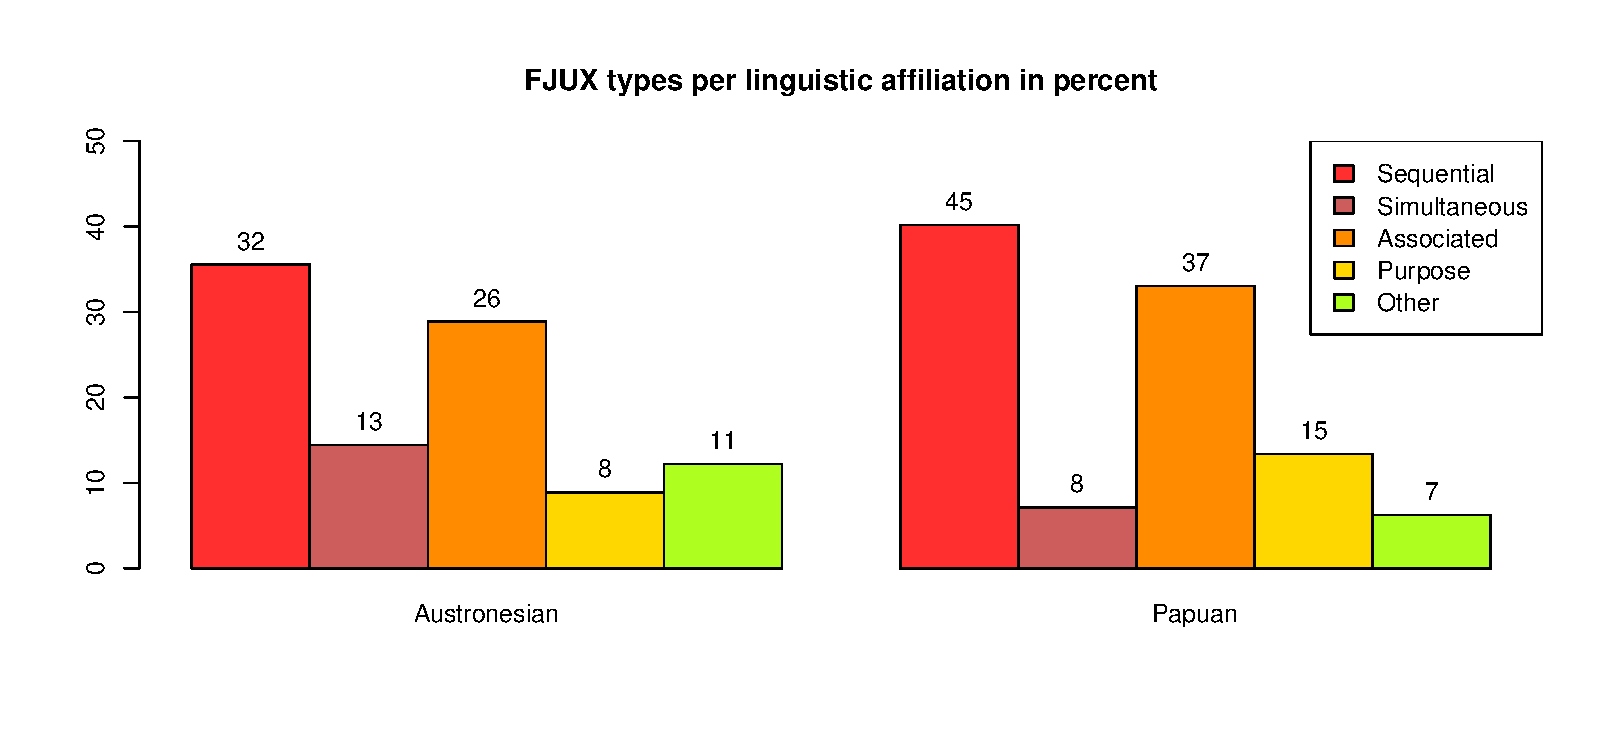
\includegraphics[width=\columnwidth]{figures/FJUX_family.eps}
\caption[FJUX types per linguistic affiliation in percent]{FJUX types per linguistic affiliation in percent. Numbers on top of the bars refer to the number of observations in the sample.}\label{fig:fjux-family}
\end{figure}
\begin{figure}
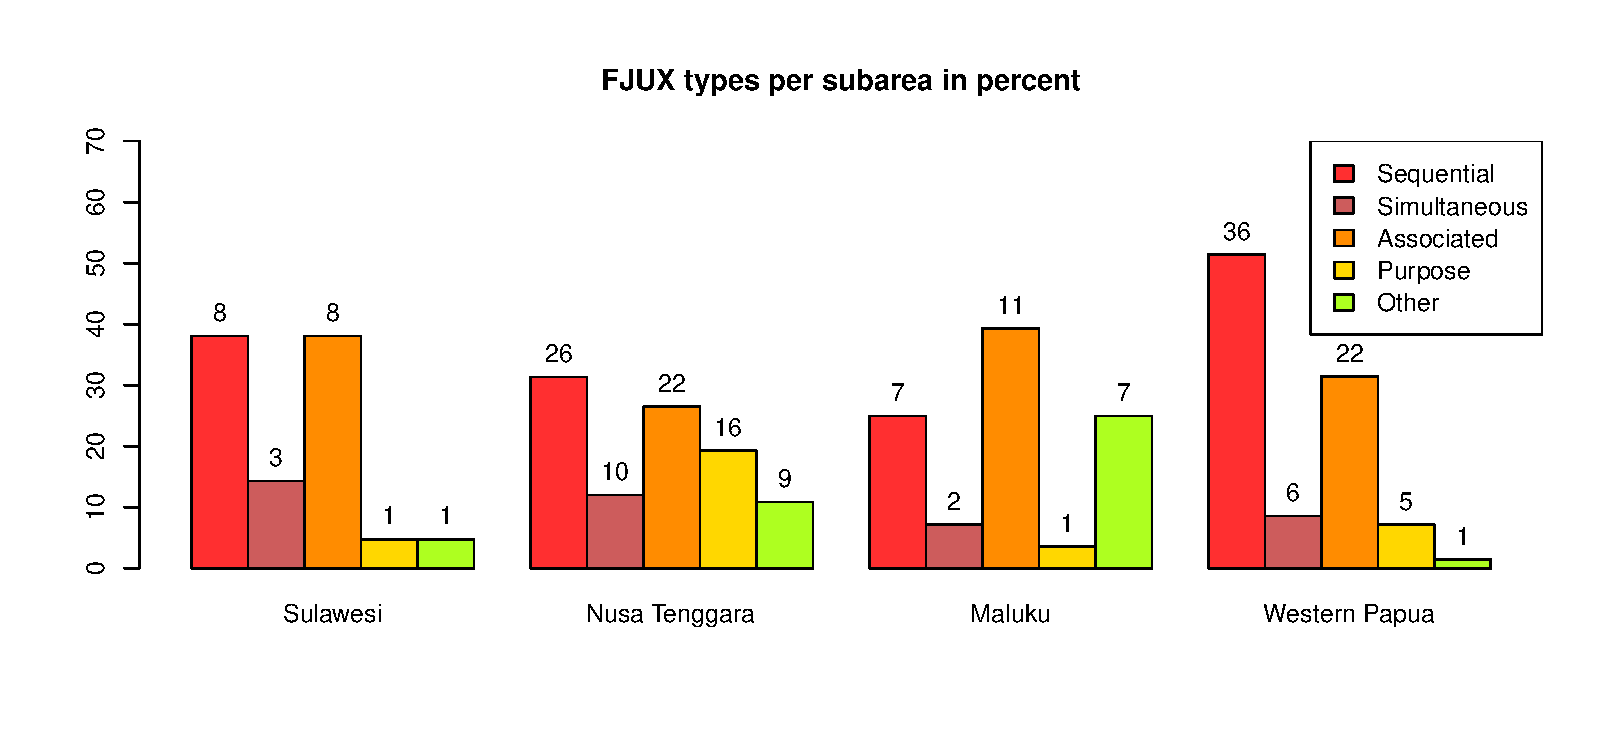
\includegraphics[width=\columnwidth]{figures/FJUX_group.eps}
\caption[FJUX types per subarea in percent]{FJUX types per subarea in percent. Numbers on top of the bars refer to the number of observations in the sample.}\label{fig:fjux-group}
\end{figure}

%The distribution of \textsc{fjux} constructions per language is shown in Table \ref{table:FJUX_language}. 
It is apparent that the numbers are unevenly distributed across the languages. Some languages that are otherwise subject to a high use of different MVC types, such as Abui or Makalero, only show weak traces of \textsc{fjux} use. Other languages with only moderate use of MVC types, such as Mpur or Waima'a, show, for some categories, rather high numbers of occurrence. This appears to reflect different traits, both linguistic and methodological. If we compare the two corpus languages Waima'a and Wooi with over 170 data points each, we observe that the number of attested \textsc{fjux} constructions is rather high in Waima'a, and quite low in Wooi. We can conclude that an increase in the number of data points appears to have an effect on \textsc{fjux} retrieval only in Waima'a, but not in Wooi. This seems to indicate that not all EI languages make regular use of \textsc{fjux} constructions. Another effect that shines through the distribution of \textsc{fjux} cases is the focus of the researcher, and the extent of his or her grammatical description. So, for instance, while most Teiwa examples of sequential MVCs were found in Klamer's chapter on serial verb constructions \citep{klamer2010grammar}, the Mpur examples were (all but one) retrieved from an appended text in \citet{ode2002sketch}. Given that such additional data sources were not available for all languages, chances are high that some languages that appear to make only little use of \textsc{fjux} constructions are in fact undersampled.

%\begin{table}
%\begin{footnotesize}
%\begin{tabular}{lrrrrr}
%  \hline
% & {sequential} & {simultaneous} & {associated} & {purpose} & {other} \\ 
%  \hline
%  Muna &   1 &   1 &   6 &   1 &   1 \\ 
%  Pendau &   0 &   1 &   0 &   0 &   0 \\ 
%  Tajio &   2 &   1 &   1 &   0 &   0 \\ 
%  Tolaki &   2 &   0 &   0 &   0 &   0 \\ 
%  TukangBesi &   3 &   0 &   1 &   0 &   0 \\ %\hline
%  Abui &   1 &   0 &   1 &   2 &   2 \\ 
%  Alorese &   0 &   0 &   0 &   2 &   1 \\ 
%  Bunaq &   0 &   0 &   0 &   3 &   0 \\ 
%  Kaera &   0 &   0 &   0 &   1 &   0 \\ 
%  Kambera &   1 &   1 &   1 &   0 &   0 \\ 
%  Klon &   0 &   0 &   5 &   2 &   0 \\ 
%  Makalero &   1 &   0 &   1 &   0 &   0 \\ 
%  Teiwa &  13 &   2 &   2 &   3 &   1 \\ 
%  Tetun &   3 &   0 &   0 &   0 &   0 \\ 
%  Waima'a &   7 &   7 &  12 &   2 &   5 \\ 
%  Western Pantar &   0 &   0 &   0 &   1 &   0 %\\  \hline
%  Buru &   0 &   0 &   1 &   0 &   3 \\ 
%  Selaru &   1 &   0 &   1 &   0 &   1 \\ 
%  Taba &   2 &   0 &   0 &   0 &   0 \\ 
%  Tidore &   2 &   0 &   8 &   0 &   3 \\ 
%  Tobelo &   2 &   2 &   1 &   1 &   0 \\ \hline
%  Abun &   2 &   0 &   2 &   0 &   0 \\ 
%  Biak &   1 &   0 &   0 &   1 &   0 \\ 
%  Dusner &   0 &   0 &   3 &   2 &   0 \\ 
%  Hatam &   2 &   0 &   0 &   0 &   0 \\ 
%  Inanwatan &   3 &   0 &   4 &   0 &   0 \\ 
%  Maybrat &   4 &   2 &   3 &   0 &   0 \\ 
%  Mor &   4 &   2 &   0 &   0 &   0 \\ 
%  Moskona &   2 &   0 &   4 &   0 &   0 \\ 
%  Mpur &  13 &   2 &   1 &   0 &   1 \\ 
%  Sougb &   0 &   0 &   5 &   2 &   0 \\ 
%  Wooi &   5 &   0 &   0 &   0 &   0 \\ 
%   \hline
%\end{tabular}
%\end{footnotesize}
%\caption[Distribution of \textsc{fjux} types per language]{Distribution of \textsc{fjux} types per language.}
%\label{table:FJUX_language}
%\end{table}

Table \ref{table:FJUX_formal} below presents the morphosyntactic properties of \textsc{fjux} constructions. If \textsc{fjux} constructions are formed at the discourse level, and link independent CLEs together, one might expect a higher amount of variation in formal coding than found with the other constructional families. This appears to be the case, although the prototypical formal setup of MVCs in EI is still visible: most \textsc{fjux} constructions show shared subjects (``S"), both verbs are inflected (``B"), and the verbals stand next to each other without intervening constituents (``C"). Some factorial values are unattested, again matching the prediction. For instance, both participant accumulation (``A") and event-to-argument reanalysis (``E") are hardly or not at all attested. As such referential expressions would point to a close semantic relationship between the CLEs, its absence is predictable. The same goes for headedness patterns denoting a more intricate interplay of the verbal constituents. Both partial head-marking (``1" and ``2") and shared marking (``S") are clearly dispreferred with \textsc{fjux} constructions, as are within-word construals (``W"). The opposite is true for indicators of lower constructional cohesiveness. No referential interaction (``X") occurs frequently, and the contiguity values exceed the ``C" pattern in many cases, i.e., one or more constituents are found to intervene between the verbs.

\begin{table}
\centering
\begin{tabular}{rrrrrrr}
  \lsptoprule
Referentiality & S & SO & D & E & X \\ 
  \hline
  sequential &  52 &   4 &   8 &   1 &  12 \\ 
  simultaneous &  18 &   0 &   0 &   0 &   3 \\ 
  associated &  42 &   3 &   6 &   1 &  11 \\ 
  purpose &  10 &   0 &  11 &   0 &   2 \\ 
  other &  17 &   0 &   0 &   0 &   1 \\ 
   \hline
 \\
  \hline
Headedness & B & 1 & 2 & S & N \\ 
  \hline
  sequential &  44 &   1 &   2 &   0 &   3 \\ 
  simultaneous &  12 &   0 &   0 &   0 &   0 \\ 
  associated &  30 &   2 &   1 &   1 &   5 \\ 
  purpose &   7 &   0 &   0 &   0 &   0 \\ 
  other &   3 &   0 &   0 &   0 &   3 \\ 
   \hline
 \\
  \hline
Contiguity & W & C & 1 & 2 & 3 & 4 \\ 
  \hline
  sequential &   0 &  35 &  31 &  10 &   1 &   0 \\ 
  simultaneous &   0 &  17 &   2 &   2 &   0 &   0 \\ 
  associated &   0 &  33 &  20 &   7 &   2 &   1 \\ 
  purpose &   0 &   8 &  11 &   3 &   1 &   0 \\ 
  other &   2 &  15 &   0 &   1 &   0 &   0 \\ 
   \lspbottomrule
\end{tabular}
\caption[Morphosyntactic properties of \textsc{fjux} constructions]{Morphosyntactic properties of \textsc{fjux} constructions in EI. Table components from top to bottom refer to referentiality (see §\ref{sec:argumentstructure}), headedness (see §\ref{sec:headedness}), and contiguity (see §\ref{sec:contiguity}), respectively.}
\label{table:FJUX_formal}
\end{table}

As in the previous parts of this chapter, the next sections explore the \textsc{fjux} types in some more detail, and provide examples from the different subareas.

\subsection{Sequential}

Sequential MVCs mostly correlate dynamic eventualities, and almost no stative verbs are employed. The constructional meaning is such that both events occur in temporal sequence without, however, an explicit account of how the events are related. Despite the low number of cases, it can be seen from Table \ref{table:sequential} that sequential MVCs can be found in most of the EI languages.

\begin{table}
\begin{tabular}{ll}
\lsptoprule
Feature&Value\tabularnewline
\hline
Template& V1 \textsc{dynamic verb} -- V2 \textsc{dynamic verb}\tabularnewline
No. of attested instances& 77/2146 \tabularnewline
No. of attested languages& 23/32 \tabularnewline
Distribution across areas& \textsc{sul} (4/5), \textsc{nus} (6/11), \textsc{mal} (4/5), \textsc{pap} (9/11) \tabularnewline
Distribution across families& \textsc{pap} (11), \textsc{aus} (12) \tabularnewline
\lspbottomrule
\end{tabular}
\caption[Template and basic distribution of sequential MVCs]{Template and basic distribution of sequential MVCs in the EI sample.}
\label{table:sequential}
\end{table}

The following examples demonstrate that sequential MVCs can adapt to many different contexts and communicative situations. Example (\ref{Tukang_49}) from Tukang Besi depicts a classical combination of two dynamnic events. The second event begins just when the first event happens to end. There is no specific relation between the gossiping and the continuing, such as causal or consecutive relations. Notice also that there is no referential identity in the narrow sense. 

\ea \label{Tukang_49}
\langinfo{Tukang Besi}{Austronesian, WMP}{\citealt[503]{donohue1999}}\\
\gll po'oli ko-tula-tula ku-torusu-mo ku(a) koranga \\
finish 1\textsc{pa}.\textsc{rls}-\textsc{rdp}-tale 1\textsc{sg}-continue-\textsc{prfv} \textsc{all} garden \\
\glft `After we had gossiped, I continued on to the garden.'\\ 
\z

Another group of sequential MVCs denotes action sequences in which the actor remains constant. The next two examples in (\ref{Tetun_13}) and (\ref{Tidore_87}) from Tetun and Tidore, respectively, illustrate such use. In example (\ref{Tetun_13}), we can see a sequence of seven verbs. \citet{vanklinken1999grammar} tentatively placed clausal boundaries between \textit{manas} and \textit{hodi}, and between \textit{mai} and \textit{sia}, but from the lack of prosodic and syntactic boundary clues one could also argue for a free juxtaposition of several smaller MVCs that are aligned here because they all happen in what is perceived as one discourse sequence. It is remarkable that the verbal building blocks fall into MVC types that are immediately recognisable: \textit{bá te'in} form a motion-to-action construction, \textit{nono wé manas} constitute a resultative construction, and \textit{hodi mai} is a transport complex. Two linkings, however, do not fit into any of the constructions types discussed previously in this chapter. First, there is no construction that would comprise a combination of cooking and heating. As both verbs are at least in this context quasi synonymous they can be regarded as a lexicalised combination, created by stylistic conventions rather than by communicative needs (recall the synonymous verbs from §\ref{sec:other}). And second, bringing and drinking is special due to the change in referential expression. It is not the actor bringing the hot water that drinks it afterwards. Rather the construction looks like a purpose construction (I will come back to this type in section §\ref{sec:purpose}). 

\ea \label{Tetun_13}
\langinfo{Tetun Fehan}{Austronesian}{\citealt[253]{vanklinken1999grammar}}\\
\gll bá te'in nono wé manas hodi mai sia r-emu \\
go cook heat(.liquid) water hot bring come 3\textsc{pl} 3\textsc{pl}-drink \\
\glft `[Then] (I) went and boiled water and brought (it and) they drank [, and they ate.]'\\ 
\z

The verb string in example (\ref{Tidore_87}) denotes a procedure involving three actions (all having a different object). Each step leads to the next one until the body of the participant is smeared with fish blood. Such procedures are often associated with manual action, and there are several cases of \textsc{fjux} attested for such procedurals in the dataset.

\ea \label{Tidore_87}
\langinfo{Tidore}{Papuan, NH}{\citealt[368]{vanstaden2000tidore}}\\
\gll Ah, ona yau wako isa=ge, ona suka nyao ngge oro ena ma-au se-baca una i-rehe ena=ge \\
ah 3\textsc{pl} to.fish return landwards=there 3\textsc{pl} break fish 3\textsc{nhum}.there take 3\textsc{nhum} 3\textsc{nhum}.\textsc{pos}-blood \textsc{caus}-\textsc{nm}.rub 3\textsc{sg}.\textsc{m} 3\textsc{sg}.\textsc{m}.\textsc{pos}-body 3\textsc{nhum}=there \\
\glft ‘So when they returned from fishing they cut up a fish and took its blood and rubbed his body.’\\ 
\z

The last example is from Abun. As in example (\ref{Tetun_13}) from Tetun, it appears to juxtapose two MVCs, a motion-to-action construction and a transport complex, together. Unfortunately, Berry and Berry's grammar of Abun does not provide appended texts, and it cannot be ascertained at this point whether \textsc{fjux} construals are a regular means of composing MVCs in Abun. What is remarkable with such conjoined MVCs is that they form templates just as the ones Pawley describes for Kalam.

\ea \label{Abun_4}
\langinfo{Abun}{Papuan, isolate}{\citealt[52]{berry1999}}\\
\gll ye-suk-mise ma nai gwat an mu ket \\
\textsc{pers}-\textsc{nm}-evil come capture carry 3\textsc{sg} go west \\
\glft `The police came and caught him and took him westward.'\\ 
\z

\subsection{Simultaneous} \label{sec:simultaneous}

Simultaneous \textsc{MVC}s are vey infrequent in the EI sample, with only 21 examples from ten languages. Table \ref{table:simultaneous} provides the numbers. Most simultaneous instances denote a motion event, together with another action that is carried out by the moving participant. There are no stative verbs found in simultaneous MVCs.

\begin{table}
\begin{tabular}{ll}
\lsptoprule
Feature&Value\tabularnewline
\hline
Template& V1 \textsc{dynamic verb} -- V2 \textsc{dynamic verb}\tabularnewline
No. of attested instances& 21/2146 \tabularnewline
No. of attested languages& 10/32 \tabularnewline
Distribution across areas& \textsc{sul} (3/5), \textsc{nus} (3/11), \textsc{mal} (1/5), \textsc{pap} (3/11) \tabularnewline
Distribution across families& \textsc{pap} (4), \textsc{aus} (6) \tabularnewline
\lspbottomrule
\end{tabular}
\caption[Template and basic distribution of simultaneous MVCs]{Template and basic distribution of simultaneous MVCs in the EI sample.}
\label{table:simultaneous}
\end{table}

Here are two examples of simultaneous MVCs. Example (\ref{Pendau_4}) from Pendau illustrates the combination of a manner of motion verb with a state change verb. As the flying proceeds, the shapes of the referents become smaller against the sky. Note that the aspectual clitic \textit{=mo} attaches to the last verb in the series, and the scope of the completive is over the whole simultaneous construction. Similar scope behaviour can also be observed in other EI languages. Take the example from Teiwa in (\ref{Teiwa_37}) in which a progressive marker is placed in construction-final position. Here, as well, it seems that the scope of \textit{pati} is over the whole construction. 

\ea \label{Pendau_4}
\langinfo{Pendau}{Austronesian, WMP}{\citealt[335]{Quick2007}}\\
\glll bai uo nolumeap nkaasimo, jimo no'umene' \\
bai 'uo N-po-[um]-leap no-kaasi=mo jimo no-'u-mene' \\
like yonder \textsc{rls}-\textsc{sf}-\textsc{tel}-fly \textsc{st}.\textsc{rls}-shrink=\textsc{compl} 3\textsc{pl}.\textsc{abs} \textsc{ug}.\textsc{rls}-\textsc{sf}-go.up \\
\glft `So as they flew up they shrunk (in apparent size), and they went up.'\\ 
\z

\ea \label{Teiwa_37}
\langinfo{Teiwa}{Papuan, TAP}{\citealt[312]{klamer2010grammar}}\\
\gll bai qavif non saxa' rau, kamau, a-tan pin-an soxai pati \\
pig goat \textsc{pl} chicken civet.cat cat \textsc{top} 3\textsc{sg}-stand hold-\textsc{rls} dance \textsc{prog} \\
\glft `[the] pigs, goats, chicken, civet cats, cats, who were holding hands while dancing.'\\ 
\z

Teiwa, as well as other EI languages, also has formal means to conjoin two eventualities. In Teiwa, there is a junctor \textit{si} that correlates two clauses the eventualities of which happen at the same time. While cases like example (\ref{Teiwa_37}) still appear to form a tight construal, and share their subject referents, simultaneous structures marked with \textit{si} appear to combine larger units. Consider the following example. There is a switch in reference between both events. The subject of V$_1$ becomes the goal of the climbing. Such simultaneous markers are also attested in other EI languages. If they constitute clause linking devices, then the simultaneous MVCs illustrated above still produce more compressed biclausal structures, or may even turn out to form a single clause, as the operator behaviour seems to suggest in some cases.

\ea \label{}
\langinfo{Teiwa}{Papuan, TAP}{\citealt[257]{klamer2010grammar}}\\
\gll ti'-in, iqa'an ga'an u a un tii'-in si ilan mir \\
sleep-\textsc{rls} dark 3\textsc{sg} \textsc{dist} 3\textsc{sg} \textsc{cont} sleep-\textsc{rls} \textsc{sim} grow.up ascend \\
\glft `Sleeping...that night he was sleeping while [something] came up [to him].'\\ 
\z

\subsection{Associated}

In associated MVCs the temporal relation between the verbs seems less prominent than in the sequential or simultaneous construction. What is foregrounded instead is a general notion of both eventualities being associated with each other. This association is in most cases reminiscent of semantic relations otherwise found in clause subordination, such as conditional, adversative, or conclusive semantics. In some cases, but not in all, a junctor may be placed between the verbs without any apparent change in meaning. With only 20 attested cases, associated MVCs lack sufficient data for a more detailed analysis, and I doubt that, with more data at hand, this will turn out to be a coherent construction throughout EI. Table \ref{table:associated} illustrates the basic numbers.

\begin{table}
\begin{tabular}{ll}
\lsptoprule
Feature&Value\tabularnewline
\hline
Template& V1 \textsc{verb} -- V2 \textsc{verb}\tabularnewline
No. of attested instances& 63/2146 \tabularnewline
No. of attested languages& 20/32 \tabularnewline
Distribution across areas& \textsc{sul} (3/5), \textsc{nus} (6/11), \textsc{mal} (4/5), \textsc{pap} (7/11) \tabularnewline
Distribution across families& \textsc{pap} (11), \textsc{aus} (12) \tabularnewline
\lspbottomrule
\end{tabular}
\caption[Template and basic distribution of associated MVCs]{Template and basic distribution of associated MVCs in the EI sample.}
\label{table:associated}
\end{table}

Consider the following examples. In example (\ref{Muna_2}) from Muna we can see a MVC that looks just like a conditional clause. \citet{vandenberg1989} remarks that one may add the conditional marker \textit{ane} here without making any change to the meaning. While the singing appears to refer to an individuable spatiotemporal event, the voice being beautiful can be regarded as an individual-level predicate that holds true not only at the time of the singing, but constitutes a permanent property of the participant. Therefore, such construals seem to be different from simultaneous MVCs where two actions are correlated and performed by one single actor. The next example in (\ref{Teiwa_74}) is from Teiwa and illustrates adversative semantics. This example  demonstrates a case in which no referential interaction takes place (no argument sharing, ``X" pattern). Note also that the second clause is negated with \textit{maan}, while the first clause is not. This is a strong clue that we are dealing here with two independent clauses.

\ea \label{Muna_2}
\langinfo{Muna}{Austronesian, WMP}{\citealt[235]{vandenberg1989}}\\
\gll nao-kesa sepaliha dua suara-no (ane) nae-lagu \\
3\textsc{sg}.\textsc{irr}-beautiful very also voice-his (if) 3\textsc{sg}.\textsc{irr}-sing \\
\glft `His voice will also be very beautiful when he sings.'\\ 
\z

\ea \label{Teiwa_74}
\langinfo{Teiwa}{Papuan, TAP}{\citealt[355]{klamer2010grammar}}\\
\gll suk-an maan kri u pak-an pak-an suk-an maan \\
exit.come.down-\textsc{rls} \textsc{neg} Mr \textsc{dist} call-\textsc{rls} call-\textsc{rls} exit.come.down-\textsc{rls} \textsc{neg} \\
\glft `They didn't come out, that grandfather called and called [but] no-one came out...'\\ 
\z

The next example from Tobelo shows two conjoined statives. Just like \textit{kesa} `be beautiful' in example (\ref{Muna_2}) from Muna, \textit{bole} `be tired' and \textit{timono} `old' are, in my view, understood as individual-level predicates, denoting permanent properties of the participant. Although one may claim that both states hold true at event time, they hardly constitute simultaneous events in the sense discussed in §\ref{sec:simultaneous}. The last example in (\ref{Sougb_36}) from Sougb shows two action verbs, \textit{(o)uhw} `trade' and \textit{ebe-piara} `do-look.after', that occur in temporal sequence, but differ from typical sequential constructions in that the second verb projects an event that extends over years instead of denoting a concrete (manual) action within a limited time span. A second property that is not found in prototypical sequential MVCs is the function switch from first person object to first person subject. The first person participant here acts like a pivotal argument, leading to what seems to be an overlap of two clauses. Indeed, such construals bear a resemblance to those constructions in West African languages that \citet{ameka2005multiverb} described as overlapping constructions.

\ea \label{}
\langinfo{Tobelo}{Papuan, NH}{\citealt[68]{holton2003tobelo}}\\
\gll i-hi-bole-oka i-hi-timono-oka ho to-oiki-oka-ua \\
3-1-tired-\textsc{prfv} 3-1-old-\textsc{prfv} thus 1-go-\textsc{prfv}-\textsc{neg} \\
\glft `I was old and tired, so I didn't want to go again.'\\ 
\z

\ea \label{Sougb_36}
\langinfo{Sougb}{Papuan, EBH}{\citealt[269]{reesink2002grammar}}\\
\gll dan d-ouma, gida hom, ka lan la-(o)uhw dou dan d-ebe-piara \\
I 1\textsc{sg}-buy female one then they.\textsc{du} 2\textsc{du}-trade to I 1\textsc{sg}-do-look.after \\
\glft `I would buy one girl and they'd trade her to me and I would look after her.'\\ 
\z

In the next section, I turn to purpose MVCs that also appear to be construed much like overlapping constructions in West African languages.

\subsection{Purpose} \label{sec:purpose}

Purpose MVCs combine two action predicates, of which the second one denotes the outcome or purpose of the first action. The actor of the first predicate is typically not maintained in the second predicate. The most frequent verb in V$_1$ is a verb of giving or putting. An actor transfers some object to another (group of) participant(s) in order for them to perform some other action. Given that the number of attested constructions is quite low in the dataset, the number of languages with attested cases is rather high (n=13). We can see from Table \ref{table:purpose} that the use of the purpose construction is predominantly found in Nusa Tenggara languages.

\begin{table}
\begin{tabular}{ll}
\lsptoprule
Feature&Value\tabularnewline
\hline
Template& V1 \textsc{dynamic verb} -- V2 \textsc{dynamic verb}\tabularnewline
No. of attested instances& 23/2146 \tabularnewline
No. of attested languages& 13/32 \tabularnewline
Distribution across areas& \textsc{sul} (1/5), \textsc{nus} (8/11), \textsc{mal} (1/5), \textsc{pap} (3/11) \tabularnewline
Distribution across families& \textsc{pap} (8), \textsc{aus} (5) \tabularnewline
\lspbottomrule
\end{tabular}
\caption[Template and basic distribution of purpose MVCs]{Template and basic distribution of purpose MVCs in the EI sample.}
\label{table:purpose}
\end{table}

The following examples present typical cases from different subareas. In example (\ref{Bunaq_4}) from Bunaq, a \textsc{give} verb is combined with a verb of food consumption. This is indeed the most widespread combination (mostly with \textsc{eat} verbs). Schapper analysed this construction type as causative SVCs, ``expressing purposive causation in transfer events" \citep[446]{schapper2009bunaq}. Arguably, there is indeed some sense of causation involved between the transfer and the consequent action in that it is the transfer that \emph{enables} the second action to be carried out. Such construals of causation differ, however, from direct causation, as construed by cause-result, causative or resultative constructions in the EI area. While in those constructions we may say that the initial causing event directly triggers the resultant event (for instance, because some force is applied to a patient participant), in purpose MVCs the second action may or may not be carried out. It seems that the purposive reading leaves the actual performance of the second event unexpressed. So, for instance, in example (\ref{Bunaq_4}) we do in fact not really know whether the drinking event will take place or not. It is only that the transfer enables the third person participant to carry out the drinking. 

\ea \label{Bunaq_4}
\langinfo{Bunaq}{Papuan, TAP}{\citealt[446]{schapper2009bunaq}}\\
\gll neto baqi g-ege il a \\
1\textsc{sg} \textsc{nprx}.\textsc{an} 3\textsc{an}-give water drink \\
\glft ‘I gave him water to drink.’\\ 
\z

This non-realis interpretation of the second action becomes visible when negation is applied to the construction, as we can see in example (\ref{Bunaq_4b}) below. While it is fine for the negator to have scope over the whole construction, it may not be place before the second verb. This suggests that the drinking may not be negated because it has in fact not yet taken place. 

\ea \label{Bunaq_4b}
\langinfo{Bunaq}{Papuan, TAP}{\citealt[446]{schapper2009bunaq}}\\
\ea
\gll neto baqi g-ege il a niq \\
1\textsc{sg} \textsc{nprx}.\textsc{an} 3\textsc{an}-give water drink \textsc{neg} \\
\glft ‘I did not give him water to drink.’ \\ 
\ex
\gll *neto baqi g-ege niq il a \\ 
1\textsc{sg} \textsc{nprx}.\textsc{an} 3\textsc{an}-give \textsc{neg} water drink \\
\z
\z

Example (\ref{Alorese_17}) from Alorese suggests a similar MVC. The transfer of pictures is intended to let another participant look at them. Notice that the first person referent is expressed here twice by a free pronoun. Expressing one participant twice would be clearly dispreferred in most MVC types with a closer packing of LLEs, and this can be interpreted as another clue for rather loose bonds between the two predicates here. Example (\ref{Tobelo_16}) from Tobelo shows yet another combination of verbs. In this example, the actors stay the same across both predicates, but the translation still indicates a purposive interpretation. Finally, the Dusner example in (\ref{Dusner_4}) illustrates another purposive combination with an \textsc{eat} verb in final position. Here as well, the actor is the same in both predicates.

\ea \label{Alorese_17}
\langinfo{Alorese}{Austronesian, CMP}{\citealt[72]{klamer2011alorese}}\\
\gll mi neng go foto go seru \\
2\textsc{pl} give 1\textsc{sg} photograph 1\textsc{sg} see \\
\glft `You show me (some) pictures.' (Lit. You give me pictures I see) \\ 
\z

\ea \label{Tobelo_16}
\langinfo{Tobelo}{Papuan, NH}{\citealt[61]{holton2003tobelo}}\\
\gll yo-karajanga o-lapangan yo-diai \\
3\textsc{pl}-work \textsc{nm}-field 3\textsc{pl}-make \\
\glft `We [sic] worked to make an airfield.' \\ 
\z

\ea \label{Dusner_4}
\langinfo{Dusner}{Austronesian, SHWNG}{\citealt[19]{dalrymple2012}}\\
\glll yave o verano yan \\
ya-ve o Ø-ve-ran=o y-an \\
1\textsc{sg}-say \textsc{exclam} 1\textsc{sg}-\textsc{vblz}-sago=\textsc{fill} 1\textsc{sg}-eat \\
\glft `I said: Oh, I can make papeda (sago porridge) to eat.'\\ 
\z

\subsection{Other}

The final group of examples from free juxtaposition constructions comprise two smallish sets of MVCs. First, there are two cases of delimitative MVCs (do x \textit{until} y happens), one from Mpur and another one from Muna. I have already discussed this construction at the beginning of §\ref{sec:fjux}, and have nothing to add here. Second, there is a small set of verb collocations that appear to be, to a certain extent, lexicalised, and thus may occur together in fixed chunks. I will not have much to say about these groups as there is so little data available. Neither is it possible to examine in detail whether these collocations really do behave as fixed expressions, so that some of these cases might instead simply turn out to be `the odd ones out'.

As lexicalised verb strings may even exhibit word-like properties, their placement within free juxtaposition constructions is clearly only preliminary. Although lexicalised construals would arguably be construed rather tightly, I assume that they might have originated in more loose collocations. Table \ref{table:other_fjux} illustrates the distribution of this heterogeneous group. Lexicalised MVCs of different kinds seem to be more in use in Nusa Tenggara and Maluku. 

\begin{table}
\begin{tabular}{ll}
\lsptoprule
Feature&Value\tabularnewline
\hline
Template& V1 \textsc{dynamic verb} -- V2 \textsc{dynamic verb}\tabularnewline
No. of attested instances& 18/2146 \tabularnewline
No. of attested languages& 9/32 \tabularnewline
Distribution across areas& \textsc{sul} (1/5), \textsc{nus} (4/11), \textsc{mal} (3/5), \textsc{pap} (1/11) \tabularnewline
Distribution across families& \textsc{pap} (4), \textsc{aus} (5) \tabularnewline
\lspbottomrule
\end{tabular}
\caption[Template and basic distribution of other \textsc{fjux} MVCs]{Template and basic distribution of other \textsc{fjux} MVCs in the EI sample.}
\label{table:other_fjux}
\end{table}

We have already seen one type of lexicalised MVC in the component-relating family, namely synonymous MVCs (see §\ref{sec:other}). I argued there that synonymous \textsc{crel}s bear a resemblance to other component-relating constructions as the verbs obviously share at least some part of their semantic structure. Some authors have extended the notion of synonymous SVCs to cases in which two verbs with related semantics (from the ``same semantic field") are combined. Example (\ref{Abui_34}) from Abui shows two such MVCs. The first pair of verbs with somewhat ``related semantics" is \textit{t} `lie' and \textit{wel} `pour', at least understood in a non-literal sense as pertaining to daily processes in the upbringing of a child. Another pair is claimed to consist of \textit{fok-d} `big-hold' and \textit{fin-r} `eldest-reach', both relating to growing up in a wider sense. Kratochvíl placed these constructions with the group of synonymous SVCs, and remarked that ``[t]hese parallel expressions seem to be lexicalized or at least highly conventionalized" (2007: 357). The difference to synonymous MVCs \textit{sensu stricto}, however, is that the verbs only share very unspecific meaning components, if any at all.

\ea \label{Abui_34}
\langinfo{Abui}{Papuan, TAP}{\citealt[357]{kratochvil2007grammar}}\\
\gll na a-t a-wel-i ba he-fokda he-fin-r-i \\
1\textsc{sg} 2\textsc{sg}.\textsc{pat}-lie 2\textsc{sg}.\textsc{pat}-pour-\textsc{prfv} \textsc{lnk} 3\textsc{loc}-grow.up 3\textsc{loc}-eldest-reach-\textsc{prfv} \\
\glft ‘I took care of you till you grew up.’ (lit: ‘I fed and washed you until you grew up and
became adult’)\\
\z

Another example of lexicalised MVCs is the following combination of a \textsc{see} verb and a \textsc{find} verb from Waima'a. The examples are from two pear story narrations, each narrated by a different speaker. Both speakers use exactly the same construction at the point where the boy is handed back his hat. Note that both verbs are placed next to each other, and all expressed arguments are found either before or after the verb complex.

\ea \label{}
\langinfo{Waima'a}{Austronesian, CMP}{pear\_Bendita 039}\\
\gll ne: buni hita hile lo ne zapeu nini \\
\textsc{foc} see find again \textsc{asp} 3\textsc{sg} hat \textsc{poss} \\
\glft `...and found his hat.'\\ 
\z

\ea \label{}
\langinfo{Waima'a}{Austronesian, CMP}{pear\_Santina 171}\\
\glll ne bun hita sapeo anse \\
ne buni hita sabeo ana-see \\
\glc 3\textsc{sg} see find hat \textsc{clf}-one \\
\glft `He finds a hat...' \\ 
\z

In the light of what I have discussed in this chapter and the previous one, free juxtaposition constructions are ephemeral constructions that can be perceived as \textit{ad hoc} formations on the discourse-level rather than as fixed constructions with rigid constructional blueprints, such as, say, motion complex MVCs with their invariant order ot motion verb classes. Rather, any combination of verbs seems licit as long as more general rules of semantic clause linking are adhered to. In this view, lexicalised, or at least condensed verb structures without a host class slot, such as we have seen in the Waima'a examples above, do not seem to fit into the \textsc{fjux} category, and may instead constitute a category of their own.

\section{Summary}

This chapter explored the dataset with regard to constructional types and their distribution across Eastern Indonesia. By combining the morphosyntactic findings from Chapter \ref{ch:gram} with the semantic theory of MVC formation on different conceptual levels developed in Chapter \ref{ch:sem}, I proposed four families of MVCs used throughout the region. Each constructional family is based upon one underlying technique of MVC formation. While both component-relating constructions and modifying constructions constitute single-stage MVCs with only one individuable event stage based on a single (combined) event argument, stage-relating constructions and free juxtaposition constructions correlate two event expressions by forming a two-stage event schema. The event argument of each verb is in these types preserved, and each may in principle become the target of a grammatical operator. However, as we have seen, stage-relating constructions appear to be the result of a certain extent of grammaticalisation, at least in some of the EI languages, preventing the staged constituents to act like fully independent constituents. 

In §\ref{sec:criteria_mvcs} I presented a set of criteria that, when applied together, reveals differences between the four constructional families. The criteria were taken from four fields: argument structure, operator behaviour, constituency, and semantics. Four criteria set off \textsc{fjux} constructions from the other three types. Obligatory argument interaction, identical TAM/person index values, and asymmetrical headedness are not found in \textsc{fjux}, but in all other constructional families. Conjunction insertion, on the other hand, is only found with \textsc{fjux} constructions. Five additional criteria distinguish the single-stage construction types \textsc{crel} and \textsc{mod} from the two-stage \textsc{srel} and \textsc{fjux} types. Both event-to-argument reanalysis and grammaticalisation of features in V$_2$ are associated with the former, but not with the latter. Partial temporal modification and sequential reading, on the other hand, are only indicative of the two-stage types, and not of the single-stage ones \textsc{crel} and \textsc{mod}. Partial negation appears to be licit in \textsc{mod} and \textsc{fjux}, but not in \textsc{crel} and \textsc{srel}. Finally, some criteria are unique to certain types. Obligatory constituent order is found with all types except \textsc{mod}. MVC embedding seems possible with all types but \textsc{crel}. And the notion of temporal immediacy holding between the verbs' event schemas is a feature of \textsc{srel} constructions, but is not present in or not necessarily inferable from the other three types.

The distribution of MVCs is surprisingly even across linguistic affiliation and geographical subareas. Linguistic affiliation is, in all likelihood, not a major factor in predicting the occurrence of MVC types. The four subareas, Sulawesi, Nusa Tenggara, Maluku, and Western Papua, showed moderate differences in the use of MVC types. Modifying constructions were found to be most frequent in the former three subareas, while in Western Papua the use of component-relating constructions and stage-relating constructions was slightly more frequent than \textsc{mod} constructions. Biclausal free juxtaposition constructions were in all four subareas only attested in small numbers. 

In the final chapter, I will attempt to review the findings from this book and draw some preliminary conclusions that arise from the data. The focus will be on interpreting the patterns of MVC usage further, and hinting at some observations that could not be included into the discussion of the previous chapters.